% Options for packages loaded elsewhere
\PassOptionsToPackage{unicode}{hyperref}
\PassOptionsToPackage{hyphens}{url}
\documentclass[
]{article}
\usepackage{xcolor}
\usepackage[margin=1in]{geometry}
\usepackage{amsmath,amssymb}
\setcounter{secnumdepth}{5}
\usepackage{iftex}
\ifPDFTeX
  \usepackage[T1]{fontenc}
  \usepackage[utf8]{inputenc}
  \usepackage{textcomp} % provide euro and other symbols
\else % if luatex or xetex
  \usepackage{unicode-math} % this also loads fontspec
  \defaultfontfeatures{Scale=MatchLowercase}
  \defaultfontfeatures[\rmfamily]{Ligatures=TeX,Scale=1}
\fi
\usepackage{lmodern}
\ifPDFTeX\else
  % xetex/luatex font selection
\fi
% Use upquote if available, for straight quotes in verbatim environments
\IfFileExists{upquote.sty}{\usepackage{upquote}}{}
\IfFileExists{microtype.sty}{% use microtype if available
  \usepackage[]{microtype}
  \UseMicrotypeSet[protrusion]{basicmath} % disable protrusion for tt fonts
}{}
\makeatletter
\@ifundefined{KOMAClassName}{% if non-KOMA class
  \IfFileExists{parskip.sty}{%
    \usepackage{parskip}
  }{% else
    \setlength{\parindent}{0pt}
    \setlength{\parskip}{6pt plus 2pt minus 1pt}}
}{% if KOMA class
  \KOMAoptions{parskip=half}}
\makeatother
\usepackage{color}
\usepackage{fancyvrb}
\newcommand{\VerbBar}{|}
\newcommand{\VERB}{\Verb[commandchars=\\\{\}]}
\DefineVerbatimEnvironment{Highlighting}{Verbatim}{commandchars=\\\{\}}
% Add ',fontsize=\small' for more characters per line
\usepackage{framed}
\definecolor{shadecolor}{RGB}{248,248,248}
\newenvironment{Shaded}{\begin{snugshade}}{\end{snugshade}}
\newcommand{\AlertTok}[1]{\textcolor[rgb]{0.94,0.16,0.16}{#1}}
\newcommand{\AnnotationTok}[1]{\textcolor[rgb]{0.56,0.35,0.01}{\textbf{\textit{#1}}}}
\newcommand{\AttributeTok}[1]{\textcolor[rgb]{0.13,0.29,0.53}{#1}}
\newcommand{\BaseNTok}[1]{\textcolor[rgb]{0.00,0.00,0.81}{#1}}
\newcommand{\BuiltInTok}[1]{#1}
\newcommand{\CharTok}[1]{\textcolor[rgb]{0.31,0.60,0.02}{#1}}
\newcommand{\CommentTok}[1]{\textcolor[rgb]{0.56,0.35,0.01}{\textit{#1}}}
\newcommand{\CommentVarTok}[1]{\textcolor[rgb]{0.56,0.35,0.01}{\textbf{\textit{#1}}}}
\newcommand{\ConstantTok}[1]{\textcolor[rgb]{0.56,0.35,0.01}{#1}}
\newcommand{\ControlFlowTok}[1]{\textcolor[rgb]{0.13,0.29,0.53}{\textbf{#1}}}
\newcommand{\DataTypeTok}[1]{\textcolor[rgb]{0.13,0.29,0.53}{#1}}
\newcommand{\DecValTok}[1]{\textcolor[rgb]{0.00,0.00,0.81}{#1}}
\newcommand{\DocumentationTok}[1]{\textcolor[rgb]{0.56,0.35,0.01}{\textbf{\textit{#1}}}}
\newcommand{\ErrorTok}[1]{\textcolor[rgb]{0.64,0.00,0.00}{\textbf{#1}}}
\newcommand{\ExtensionTok}[1]{#1}
\newcommand{\FloatTok}[1]{\textcolor[rgb]{0.00,0.00,0.81}{#1}}
\newcommand{\FunctionTok}[1]{\textcolor[rgb]{0.13,0.29,0.53}{\textbf{#1}}}
\newcommand{\ImportTok}[1]{#1}
\newcommand{\InformationTok}[1]{\textcolor[rgb]{0.56,0.35,0.01}{\textbf{\textit{#1}}}}
\newcommand{\KeywordTok}[1]{\textcolor[rgb]{0.13,0.29,0.53}{\textbf{#1}}}
\newcommand{\NormalTok}[1]{#1}
\newcommand{\OperatorTok}[1]{\textcolor[rgb]{0.81,0.36,0.00}{\textbf{#1}}}
\newcommand{\OtherTok}[1]{\textcolor[rgb]{0.56,0.35,0.01}{#1}}
\newcommand{\PreprocessorTok}[1]{\textcolor[rgb]{0.56,0.35,0.01}{\textit{#1}}}
\newcommand{\RegionMarkerTok}[1]{#1}
\newcommand{\SpecialCharTok}[1]{\textcolor[rgb]{0.81,0.36,0.00}{\textbf{#1}}}
\newcommand{\SpecialStringTok}[1]{\textcolor[rgb]{0.31,0.60,0.02}{#1}}
\newcommand{\StringTok}[1]{\textcolor[rgb]{0.31,0.60,0.02}{#1}}
\newcommand{\VariableTok}[1]{\textcolor[rgb]{0.00,0.00,0.00}{#1}}
\newcommand{\VerbatimStringTok}[1]{\textcolor[rgb]{0.31,0.60,0.02}{#1}}
\newcommand{\WarningTok}[1]{\textcolor[rgb]{0.56,0.35,0.01}{\textbf{\textit{#1}}}}
\usepackage{graphicx}
\makeatletter
\newsavebox\pandoc@box
\newcommand*\pandocbounded[1]{% scales image to fit in text height/width
  \sbox\pandoc@box{#1}%
  \Gscale@div\@tempa{\textheight}{\dimexpr\ht\pandoc@box+\dp\pandoc@box\relax}%
  \Gscale@div\@tempb{\linewidth}{\wd\pandoc@box}%
  \ifdim\@tempb\p@<\@tempa\p@\let\@tempa\@tempb\fi% select the smaller of both
  \ifdim\@tempa\p@<\p@\scalebox{\@tempa}{\usebox\pandoc@box}%
  \else\usebox{\pandoc@box}%
  \fi%
}
% Set default figure placement to htbp
\def\fps@figure{htbp}
\makeatother
\setlength{\emergencystretch}{3em} % prevent overfull lines
\providecommand{\tightlist}{%
  \setlength{\itemsep}{0pt}\setlength{\parskip}{0pt}}
\usepackage{fvextra}
\DefineVerbatimEnvironment{Highlighting}{Verbatim}{breaklines,commandchars=\\\{\}}
\RecustomVerbatimEnvironment{verbatim}{Verbatim}{breaklines}

\usepackage{booktabs}
\usepackage{caption}
\usepackage{longtable}
\usepackage{colortbl}
\usepackage{array}
\usepackage{anyfontsize}
\usepackage{multirow}
\usepackage{bookmark}
\IfFileExists{xurl.sty}{\usepackage{xurl}}{} % add URL line breaks if available
\urlstyle{same}
\hypersetup{
  pdftitle={Variance Estimation from SAS Poulpe to R Gustave},
  pdfauthor={Thomas Delclite},
  hidelinks,
  pdfcreator={LaTeX via pandoc}}

\title{Variance Estimation from SAS Poulpe to R Gustave}
\author{Thomas Delclite}
\date{29/05/2026}

\begin{document}
\maketitle

{
\setcounter{tocdepth}{2}
\tableofcontents
}
\section{Introduction}\label{introduction}

This vignette documents the migration of variance estimation workflows
from the SAS \texttt{Poulpe} macro to R, using the \texttt{gustave}
package developed by INSEE. This vignette is intended for survey
methodologists migrating from the SAS Poulpe macro to R, or for
methodologists who need to implement analytical variance estimation for
complex surveys.

The core outcome is a set of \textbf{variance estimation wrappers}:
self-contained R functions that encapsulate the full sampling
methodology (stratification, non-response correction, calibration,
multi-stage sampling) and can be distributed to thematic units. Once a
wrapper has been prepared by the methodologist, analysts can compute
precision measures on their own datasets with a single function call ---
without needing to understand the underlying formulas. Wrappers can also
be called from Python through \texttt{rpy2}, allowing seamless
integration into existing analytical pipelines.

We have validated the R implementation against \texttt{Poulpe} reference
values across five progressively complex cases, from simple stratified
sampling to two-stage designs with individual-level estimation. The
results match, confirming that \texttt{gustave} fully replaces
\texttt{Poulpe} for the survey designs used at Statbel.

Beyond replication, this migration brings three practical benefits.
First, the variance functions are transparent and version-controlled,
making them auditable and reproducible. Second, custom
\texttt{qvar}-like functions standardise wrapper creation and reduce the
risk of methodological errors. Third, diagnostic tools and batch
estimation functions streamline quality reporting and production
workflows.

The remainder of this vignette is structured as follows. Sections 2
through 6 present the five cases with their mathematical formulations, R
implementations, and \texttt{Poulpe} comparisons. Section 7 covers the
practical aspects of building production-ready wrappers. Section 8
concludes with limitations and outlook.

\subsection{Why variance estimation?}\label{why-variance-estimation}

Survey estimates are based on a sample, not the full population. As
such, they are subject to \textbf{sampling variability}: a different
sample would yield different results. Variance estimation quantifies
this uncertainty, and is the foundation for computing confidence
intervals, coefficients of variation, and significance tests.

In practice, our surveys involve several layers of complexity beyond
simple random sampling: \textbf{stratification}, \textbf{non-response
correction} (through reweighting), and \textbf{calibration} on known
population margins. Each of these steps affects the variance, and
ignoring them leads to biased precision measures.

\subsection{\texorpdfstring{The \texttt{gustave}
package}{The gustave package}}\label{the-gustave-package}

\href{https://github.com/InseeFr/gustave}{\texttt{gustave}} (a
User-oriented Statistical Toolkit for Analytical Variance Estimation) is
an R package developed by INSEE. It provides:

\begin{itemize}
\tightlist
\item
  Standard analytical variance estimators (Sen-Yates-Grundy,
  Deville-Tillé).
\item
  A mechanism to produce \textbf{variance estimation wrappers}:
  user-friendly functions that encapsulate the full estimation
  methodology.
\item
  Built-in handling of linearization (for means, ratios, etc.) and
  domain estimation.
\end{itemize}

\texttt{gustave} is the R successor to the \texttt{Poulpe} SAS macro,
also developed by INSEE and historically used at Statbel. Throughout
this vignette, we provide comparisons between the two tools to
facilitate the transition.

\subsection{Structure of this
vignette}\label{structure-of-this-vignette}

We build up the variance estimation progressively, from the simplest to
the most complex case:

\begin{enumerate}
\def\labelenumi{\arabic{enumi}.}
\tightlist
\item
  \textbf{Stratified simple random sampling} (no non-response, no
  calibration)
\item
  \textbf{Adding non-response} correction through reweighting
\item
  \textbf{Adding calibration} on population margins
\item
  \textbf{Two-stage sampling} with area then dwelling
\item
  \textbf{Two-stage sampling} with area then dwelling, with individual
  answers
\end{enumerate}

At each step, we introduce the relevant \texttt{gustave} functions and
concepts:

\begin{itemize}
\tightlist
\item
  \texttt{qvar()}: a quick, ready-to-use function for common survey
  designs.
\item
  \texttt{define\_variance\_wrapper()}: the core function for defining
  custom variance estimation wrappers, necessary for more complex
  designs.
\item
  The underlying variance functions: \texttt{var\_srs()},
  \texttt{var\_pois()}, \texttt{res\_cal()}, \texttt{add\_zero()}.
\end{itemize}

We also introduce new functions developed in-house to help us to
operationalise the variance estimation :

\begin{itemize}
\tightlist
\item
  \texttt{inspect\_wrapper()}: a function to run diagnostics on a
  variance wrapper, by extracting the reference population, the
  technical data inventory, and the variance estimation pipeline.
\item
  \texttt{call\_gustave()}: a function to call a \texttt{gustave}
  variance wrapper in a different way.
\item
  \texttt{batch\_gustave()}: a function to estimate variance across
  indicators, groups, and domains (like the legacy
  \texttt{boucle\_poulpe}).
\end{itemize}

\subsection{Environment}\label{environment}

\begin{Shaded}
\begin{Highlighting}[]
\FunctionTok{library}\NormalTok{(tidyverse)}
\FunctionTok{library}\NormalTok{(gt)}
\FunctionTok{library}\NormalTok{(gustave)}

\NormalTok{lfs\_samp\_area }\OtherTok{\textless{}{-}}\NormalTok{ gustave}\SpecialCharTok{::}\NormalTok{lfs\_samp\_area}
\NormalTok{lfs\_samp\_dwel }\OtherTok{\textless{}{-}}\NormalTok{ gustave}\SpecialCharTok{::}\NormalTok{lfs\_samp\_dwel}
\NormalTok{lfs\_samp\_ind  }\OtherTok{\textless{}{-}}\NormalTok{ gustave}\SpecialCharTok{::}\NormalTok{lfs\_samp\_ind}
\end{Highlighting}
\end{Shaded}

\subsection{Data}\label{data}

The vignette uses a simulated Labour Force Survey shipped with the
\texttt{gustave} package: a two-stage design --- areas are drawn as
primary sampling units, dwellings within areas, and all individuals of a
sampled dwelling are surveyed. The product of the two inclusion
probabilities is constant across dwellings
(\texttt{pik\ =\ pik\_area\ *\ pik\_dwel} \(\approx 0.0083\)), so that
the one-stage weight \texttt{1/pik} matches the individual-level
\texttt{sampling\_weight}. There is no non-response into the data, we
will create it later on purpose.

Key variables in the area sample (\texttt{lfs\_samp\_area}, 4 areas):

\begin{itemize}
\tightlist
\item
  \texttt{id\_area}: area identifier (primary sampling unit)
\item
  \texttt{income}: area-level income aggregate (illustrative; the
  estimations below use the dwelling- and individual-level incomes)
\item
  \texttt{pik\_area}: probability of selection of the area (between
  \(0.0499\) and \(0.0503\))
\end{itemize}

Key variables in the dwelling sample (\texttt{lfs\_samp\_dwel}, 80
dwellings in 4 areas, 20 dwellings per area on average):

\begin{itemize}
\tightlist
\item
  \texttt{id\_dwel}: dwelling identifier
\item
  \texttt{id\_area}: area identifier of the dwelling
\item
  \texttt{income}: dwelling income (between \(2.5\) and \(46.4\))
\item
  \texttt{pik\_area}: probability of selection of the area
\item
  \texttt{pik\_dwel}: probability of selection of the dwelling within
  its area (between \(0.165\) and \(0.167\)
\item
  \texttt{pik}: overall probability of selection of the dwelling
  (\texttt{pik\_area\ *\ pik\_dwel}, constant \(\approx 0.0083\))
\end{itemize}

Key variables in the individual sample (\texttt{lfs\_samp\_ind}, 116
individuals):

\begin{itemize}
\tightlist
\item
  \texttt{id\_ind}: individual identifier
\item
  \texttt{id\_dwel}: dwelling identifier of the individual all
  individuals of a sampled dwelling are surveyed (exhaustive stage)
\item
  \texttt{income}: individual income
\item
  \texttt{unemp}: unemployment indicator (7.8 \% of individuals)
\item
  \texttt{sampling\_weight}: overall sampling weight of the individual
  (\texttt{1/pik} of its dwelling, \(\approx 120.24\))
\end{itemize}

The vignette preamble derives the following variables. For the sampling
design: \texttt{w\_dwel\ =\ 1/pik\_dwel} (conditional dwelling weight,
\(\approx 6\)), \texttt{w\_area\ =\ mean(1/pik\_area)} (conditional area
weight, equalized across areas as the SRS convention requires,
\(\approx 19.9\)), and \texttt{w\_final\ =\ w\_dwel\ *\ w\_area}
(two-stage design weight, \(\approx 120\)).

\begin{Shaded}
\begin{Highlighting}[]
\NormalTok{lfs\_samp\_area}\SpecialCharTok{$}\NormalTok{w\_area  }\OtherTok{\textless{}{-}} \DecValTok{1} \SpecialCharTok{/}\NormalTok{ lfs\_samp\_area}\SpecialCharTok{$}\NormalTok{pik\_area}
\NormalTok{lfs\_samp\_area}\SpecialCharTok{$}\NormalTok{w\_area  }\OtherTok{\textless{}{-}}\NormalTok{ base}\SpecialCharTok{::}\FunctionTok{mean}\NormalTok{(lfs\_samp\_area}\SpecialCharTok{$}\NormalTok{w\_area)}
\NormalTok{lfs\_samp\_dwel}\SpecialCharTok{$}\NormalTok{w\_dwel  }\OtherTok{\textless{}{-}} \DecValTok{1} \SpecialCharTok{/}\NormalTok{ lfs\_samp\_dwel}\SpecialCharTok{$}\NormalTok{pik\_dwel}
\NormalTok{lfs\_samp\_dwel}\SpecialCharTok{$}\NormalTok{w\_final }\OtherTok{\textless{}{-}}\NormalTok{ lfs\_samp\_area}\SpecialCharTok{$}\NormalTok{w\_area }\SpecialCharTok{*}\NormalTok{ lfs\_samp\_dwel}\SpecialCharTok{$}\NormalTok{w\_dwel}
\NormalTok{lfs\_samp\_dwel }\OtherTok{\textless{}{-}}\NormalTok{ lfs\_samp\_dwel }\SpecialCharTok{\%\textgreater{}\%} \FunctionTok{select}\NormalTok{(}\SpecialCharTok{{-}}\NormalTok{pik\_area) }\SpecialCharTok{\%\textgreater{}\%} 
  \FunctionTok{left\_join}\NormalTok{(lfs\_samp\_area }\SpecialCharTok{\%\textgreater{}\%} \FunctionTok{select}\NormalTok{(id\_area,w\_area), }\AttributeTok{by =} \StringTok{"id\_area"}\NormalTok{)}
\end{Highlighting}
\end{Shaded}

For the first three cases, we will consider only the dwelling level to
estimate the variance. Here we consider a stratified random sampling of
dwellings into population by area, and we only use the dwelling answers,
here the income for the example.

\texttt{gustave} needs a Boolean variable to indicate if the unit must
be present for dissemination. Here all unit are used.

\begin{Shaded}
\begin{Highlighting}[]
\NormalTok{lfs\_samp\_dwel}\SpecialCharTok{$}\NormalTok{diss    }\OtherTok{\textless{}{-}} \ConstantTok{TRUE}
\end{Highlighting}
\end{Shaded}

\section{Case 1: Stratified Simple Random
Sampling}\label{case-1-stratified-simple-random-sampling}

\subsection{Context}\label{context}

In this first case, we assume \textbf{full response} and \textbf{no
calibration}. We estimate the variance of the total income under a
stratified simple random sampling design of dwellings, where the strata
are defined by \texttt{id\_area}.

This is the simplest case and allows us to understand the fundamental
mechanics of \texttt{gustave}.

\subsection{Variance decomposition}\label{variance-decomposition}

Before using \texttt{gustave}, let us verify the variance formula
manually. Under stratified SRS without replacement, the variance of the
estimated total \(\hat{Y}\) is:

\[V(\hat{Y}) = \sum_{h=1}^{H} N_h^2 \left(1 - \frac{n_h}{N_h}\right) \frac{s_h^2}{n_h}\]

where \(N_h\) and \(n_h\) are the population and sample sizes in stratum
\(h\), and \(s_h^2\) is the sample variance within stratum \(h\).

\[s_h^2 = \frac{1}{n_h - 1} \sum_{i \in h} \left(y_i - \bar y_h \right)^2\]

The variance estimate can be calculated manually in R:

\begin{Shaded}
\begin{Highlighting}[]
\NormalTok{lfs\_samp\_dwel }\SpecialCharTok{\%\textgreater{}\%}
  \FunctionTok{replace\_na}\NormalTok{(}\FunctionTok{list}\NormalTok{(}\AttributeTok{income =} \DecValTok{0}\NormalTok{)) }\SpecialCharTok{\%\textgreater{}\%}
  \FunctionTok{group\_by}\NormalTok{(id\_area) }\SpecialCharTok{\%\textgreater{}\%}
  \FunctionTok{mutate}\NormalTok{(}
    \AttributeTok{N\_h   =} \FunctionTok{sum}\NormalTok{(w\_final),}
    \AttributeTok{n\_h   =} \FunctionTok{n}\NormalTok{(),}
    \AttributeTok{y\_bar =}\NormalTok{ base}\SpecialCharTok{::}\FunctionTok{mean}\NormalTok{(income),}
    \AttributeTok{dev2  =}\NormalTok{ (income }\SpecialCharTok{{-}}\NormalTok{ y\_bar)}\SpecialCharTok{\^{}}\DecValTok{2}
\NormalTok{  ) }\SpecialCharTok{\%\textgreater{}\%}
  \FunctionTok{summarise}\NormalTok{(}
    \AttributeTok{N\_h =}\NormalTok{ base}\SpecialCharTok{::}\FunctionTok{mean}\NormalTok{(N\_h),}
    \AttributeTok{n\_h =}\NormalTok{ base}\SpecialCharTok{::}\FunctionTok{mean}\NormalTok{(n\_h),}
    \AttributeTok{s2  =} \FunctionTok{sum}\NormalTok{(dev2) }\SpecialCharTok{/}\NormalTok{ (base}\SpecialCharTok{::}\FunctionTok{mean}\NormalTok{(n\_h) }\SpecialCharTok{{-}} \DecValTok{1}\NormalTok{),}
    \AttributeTok{.groups =} \StringTok{"drop"}
\NormalTok{  ) }\SpecialCharTok{\%\textgreater{}\%}
  \FunctionTok{mutate}\NormalTok{(}
    \AttributeTok{var\_h =}\NormalTok{ N\_h}\SpecialCharTok{\^{}}\DecValTok{2} \SpecialCharTok{*}\NormalTok{ (}\DecValTok{1} \SpecialCharTok{{-}}\NormalTok{ n\_h }\SpecialCharTok{/}\NormalTok{ N\_h) }\SpecialCharTok{*}\NormalTok{ s2 }\SpecialCharTok{/}\NormalTok{ n\_h}
\NormalTok{  ) }\SpecialCharTok{\%\textgreater{}\%}
  \FunctionTok{summarise}\NormalTok{(}
    \AttributeTok{var\_total =} \FunctionTok{sum}\NormalTok{(var\_h),}
    \AttributeTok{se\_total  =} \FunctionTok{sqrt}\NormalTok{(}\FunctionTok{sum}\NormalTok{(var\_h))}
\NormalTok{  )}
\CommentTok{\#\textgreater{} \# A tibble: 1 x 2}
\CommentTok{\#\textgreater{}    var\_total se\_total}
\CommentTok{\#\textgreater{}        \textless{}dbl\textgreater{}    \textless{}dbl\textgreater{}}
\CommentTok{\#\textgreater{} 1 120629899.   10983.}
\end{Highlighting}
\end{Shaded}

In \texttt{gustave}, this variance component is obtained with the
function \texttt{var\_srs} : \(\text{var\_srs}(y,\pi_i,\text{strata})\).

\subsection{\texorpdfstring{Using
\texttt{qvar()}}{Using qvar()}}\label{using-qvar}

\texttt{qvar()} is the quick entry point into \texttt{gustave}. It
handles the most common survey designs in a single function call.

\subsubsection{Direct estimation}\label{direct-estimation}

When called with a statistic (here \texttt{total(income)}),
\texttt{qvar()} performs the variance estimation directly:

\begin{Shaded}
\begin{Highlighting}[]
\FunctionTok{qvar}\NormalTok{(}
  \AttributeTok{data =}\NormalTok{ lfs\_samp\_dwel,}
  \AttributeTok{id =} \StringTok{"id\_dwel"}\NormalTok{,}
  \AttributeTok{dissemination\_dummy  =} \StringTok{"diss"}\NormalTok{,}
  \AttributeTok{dissemination\_weight =} \StringTok{"w\_final"}\NormalTok{,}
  \AttributeTok{sampling\_weight =} \StringTok{"w\_final"}\NormalTok{,}
  \AttributeTok{strata =} \StringTok{"id\_area"}\NormalTok{,}
  \FunctionTok{total}\NormalTok{(income)}
\NormalTok{)}
\CommentTok{\#\textgreater{} Survey variance estimation with the gustave package}
\CommentTok{\#\textgreater{} }
\CommentTok{\#\textgreater{} The following features are taken into account:}
\CommentTok{\#\textgreater{}   {-} stratified simple random sampling}
\CommentTok{\#\textgreater{} Note: The strata variable (id\_area) is of type character. It is automatically coerced to factor.}
\CommentTok{\#\textgreater{}                call  n      est  variance      std       cv  lower    upper}
\CommentTok{\#\textgreater{} 1 total(y = income) 80 198343.6 120629899 10983.16 5.537443 176817 219870.2}
\end{Highlighting}
\end{Shaded}

The key arguments are:

\begin{itemize}
\tightlist
\item
  \texttt{id}: the unit identifier (must be character).
\item
  \texttt{dissemination\_dummy}: a logical or 0/1 variable indicating
  which units are disseminated (here, all units).
\item
  \texttt{dissemination\_weight}: the final weight used for point
  estimation.
\item
  \texttt{sampling\_weight}: the initial design weight.
\item
  \texttt{strata}: the stratification variable.
\end{itemize}

`\texttt{qvar()} displays notes about the variance estimation process,
recalling the survey design and the variable transformations it
required. The output shows the estimated total (\texttt{est}), the
estimated variance (\texttt{var}), the standard error (\texttt{std}),
the coefficient of variation (\texttt{cv}), and the lower and upper
bounds of a 95\% confidence interval (\texttt{lower} and
\texttt{upper}).

\subsubsection{Defining a variance
wrapper}\label{defining-a-variance-wrapper}

When you need to estimate the variance for several variables, it is more
efficient to define a \textbf{variance wrapper} once and re-use it. This
is done by adding \texttt{define\ =\ TRUE} to \texttt{qvar()}:

\begin{Shaded}
\begin{Highlighting}[]
\NormalTok{precision }\OtherTok{\textless{}{-}} \FunctionTok{qvar}\NormalTok{(}
  \AttributeTok{data =}\NormalTok{ lfs\_samp\_dwel,}
  \AttributeTok{id =} \StringTok{"id\_dwel"}\NormalTok{,}
  \AttributeTok{dissemination\_dummy  =} \StringTok{"diss"}\NormalTok{,}
  \AttributeTok{dissemination\_weight =} \StringTok{"w\_final"}\NormalTok{,}
  \AttributeTok{sampling\_weight =} \StringTok{"w\_final"}\NormalTok{,}
  \AttributeTok{strata =} \StringTok{"id\_area"}\NormalTok{,}
  \AttributeTok{define =} \ConstantTok{TRUE}
\NormalTok{)}
\CommentTok{\#\textgreater{} Survey variance estimation with the gustave package}
\CommentTok{\#\textgreater{} }
\CommentTok{\#\textgreater{} The following features are taken into account:}
\CommentTok{\#\textgreater{}   {-} stratified simple random sampling}
\CommentTok{\#\textgreater{} Note: The strata variable (id\_area) is of type character. It is automatically coerced to factor.}
\CommentTok{\#\textgreater{} Note: As define = TRUE, a ready{-}to{-}use variance wrapper is (invisibly) returned.}
\end{Highlighting}
\end{Shaded}

The resulting \texttt{precision} object is a function. It contains all
the methodological information and technical data needed for variance
estimation. The end user simply calls it with the dataset and the
statistic(s) of interest:

\begin{Shaded}
\begin{Highlighting}[]
\CommentTok{\# Variance of the total income}
\FunctionTok{precision}\NormalTok{(lfs\_samp\_dwel, }\FunctionTok{total}\NormalTok{(income))}
\CommentTok{\#\textgreater{}                call  n      est  variance      std       cv  lower    upper}
\CommentTok{\#\textgreater{} 1 total(y = income) 80 198343.6 120629899 10983.16 5.537443 176817 219870.2}

\CommentTok{\# Several statistics at once, with labels}
\FunctionTok{precision}\NormalTok{(lfs\_samp\_dwel,}
  \StringTok{"Total income"} \OtherTok{=} \FunctionTok{total}\NormalTok{(income),}
  \StringTok{"Mean income"}  \OtherTok{=} \FunctionTok{mean}\NormalTok{(income)}
\NormalTok{)}
\CommentTok{\#\textgreater{}          label              call  n          est     variance          std}
\CommentTok{\#\textgreater{} 1 Total income total(y = income) 80 198343.61297 1.206299e+08 10983.164353}
\CommentTok{\#\textgreater{} 2  Mean income  mean(y = income) 80     20.61972 1.303719e+00     1.141805}
\CommentTok{\#\textgreater{}         cv        lower        upper}
\CommentTok{\#\textgreater{} 1 5.537443 176817.00640 219870.21954}
\CommentTok{\#\textgreater{} 2 5.537443     18.38182     22.85761}

\CommentTok{\# Statistics with filter}
\FunctionTok{precision}\NormalTok{(lfs\_samp\_dwel, }\FunctionTok{mean}\NormalTok{(income), }\AttributeTok{where =}\NormalTok{ id\_area }\SpecialCharTok{==} \StringTok{"A025"}\NormalTok{)}
\CommentTok{\#\textgreater{}                                          call  n      est variance      std}
\CommentTok{\#\textgreater{} 1 mean(y = income, where = id\_area == "A025") 20 25.18193 5.133222 2.265662}
\CommentTok{\#\textgreater{}         cv    lower    upper}
\CommentTok{\#\textgreater{} 1 8.997172 20.74132 29.62255}

\CommentTok{\# Statistics by groups}
\FunctionTok{precision}\NormalTok{(lfs\_samp\_dwel, }\FunctionTok{mean}\NormalTok{(income), }\AttributeTok{by =}\NormalTok{ id\_area)}
\CommentTok{\#\textgreater{}                             call   by  n      est variance      std        cv}
\CommentTok{\#\textgreater{} 1 mean(y = income, by = id\_area) A005 20 15.60537 5.942796 2.437785 15.621452}
\CommentTok{\#\textgreater{} 2 mean(y = income, by = id\_area) A007 20 17.26456 4.465462 2.113164 12.239891}
\CommentTok{\#\textgreater{} 3 mean(y = income, by = id\_area) A016 20 24.45873 5.319474 2.306399  9.429756}
\CommentTok{\#\textgreater{} 4 mean(y = income, by = id\_area) A025 20 25.18193 5.133222 2.265662  8.997172}
\CommentTok{\#\textgreater{}      lower    upper}
\CommentTok{\#\textgreater{} 1 10.82740 20.38334}
\CommentTok{\#\textgreater{} 2 13.12284 21.40629}
\CommentTok{\#\textgreater{} 3 19.93827 28.97919}
\CommentTok{\#\textgreater{} 4 20.74132 29.62255}
\end{Highlighting}
\end{Shaded}

This is the core philosophy of \texttt{gustave}: the
\textbf{methodologist} defines the wrapper (once), and the
\textbf{analyst} uses it (repeatedly) without needing to understand the
underlying variance estimation methodology. The dataset used by the
\textbf{analyst} needs only the id variable of dwelling, everything else
comes from the wrapper.

The wrapper can be saved as an \texttt{.rds} file and distributed to
thematic units. They only need to load the gustave package and the
wrapper object --- from there, they can compute variance estimates on
their own dataset. The only constraint is that the identifier variable
in their dataset must match the one used when defining the wrapper.

\begin{Shaded}
\begin{Highlighting}[]
\FunctionTok{saveRDS}\NormalTok{(precision, }\AttributeTok{file =} \StringTok{"precision\_dwel.rds"}\NormalTok{)}

\FunctionTok{rm}\NormalTok{(precision)}

\FunctionTok{library}\NormalTok{(gustave)}
\NormalTok{precision }\OtherTok{\textless{}{-}} \FunctionTok{readRDS}\NormalTok{(}\AttributeTok{file=}\StringTok{"precision\_dwel.rds"}\NormalTok{)}

\CommentTok{\# lfs\_samp\_dwel could be another dataset with other indicators}
\FunctionTok{precision}\NormalTok{(lfs\_samp\_dwel, }\FunctionTok{total}\NormalTok{(income))}
\CommentTok{\#\textgreater{}                call  n      est  variance      std       cv  lower    upper}
\CommentTok{\#\textgreater{} 1 total(y = income) 80 198343.6 120629899 10983.16 5.537443 176817 219870.2}
\end{Highlighting}
\end{Shaded}

\subsection{\texorpdfstring{Using
\texttt{define\_variance\_wrapper()}}{Using define\_variance\_wrapper()}}\label{using-define_variance_wrapper}

\texttt{qvar()} covers the most common cases, but for complex survey
designs (multi-stage sampling, balanced sampling, custom non-response
corrections), we need the more flexible
\texttt{define\_variance\_wrapper()}.

To use it, we must first write a \textbf{variance function}: an R
function that takes a matrix \texttt{y} of the variable of interest and
returns the estimated variance.

\subsubsection{Variance function}\label{variance-function}

The variance function receives \texttt{y} as a named matrix (with row
names matching the unit identifiers) and accesses the technical data
through its enclosing environment.

For our stratified SRS case, we only need \texttt{var\_srs()}:

\begin{Shaded}
\begin{Highlighting}[]
\NormalTok{var\_sample }\OtherTok{\textless{}{-}} \ControlFlowTok{function}\NormalTok{(y, lfs\_samp\_dwel) \{}
\NormalTok{  variance }\OtherTok{\textless{}{-}} \FunctionTok{list}\NormalTok{()}
\NormalTok{  variance[[}\StringTok{"srs"}\NormalTok{]] }\OtherTok{\textless{}{-}} \FunctionTok{var\_srs}\NormalTok{(}
\NormalTok{    y,}
    \AttributeTok{pik    =} \DecValTok{1} \SpecialCharTok{/}\NormalTok{ lfs\_samp\_dwel}\SpecialCharTok{$}\NormalTok{w\_final,}
    \AttributeTok{strata =}\NormalTok{ lfs\_samp\_dwel}\SpecialCharTok{$}\NormalTok{id\_area}
\NormalTok{  )}
  \FunctionTok{Reduce}\NormalTok{(}\StringTok{\textasciigrave{}}\AttributeTok{+}\StringTok{\textasciigrave{}}\NormalTok{, variance)}
\NormalTok{\}}
\end{Highlighting}
\end{Shaded}

A few things to note:

\begin{itemize}
\tightlist
\item
  \texttt{lfs\_samp\_dwel} is not, here, the dwelling dataset. It is
  only a parameter for the function. We use the same name for
  convenience.
\item
  \texttt{var\_srs()} implements the variance estimator for stratified
  SRS.
\item
  \texttt{pik} is the vector of first-order inclusion probabilities.
\item
  We store variance components in a named list. This pattern will become
  useful later when we add more components (non-response, calibration).
\end{itemize}

\subsubsection{Defining the wrapper}\label{defining-the-wrapper}

To create the wrapper, we need to give technical data (here the dataset
with all information about the sampling and the dissemination weight).

\begin{Shaded}
\begin{Highlighting}[]
\NormalTok{technical\_data }\OtherTok{\textless{}{-}} \FunctionTok{list}\NormalTok{()}
\NormalTok{technical\_data}\SpecialCharTok{$}\NormalTok{lfs\_samp\_dwel }\OtherTok{\textless{}{-}}\NormalTok{ lfs\_samp\_dwel}

\NormalTok{precision2 }\OtherTok{\textless{}{-}} \FunctionTok{define\_variance\_wrapper}\NormalTok{(}
  \AttributeTok{variance\_function =}\NormalTok{ var\_sample,}
  \AttributeTok{technical\_data    =}\NormalTok{ technical\_data,}
  \AttributeTok{reference\_id      =}\NormalTok{ technical\_data}\SpecialCharTok{$}\NormalTok{lfs\_samp\_dwel}\SpecialCharTok{$}\NormalTok{id\_dwel,}
  \AttributeTok{reference\_weight  =}\NormalTok{ technical\_data}\SpecialCharTok{$}\NormalTok{lfs\_samp\_dwel}\SpecialCharTok{$}\NormalTok{w\_final,}
  \AttributeTok{default\_id        =} \StringTok{"id\_dwel"}
\NormalTok{)}
\end{Highlighting}
\end{Shaded}

The arguments are:

\begin{itemize}
\tightlist
\item
  \texttt{variance\_function}: our custom variance function.
\item
  \texttt{technical\_data}: a list containing all auxiliary data needed
  by the variance function (sampling weights, strata, response
  probabilities, etc.). This data is embedded in the wrapper.
\item
  \texttt{reference\_id}: the vector of unit identifiers in the
  reference population (here, all sampled units).
\item
  \texttt{reference\_weight}: the dissemination weights for the
  reference population.
\item
  \texttt{default\_id}: the name of the identifier column in the dataset
  passed at estimation time.
\end{itemize}

\subsubsection{Using the wrapper}\label{using-the-wrapper}

Using the wrapper is very easy, we only need to give it a dataset (with
a list of units indexed by the same id as the technical data). The
result should match \texttt{qvar()} exactly.

\begin{Shaded}
\begin{Highlighting}[]
\FunctionTok{precision2}\NormalTok{(lfs\_samp\_dwel, }\FunctionTok{total}\NormalTok{(income))}
\CommentTok{\#\textgreater{}                call  n      est  variance      std       cv  lower    upper}
\CommentTok{\#\textgreater{} 1 total(y = income) 80 198343.6 120629899 10983.16 5.537443 176817 219870.2}

\CommentTok{\# Several statistics at once, with labels}
\FunctionTok{precision2}\NormalTok{(lfs\_samp\_dwel,}
  \StringTok{"Total income"}  \OtherTok{=} \FunctionTok{total}\NormalTok{(income),}
  \StringTok{"Mean income"}   \OtherTok{=} \FunctionTok{mean}\NormalTok{(income)}
\NormalTok{)}
\CommentTok{\#\textgreater{}          label              call  n          est     variance          std}
\CommentTok{\#\textgreater{} 1 Total income total(y = income) 80 198343.61297 1.206299e+08 10983.164353}
\CommentTok{\#\textgreater{} 2  Mean income  mean(y = income) 80     20.61972 1.303719e+00     1.141805}
\CommentTok{\#\textgreater{}         cv        lower        upper}
\CommentTok{\#\textgreater{} 1 5.537443 176817.00640 219870.21954}
\CommentTok{\#\textgreater{} 2 5.537443     18.38182     22.85761}

\CommentTok{\# Statistics with filter}
\FunctionTok{precision2}\NormalTok{(lfs\_samp\_dwel, }\FunctionTok{mean}\NormalTok{(income), }\AttributeTok{where =}\NormalTok{ id\_area }\SpecialCharTok{==} \StringTok{"A025"}\NormalTok{)}
\CommentTok{\#\textgreater{}                                          call  n      est variance      std}
\CommentTok{\#\textgreater{} 1 mean(y = income, where = id\_area == "A025") 20 25.18193 5.133222 2.265662}
\CommentTok{\#\textgreater{}         cv    lower    upper}
\CommentTok{\#\textgreater{} 1 8.997172 20.74132 29.62255}

\CommentTok{\# Statistics by groups}
\FunctionTok{precision2}\NormalTok{(lfs\_samp\_dwel, }\FunctionTok{mean}\NormalTok{(income), }\AttributeTok{by =}\NormalTok{ id\_area)}
\CommentTok{\#\textgreater{}                             call   by  n      est variance      std        cv}
\CommentTok{\#\textgreater{} 1 mean(y = income, by = id\_area) A005 20 15.60537 5.942796 2.437785 15.621452}
\CommentTok{\#\textgreater{} 2 mean(y = income, by = id\_area) A007 20 17.26456 4.465462 2.113164 12.239891}
\CommentTok{\#\textgreater{} 3 mean(y = income, by = id\_area) A016 20 24.45873 5.319474 2.306399  9.429756}
\CommentTok{\#\textgreater{} 4 mean(y = income, by = id\_area) A025 20 25.18193 5.133222 2.265662  8.997172}
\CommentTok{\#\textgreater{}      lower    upper}
\CommentTok{\#\textgreater{} 1 10.82740 20.38334}
\CommentTok{\#\textgreater{} 2 13.12284 21.40629}
\CommentTok{\#\textgreater{} 3 19.93827 28.97919}
\CommentTok{\#\textgreater{} 4 20.74132 29.62255}
\end{Highlighting}
\end{Shaded}

\section{Case 2: Adding Non-Response}\label{case-2-adding-non-response}

\subsection{Context}\label{context-1}

We now introduce \textbf{unit non-response}. In the simulated data,
approximately 60\% of dwelling respond.

\begin{Shaded}
\begin{Highlighting}[]
\FunctionTok{set.seed}\NormalTok{(}\DecValTok{123}\NormalTok{)}
\NormalTok{lfs\_samp\_dwel}\SpecialCharTok{$}\NormalTok{rand }\OtherTok{\textless{}{-}} \FunctionTok{runif}\NormalTok{(}\FunctionTok{nrow}\NormalTok{(lfs\_samp\_dwel))}
\NormalTok{lfs\_samp\_dwel}\SpecialCharTok{$}\NormalTok{rep  }\OtherTok{\textless{}{-}}\NormalTok{ lfs\_samp\_dwel}\SpecialCharTok{$}\NormalTok{rand }\SpecialCharTok{\textless{}=} \FloatTok{0.6}
\NormalTok{lfs\_samp\_dwel}\SpecialCharTok{$}\NormalTok{prep }\OtherTok{\textless{}{-}} \FloatTok{0.6}
\end{Highlighting}
\end{Shaded}

Non-response is corrected by \textbf{reweighting}: the weights of
respondents are adjusted to compensate for the non-respondents. Here, we
use the constant probability of non-response. In practice, the
probability of response is estimated by a logistic model. Be careful:
use 0 instead of missing values for non-response weight. In these
calculations, missing values create some trouble.

\begin{Shaded}
\begin{Highlighting}[]
\NormalTok{lfs\_samp\_dwel}\SpecialCharTok{$}\NormalTok{w\_final\_nrc }\OtherTok{\textless{}{-}}\NormalTok{ lfs\_samp\_dwel}\SpecialCharTok{$}\NormalTok{w\_final }\SpecialCharTok{/}\NormalTok{ lfs\_samp\_dwel}\SpecialCharTok{$}\NormalTok{prep}
\NormalTok{lfs\_samp\_dwel}\SpecialCharTok{$}\NormalTok{w\_dwel\_nrc  }\OtherTok{\textless{}{-}}\NormalTok{ lfs\_samp\_dwel}\SpecialCharTok{$}\NormalTok{w\_dwel  }\SpecialCharTok{/}\NormalTok{ lfs\_samp\_dwel}\SpecialCharTok{$}\NormalTok{prep}

\NormalTok{lfs\_samp\_dwel}\SpecialCharTok{$}\NormalTok{w\_final\_nrc[}\SpecialCharTok{!}\NormalTok{lfs\_samp\_dwel}\SpecialCharTok{$}\NormalTok{rep] }\OtherTok{\textless{}{-}} \DecValTok{0}
\NormalTok{lfs\_samp\_dwel}\SpecialCharTok{$}\NormalTok{w\_dwel\_nrc[}\SpecialCharTok{!}\NormalTok{lfs\_samp\_dwel}\SpecialCharTok{$}\NormalTok{rep] }\OtherTok{\textless{}{-}} \DecValTok{0}
\NormalTok{lfs\_samp\_dwel}\SpecialCharTok{$}\NormalTok{income[}\SpecialCharTok{!}\NormalTok{lfs\_samp\_dwel}\SpecialCharTok{$}\NormalTok{rep]  }\OtherTok{\textless{}{-}} \DecValTok{0}
\end{Highlighting}
\end{Shaded}

\subsection{Variance decomposition}\label{variance-decomposition-1}

When non-response is treated as a second phase of (Poisson) sampling,
the total variance decomposes into two additive components (Caron,
1998):

\[V(\hat{Y}) = V_{\text{sampling}} + V_{\text{non-response}}\]

\(V_{\text{sampling}}\) is estimated using \texttt{var\_srs()} on the
full sample (respondents and non-respondents). Before computing the
sampling variance, the variable of interest is divided by the response
probability \(p_i\), so that the sampling variance operates on the
non-response-corrected variable. Non-respondents are reintroduced with
zero values via \texttt{add\_zero()}.

\[V_{\text{sampling}} = \sum_{h=1}^{H} N_h^2 \left(1 - \frac{n_h}{N_h}\right) \frac{s_h^2}{n_h}\]

where the sample variance within stratum \(h\) is computed on the
corrected variable:

\[s_h^2 = \frac{1}{n_h - 1} \sum_{i \in h} \left(\frac{y_i}{p_i} - \bar y_h \right)^2\]

For non-respondents, \(y_i = 0\), so they contribute to the variance
through the deviation from the stratum mean.

\(V_{\text{non-response}}\) is estimated using \texttt{var\_pois()} on
respondents only. It captures the additional variability introduced by
the random nature of non-response:

\[V_{\text{non-response}} = \sum_{i \in \text{resp}}{ \frac{1}{\pi_i} (1-p_i) \left(\frac{y_i}{p_i}\right)^2}\]

where \(\pi_i = n_h / N_h\) is the inclusion probability of unit \(i\)
in stratum \(h\), and \(p_i\) is the estimated response probability. In
practice, \(p_i\) is estimated through logistic regression or within
homogeneous response groups.

In \texttt{gustave}, this variance component is obtained with
\(var\_pois(y, pik = p_i, w = 1/\pi_i)\) where \texttt{pik} receives the
response probabilities and \texttt{w} receives the sampling weights.

\subsection{\texorpdfstring{Using
\texttt{qvar()}}{Using qvar()}}\label{using-qvar-1}

\texttt{qvar()} integrates the non-response with two new parameters:

\begin{Shaded}
\begin{Highlighting}[]
\NormalTok{precision\_nrc }\OtherTok{\textless{}{-}} \FunctionTok{qvar}\NormalTok{(}
  \AttributeTok{data                 =}\NormalTok{ lfs\_samp\_dwel,}
  \AttributeTok{id                   =} \StringTok{"id\_dwel"}\NormalTok{,}
  \AttributeTok{strata               =} \StringTok{"id\_area"}\NormalTok{,}
  \AttributeTok{dissemination\_dummy  =} \StringTok{"rep"}\NormalTok{,}
  \AttributeTok{dissemination\_weight =} \StringTok{"w\_final\_nrc"}\NormalTok{,}
  \AttributeTok{sampling\_weight      =} \StringTok{"w\_final"}\NormalTok{,}
  \AttributeTok{nrc\_weight           =} \StringTok{"w\_final\_nrc"}\NormalTok{,}
  \AttributeTok{response\_dummy       =} \StringTok{"rep"}\NormalTok{,}
  \AttributeTok{define =} \ConstantTok{TRUE}
\NormalTok{)}
\CommentTok{\#\textgreater{} Survey variance estimation with the gustave package}
\CommentTok{\#\textgreater{} }
\CommentTok{\#\textgreater{} The following features are taken into account:}
\CommentTok{\#\textgreater{}   {-} stratified simple random sampling}
\CommentTok{\#\textgreater{}   {-} non{-}response correction through reweighting}
\CommentTok{\#\textgreater{} Note: The strata variable (id\_area) is of type character. It is automatically coerced to factor.}
\CommentTok{\#\textgreater{} Note: As define = TRUE, a ready{-}to{-}use variance wrapper is (invisibly) returned.}

\FunctionTok{precision\_nrc}\NormalTok{(lfs\_samp\_dwel, }\FunctionTok{total}\NormalTok{(income))}
\CommentTok{\#\textgreater{} Warning: 32 observations do not match any responding units of the survey. They are discarded.}
\CommentTok{\#\textgreater{}                call  n      est  variance      std       cv    lower  upper}
\CommentTok{\#\textgreater{} 1 total(y = income) 48 190449.2 524074026 22892.66 12.02035 145580.4 235318}
\end{Highlighting}
\end{Shaded}

Note the new arguments:

\begin{itemize}
\tightlist
\item
  \texttt{dissemination\_dummy} now refers to \texttt{rep} (only
  respondents are disseminated).
\item
  \texttt{nrc\_weight}: the weight after non-response correction.
\item
  \texttt{response\_dummy}: indicates respondents.
\end{itemize}

Here we pass the whole \texttt{lfs\_samp\_dwel} dataset to the wrapper.
\texttt{gustave} informs us that some units are discarded because of
non-response. The result is the same with the subset of the dataset.

\begin{Shaded}
\begin{Highlighting}[]
\FunctionTok{precision\_nrc}\NormalTok{(lfs\_samp\_dwel }\SpecialCharTok{\%\textgreater{}\%} \FunctionTok{filter}\NormalTok{(rep }\SpecialCharTok{==} \DecValTok{1}\NormalTok{), }\FunctionTok{total}\NormalTok{(income))}
\CommentTok{\#\textgreater{}                call  n      est  variance      std       cv    lower  upper}
\CommentTok{\#\textgreater{} 1 total(y = income) 48 190449.2 524074026 22892.66 12.02035 145580.4 235318}
\end{Highlighting}
\end{Shaded}

\subsection{\texorpdfstring{Using
\texttt{define\_variance\_wrapper()}}{Using define\_variance\_wrapper()}}\label{using-define_variance_wrapper-1}

\subsubsection{Variance function}\label{variance-function-1}

The variance function now has two components: \texttt{var\_pois} and
\texttt{var\_srs}. We also add some calculations for \texttt{Poulpe}
comparison. We discuss them later.

\begin{Shaded}
\begin{Highlighting}[]
\NormalTok{diag\_env }\OtherTok{\textless{}{-}} \FunctionTok{new.env}\NormalTok{(}\AttributeTok{parent =} \FunctionTok{emptyenv}\NormalTok{())}
\NormalTok{var\_sample\_nrc }\OtherTok{\textless{}{-}} \ControlFlowTok{function}\NormalTok{(y, lfs\_samp\_dwel) \{}
  
\NormalTok{  variance }\OtherTok{\textless{}{-}} \FunctionTok{list}\NormalTok{()}

\NormalTok{  resp }\OtherTok{\textless{}{-}}\NormalTok{ lfs\_samp\_dwel }\SpecialCharTok{\%\textgreater{}\%} \FunctionTok{filter}\NormalTok{(rep }\SpecialCharTok{==} \DecValTok{1}\NormalTok{)}
  
  \CommentTok{\# Component 1: Non{-}response variance (Poisson, respondents only)}
\NormalTok{  variance[[}\StringTok{"nr"}\NormalTok{]] }\OtherTok{\textless{}{-}} \FunctionTok{var\_pois}\NormalTok{(}
\NormalTok{    y[resp}\SpecialCharTok{$}\NormalTok{id\_dwel, ,}\AttributeTok{drop =} \ConstantTok{FALSE}\NormalTok{],}
    \AttributeTok{pik =}\NormalTok{ resp}\SpecialCharTok{$}\NormalTok{prep,}
    \AttributeTok{w   =}\NormalTok{ resp}\SpecialCharTok{$}\NormalTok{w\_final}
\NormalTok{  )}
  
  \CommentTok{\# Poulpe calculations}
\NormalTok{  poulpe\_F }\OtherTok{\textless{}{-}} \FunctionTok{var\_pois}\NormalTok{(}
\NormalTok{    y[resp}\SpecialCharTok{$}\NormalTok{id\_dwel, ,}\AttributeTok{drop =} \ConstantTok{FALSE}\NormalTok{] }\SpecialCharTok{*}\NormalTok{ resp}\SpecialCharTok{$}\NormalTok{w\_final,}
    \AttributeTok{pik =}\NormalTok{ resp}\SpecialCharTok{$}\NormalTok{prep}
\NormalTok{  )}
  
  \CommentTok{\# Reintroduce non{-}respondents with zeros}
\NormalTok{  y }\OtherTok{\textless{}{-}} \FunctionTok{add\_zero}\NormalTok{(y, }\AttributeTok{rownames =}\NormalTok{ lfs\_samp\_dwel}\SpecialCharTok{$}\NormalTok{id\_dwel)}
  
  \CommentTok{\# Component 2: Sampling variance (SRS, full sample)}
  \CommentTok{\# The variable must be divided by the response probability}
\NormalTok{  variance[[}\StringTok{"srs"}\NormalTok{]] }\OtherTok{\textless{}{-}} \FunctionTok{var\_srs}\NormalTok{(}
\NormalTok{    y }\SpecialCharTok{/}\NormalTok{ (lfs\_samp\_dwel}\SpecialCharTok{$}\NormalTok{w\_final }\SpecialCharTok{/}\NormalTok{ lfs\_samp\_dwel}\SpecialCharTok{$}\NormalTok{w\_final\_nrc),}
    \AttributeTok{pik    =} \DecValTok{1} \SpecialCharTok{/}\NormalTok{ lfs\_samp\_dwel}\SpecialCharTok{$}\NormalTok{w\_final,}
    \AttributeTok{strata =}\NormalTok{ lfs\_samp\_dwel}\SpecialCharTok{$}\NormalTok{id\_area}
\NormalTok{  )}
  
\NormalTok{  diag\_env}\SpecialCharTok{$}\NormalTok{components }\OtherTok{\textless{}{-}}\NormalTok{ variance}
\NormalTok{  diag\_env}\SpecialCharTok{$}\NormalTok{poulpe }\OtherTok{\textless{}{-}} \FunctionTok{tibble}\NormalTok{(}\AttributeTok{typeres=}\StringTok{"FP"}\NormalTok{,}\AttributeTok{value=}\FunctionTok{Reduce}\NormalTok{(}\StringTok{\textasciigrave{}}\AttributeTok{+}\StringTok{\textasciigrave{}}\NormalTok{, variance)) }\SpecialCharTok{\%\textgreater{}\%}
    \FunctionTok{add\_row}\NormalTok{(}\AttributeTok{typeres=}\StringTok{"PF"}\NormalTok{,}\AttributeTok{value=}\ConstantTok{NA}\NormalTok{) }\SpecialCharTok{\%\textgreater{}\%} 
    \FunctionTok{add\_row}\NormalTok{(}\AttributeTok{typeres=}\StringTok{"F"}\NormalTok{,}\AttributeTok{value=}\NormalTok{poulpe\_F) }\SpecialCharTok{\%\textgreater{}\%} 
    \FunctionTok{add\_row}\NormalTok{(}\AttributeTok{typeres=}\StringTok{"E"}\NormalTok{,}\AttributeTok{value=}\NormalTok{variance[[}\StringTok{"nr"}\NormalTok{]] }\SpecialCharTok{{-}}\NormalTok{ poulpe\_F) }\SpecialCharTok{\%\textgreater{}\%} 
    \FunctionTok{add\_row}\NormalTok{(}\AttributeTok{typeres=}\StringTok{"P"}\NormalTok{,}\AttributeTok{value=}\NormalTok{variance[[}\StringTok{"srs"}\NormalTok{]]) }\SpecialCharTok{\%\textgreater{}\%} 
    \FunctionTok{add\_row}\NormalTok{(}\AttributeTok{typeres=}\StringTok{"S"}\NormalTok{,}\AttributeTok{value=}\ConstantTok{NA}\NormalTok{) }
  
  \FunctionTok{Reduce}\NormalTok{(}\StringTok{\textasciigrave{}}\AttributeTok{+}\StringTok{\textasciigrave{}}\NormalTok{, variance)}
\NormalTok{\}}
\end{Highlighting}
\end{Shaded}

\texttt{var\_pois()} estimates the variance under Poisson sampling. It
requires:

\begin{itemize}
\tightlist
\item
  \texttt{y}: the variable of interest (respondents only).
\item
  \texttt{pik}: the response probabilities (estimated by
  \(w_{\text{smp}} / w_{\text{nrc}}\)).
\item
  \texttt{w}: an optional weight vector (the sampling weight, to account
  for the first sampling stage).
\item
  \texttt{drop\ =\ FALSE}: this option ensure that the row names
  indexation is kept during the subset
\end{itemize}

\texttt{add\_zero()} is a key utility: it reintroduces the
non-responding units into the \texttt{y} matrix by adding rows of zeros.
This is necessary because \texttt{var\_srs()} operates on the full
sample.

A crucial point: the order matters.

\begin{enumerate}
\def\labelenumi{\arabic{enumi}.}
\tightlist
\item
  \textbf{First}, estimate the non-response variance on respondents
  only.
\item
  \textbf{Then}, use \texttt{add\_zero()} to expand \texttt{y} back to
  the full sample.
\item
  \textbf{Finally}, estimate the sampling variance on the full sample,
  after dividing by the response probability.
\end{enumerate}

This ordering mirrors the mathematical decomposition: we work ``inside
out'', from the last correction step back to the first sampling step.

\subsubsection{Technical data and wrapper
creation}\label{technical-data-and-wrapper-creation}

The creation of the wrapper is almost the same as for the case 1, except
for some considerations about weights.

\begin{Shaded}
\begin{Highlighting}[]
\NormalTok{technical\_data\_nrc }\OtherTok{\textless{}{-}} \FunctionTok{list}\NormalTok{()}
\NormalTok{technical\_data\_nrc}\SpecialCharTok{$}\NormalTok{lfs\_samp\_dwel }\OtherTok{\textless{}{-}}\NormalTok{ lfs\_samp\_dwel}

\NormalTok{precision2\_nrc }\OtherTok{\textless{}{-}} \FunctionTok{define\_variance\_wrapper}\NormalTok{(}
  \AttributeTok{variance\_function =}\NormalTok{ var\_sample\_nrc,}
  \AttributeTok{technical\_data    =}\NormalTok{ technical\_data\_nrc,}
  \AttributeTok{reference\_id      =}\NormalTok{ technical\_data\_nrc}\SpecialCharTok{$}\NormalTok{lfs\_samp\_dwel}\SpecialCharTok{$}\NormalTok{id\_dwel,}
  \AttributeTok{reference\_weight  =}\NormalTok{ technical\_data\_nrc}\SpecialCharTok{$}\NormalTok{lfs\_samp\_dwel}\SpecialCharTok{$}\NormalTok{w\_final\_nrc,}
  \AttributeTok{default\_id        =} \StringTok{"id\_dwel"}
\NormalTok{)}
\end{Highlighting}
\end{Shaded}

\textbf{Important notes:}

\begin{itemize}
\tightlist
\item
  The \texttt{reference\_weight} must be the \textbf{dissemination
  weight} (\texttt{wNrc}), not the sampling weight. Non-respondents have
  weight 0.
\item
  NA values in \texttt{wNrc} must be replaced by 0 in
  \texttt{technical\_data} before defining the wrapper.
\end{itemize}

\subsubsection{Using the wrapper}\label{using-the-wrapper-1}

When we use the wrapper, the data is automatically filtered to keep only
responding units. A warning is shown to inform you. If the unit
identifiers are ordered differently in the technical data and in the
estimation data, \texttt{gustave} tells you that the rows have been
reordered. This should has no impact on the variance estimation.

\begin{Shaded}
\begin{Highlighting}[]
\FunctionTok{precision2\_nrc}\NormalTok{(lfs\_samp\_dwel, }\FunctionTok{total}\NormalTok{(income))}
\CommentTok{\#\textgreater{}                call  n      est  variance      std       cv    lower  upper}
\CommentTok{\#\textgreater{} 1 total(y = income) 80 190449.2 524074026 22892.66 12.02035 145580.4 235318}
\FunctionTok{precision2\_nrc}\NormalTok{(lfs\_samp\_dwel }\SpecialCharTok{\%\textgreater{}\%} \FunctionTok{filter}\NormalTok{(rep }\SpecialCharTok{==} \DecValTok{1}\NormalTok{), }\FunctionTok{total}\NormalTok{(income))}
\CommentTok{\#\textgreater{} Warning: Some observations from the survey appear to be missing. The variance estimation function may produce unexpected results.}
\CommentTok{\#\textgreater{} Warning: The inputted id variable (id argument) appears not to match the reference id variable provided when the variance wrapper was defined: it is reordered and everything should be fine. Issues may nonetheless arise if part of the call is to be evaluated outside of the inputted data.frame (data argument).}
\CommentTok{\#\textgreater{}                call  n      est  variance      std       cv    lower  upper}
\CommentTok{\#\textgreater{} 1 total(y = income) 48 190449.2 524074026 22892.66 12.02035 145580.4 235318}
\end{Highlighting}
\end{Shaded}

Here we expect a higher variance in this case 2.

\begin{Shaded}
\begin{Highlighting}[]
\FunctionTok{precision2}\NormalTok{(lfs\_samp\_dwel, }\FunctionTok{total}\NormalTok{(income))}
\CommentTok{\#\textgreater{}                call  n      est  variance      std       cv    lower    upper}
\CommentTok{\#\textgreater{} 1 total(y = income) 80 114269.5 187509878 13693.42 11.98345 87430.87 141108.1}
\NormalTok{(results }\OtherTok{\textless{}{-}} \FunctionTok{precision2\_nrc}\NormalTok{(lfs\_samp\_dwel, }\FunctionTok{total}\NormalTok{(income)))}
\CommentTok{\#\textgreater{}                call  n      est  variance      std       cv    lower  upper}
\CommentTok{\#\textgreater{} 1 total(y = income) 80 190449.2 524074026 22892.66 12.02035 145580.4 235318}
\end{Highlighting}
\end{Shaded}

\subsection{\texorpdfstring{Comparison with
\texttt{Poulpe}}{Comparison with Poulpe}}\label{comparison-with-poulpe}

In our variance function, we reproduce all the calculation steps from
\texttt{Poulpe} to compare with it. Here is the output from
\texttt{Poulpe} :

\begin{center}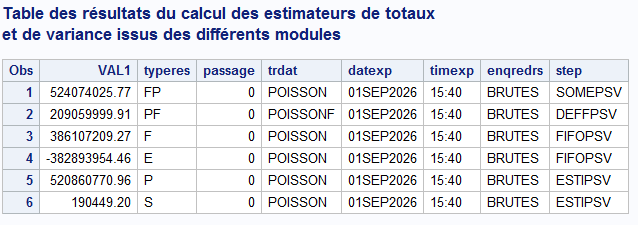
\includegraphics[width=0.9\linewidth]{figures/Poulpe_SRS_NR} \end{center}

In \texttt{Poulpe}, the non-response variance component is not displayed
directly. Instead, \texttt{Poulpe} outputs two intermediate quantities,
F and E, whose difference yields the non-response variance (see Caron,
1998, p. 185). Understanding the relationship between these quantities
and the \texttt{gustave} formulation requires examining how the Poisson
variance formula is parameterised.

\begin{table}[t]
\caption{\label{tab:unnamed-chunk-11}Variance elements for Poulpe calculated from gustave} 
\fontsize{12.0pt}{14.0pt}\selectfont
\begin{tabular*}{\linewidth}{@{\extracolsep{\fill}}lllr}
\toprule
Component & typeres & gustave & value \\ 
\midrule\addlinespace[2.5pt]
Point estimate & S & est & 190449.2 \\ 
Sampling variance & P & `var\_srs()` component & 520860771.0 \\ 
F-Non-response component & F &  & 386107209.3 \\ 
E-Non-response component & E &  & -382893954.5 \\ 
Non-response variance & E+F & `var\_pois()` component & 3213254.8 \\ 
Total variance & FP & var & 524074025.8 \\ 
\bottomrule
\end{tabular*}
\end{table}

The F component in Poulpe corresponds to a Poisson variance where the
sampling weight has been absorbed into the variable of interest (i.e.,
the formula operates on \(y_i / (\pi_i p_i)\) rather than on \(y_i\)
with a separate weight argument):

\[V_{\text{F-poulpe}} = \sum_{i\in \text{resp}}{(1-p_i) \left(\frac{y_i}{p_i\pi_i}\right)^2}\]

This is obtained in gustave by passing the pre-weighted variable to
\texttt{var\_pois()}: \texttt{var\_pois(y\ /\ pik\_i,\ pik\ =\ p\_i)}.

The \texttt{gustave} non-response variance, by contrast, keeps the
sampling weight separate through the \texttt{w} argument:

\[V_{\text{NR}} = \sum_{i\in \text{resp}}{ \frac{1}{\pi_i} (1-p_i) \left(\frac{y_i}{p_i}\right)^2}\]

The difference between these two expressions is the E component:

\[V_{\text{E-poulpe}} = V_{\text{NR}} - V_{\text{F-poulpe}} = \sum_{i\in \text{resp}}{(1-p_i) \left(\frac{y_i}{p_i}\right)^2 \left(\frac{1}{\pi_i} - \frac{1}{\pi_i^2}\right)}\]

The E-part of the Poulpe calculation is negative and can be obtained by
setting \(\text{var\_pois}(y_i,p_i,1/\pi - 1/\pi^2)\). This component is
not a variance in itself, it is an intermediate result. The meaningful
quantity is always \(E + F\), which equals the \texttt{gustave}
non-response component. In practice, verifying that the \texttt{gustave}
total variance (FP) matches the \texttt{Poulpe} output is sufficient;
the F and E components are useful for debugging but carry no independent
methodological interpretation.

\section{Case 3: Adding Calibration}\label{case-3-adding-calibration}

\subsection{Context}\label{context-2}

Here we account for \textbf{calibration} in the variance estimation.
After non-response correction, the weights are typically calibrated on
known population margins (e.g., totals by region, by sex, by age group)
to reduce bias and improve precision.

Calibration reduces the variance of the estimator: by forcing the
weighted sample to reproduce known population totals, it removes part of
the variability.

\subsection{Variance decomposition}\label{variance-decomposition-2}

There is no major change in the formula of variance estimation, we just
need to replace the variable of interest \texttt{y} with
\textbf{calibration residuals} before computing the variance components.
These calibration residuals are obtained as the residuals of a weighted
linear regression of \texttt{y} on the calibration variables \texttt{x}:

\[e_k = y_k - x_k' \hat{\beta}, \quad \text{where} \quad \hat{\beta} = (X'WX)^{-1} X'Wy\]

These residuals capture the part of \texttt{y} that is not explained by
the calibration variables, which is the only part that contributes to
the variance.

\begin{Shaded}
\begin{Highlighting}[]
\NormalTok{resp\_dwel }\OtherTok{\textless{}{-}}\NormalTok{ lfs\_samp\_dwel }\SpecialCharTok{\%\textgreater{}\%} \FunctionTok{filter}\NormalTok{(rep }\SpecialCharTok{==} \DecValTok{1}\NormalTok{)}

\CommentTok{\# Example: if calibrating on id\_area (catégorical)}
\NormalTok{e }\OtherTok{\textless{}{-}} \FunctionTok{res\_cal}\NormalTok{(resp\_dwel}\SpecialCharTok{$}\NormalTok{income, }\AttributeTok{x =} \FunctionTok{model.matrix}\NormalTok{(}\SpecialCharTok{\textasciitilde{}}\NormalTok{ id\_area, }\AttributeTok{data =}\NormalTok{ resp\_dwel))}
\end{Highlighting}
\end{Shaded}

\textbf{Important:} \texttt{res\_cal()} by default performs the
regression \textbf{without an intercept}. The example above uses
\texttt{model.matrix()} (intercept + treatment contrasts) instead. In
\texttt{qvar()}, Qualitative calibration variables (character or factor)
are automatically discretized into full sets of dummies.

For all the following cases, we assume the weights have already been
calibrated on the variable \texttt{id\_area}.

\subsection{\texorpdfstring{Using
\texttt{qvar()}}{Using qvar()}}\label{using-qvar-2}

\begin{Shaded}
\begin{Highlighting}[]
\NormalTok{lfs\_samp\_dwel }\OtherTok{\textless{}{-}} \FunctionTok{as.data.frame}\NormalTok{(lfs\_samp\_dwel)}

\NormalTok{precision\_cal }\OtherTok{\textless{}{-}} \FunctionTok{qvar}\NormalTok{(}
  \AttributeTok{data                 =}\NormalTok{ lfs\_samp\_dwel,}
  \AttributeTok{id                   =} \StringTok{"id\_dwel"}\NormalTok{,}
  \AttributeTok{strata               =} \StringTok{"id\_area"}\NormalTok{,}
  \AttributeTok{dissemination\_dummy  =} \StringTok{"rep"}\NormalTok{,}
  \AttributeTok{dissemination\_weight =} \StringTok{"w\_final\_nrc"}\NormalTok{,}
  \AttributeTok{sampling\_weight      =} \StringTok{"w\_final"}\NormalTok{,}
  \AttributeTok{nrc\_weight           =} \StringTok{"w\_final\_nrc"}\NormalTok{,}
  \AttributeTok{response\_dummy       =} \StringTok{"rep"}\NormalTok{,}
  \AttributeTok{calibration\_dummy    =} \StringTok{"rep"}\NormalTok{,}
  \AttributeTok{calibration\_weight   =} \StringTok{"w\_final\_nrc"}\NormalTok{,}
  \AttributeTok{calibration\_var      =} \StringTok{"id\_area"}\NormalTok{,}
  \AttributeTok{define =} \ConstantTok{TRUE}
\NormalTok{)}
\CommentTok{\#\textgreater{} Survey variance estimation with the gustave package}
\CommentTok{\#\textgreater{} }
\CommentTok{\#\textgreater{} The following features are taken into account:}
\CommentTok{\#\textgreater{}   {-} stratified simple random sampling}
\CommentTok{\#\textgreater{}   {-} non{-}response correction through reweighting}
\CommentTok{\#\textgreater{}   {-} calibration on margins}
\CommentTok{\#\textgreater{} Note: The strata variable (id\_area) is of type character. It is automatically coerced to factor.}
\CommentTok{\#\textgreater{} Note: Note: The following calibration variables are qualitative (factor, character): id\_area. They will be automatically discretized.}
\CommentTok{\#\textgreater{} Note: As define = TRUE, a ready{-}to{-}use variance wrapper is (invisibly) returned.}

\FunctionTok{precision\_cal}\NormalTok{(lfs\_samp\_dwel, }\FunctionTok{total}\NormalTok{(income))}
\CommentTok{\#\textgreater{} Warning: 32 observations do not match any responding units of the survey. They are discarded.}
\CommentTok{\#\textgreater{}                call  n      est  variance     std       cv    lower    upper}
\CommentTok{\#\textgreater{} 1 total(y = income) 48 190449.2 197245302 14044.4 7.374359 162922.6 217975.7}
\end{Highlighting}
\end{Shaded}

New arguments:

\begin{itemize}
\tightlist
\item
  \texttt{calibration\_dummy}: which units were used in the calibration
  (typically, the respondents).
\item
  \texttt{calibration\_weight}: the calibrated weight.
\item
  \texttt{calibration\_var}: the calibration variable(s). For
  categorical variables, \texttt{qvar()} automatically creates the dummy
  matrix.
\end{itemize}

\textbf{Note:} \texttt{qvar()} does not accept tibbles when calibration
variables are specified. Convert to \texttt{data.frame} first.

\subsection{\texorpdfstring{Using
\texttt{define\_variance\_wrapper()}}{Using define\_variance\_wrapper()}}\label{using-define_variance_wrapper-2}

\subsubsection{Variance function}\label{variance-function-2}

The variance function now includes a \texttt{res\_cal()} step before the
variance components:

\begin{Shaded}
\begin{Highlighting}[]
\NormalTok{diag\_env }\OtherTok{\textless{}{-}} \FunctionTok{new.env}\NormalTok{(}\AttributeTok{parent =} \FunctionTok{emptyenv}\NormalTok{())}

\NormalTok{var\_sample\_cal }\OtherTok{\textless{}{-}} \ControlFlowTok{function}\NormalTok{(y, lfs\_samp\_dwel) \{}
  
\NormalTok{  variance }\OtherTok{\textless{}{-}} \FunctionTok{list}\NormalTok{()}

\NormalTok{  resp }\OtherTok{\textless{}{-}}\NormalTok{ lfs\_samp\_dwel }\SpecialCharTok{\%\textgreater{}\%} \FunctionTok{filter}\NormalTok{(rep }\SpecialCharTok{==} \DecValTok{1}\NormalTok{)}
  
  \CommentTok{\# Step 0: Prepare the calibration matrix (respondents only)}
\NormalTok{  cal\_form }\OtherTok{\textless{}{-}} \FunctionTok{as.formula}\NormalTok{(}\StringTok{"\textasciitilde{}id\_area"}\NormalTok{)}
\NormalTok{  x\_cal }\OtherTok{\textless{}{-}} \FunctionTok{model.matrix}\NormalTok{(cal\_form, }\AttributeTok{data =}\NormalTok{ resp)}

  \CommentTok{\# Step 1: Replace y with calibration residuals (respondents only)}
\NormalTok{  y[resp}\SpecialCharTok{$}\NormalTok{id\_dwel, ] }\OtherTok{\textless{}{-}} \FunctionTok{res\_cal}\NormalTok{(}
\NormalTok{    y[resp}\SpecialCharTok{$}\NormalTok{id\_dwel, ,}\AttributeTok{drop =} \ConstantTok{FALSE}\NormalTok{],}
    \AttributeTok{x =}\NormalTok{ x\_cal,}
    \AttributeTok{w =}\NormalTok{ resp}\SpecialCharTok{$}\NormalTok{w\_final\_nrc}
\NormalTok{  )}
  
  \CommentTok{\# Step 2: Non{-}response variance (Poisson, respondents only)}
\NormalTok{  variance[[}\StringTok{"nr"}\NormalTok{]] }\OtherTok{\textless{}{-}} \FunctionTok{var\_pois}\NormalTok{(}
\NormalTok{    y[resp}\SpecialCharTok{$}\NormalTok{id\_dwel, ,}\AttributeTok{drop =} \ConstantTok{FALSE}\NormalTok{],}
    \AttributeTok{pik =}\NormalTok{ resp}\SpecialCharTok{$}\NormalTok{prep,}
    \AttributeTok{w   =}\NormalTok{ resp}\SpecialCharTok{$}\NormalTok{w\_final}
\NormalTok{  )}
  
\NormalTok{  poulpe\_F }\OtherTok{\textless{}{-}} \FunctionTok{var\_pois}\NormalTok{(}
\NormalTok{    y[resp}\SpecialCharTok{$}\NormalTok{id\_dwel, ,}\AttributeTok{drop =} \ConstantTok{FALSE}\NormalTok{] }\SpecialCharTok{*}\NormalTok{ resp}\SpecialCharTok{$}\NormalTok{w\_final,}
    \AttributeTok{pik =}\NormalTok{ resp}\SpecialCharTok{$}\NormalTok{prep}
\NormalTok{  )}
  
  \CommentTok{\# Step 3: Reintroduce non{-}respondents with zeros}
\NormalTok{  y }\OtherTok{\textless{}{-}} \FunctionTok{add\_zero}\NormalTok{(y, }\AttributeTok{rownames =}\NormalTok{ lfs\_samp\_dwel}\SpecialCharTok{$}\NormalTok{id\_dwel)}
  
  \CommentTok{\# Step 4: Sampling variance (SRS, full sample)}
\NormalTok{  variance[[}\StringTok{"srs"}\NormalTok{]] }\OtherTok{\textless{}{-}} \FunctionTok{var\_srs}\NormalTok{(}
\NormalTok{    y }\SpecialCharTok{/}\NormalTok{ (lfs\_samp\_dwel}\SpecialCharTok{$}\NormalTok{prep),}
    \AttributeTok{pik    =} \DecValTok{1} \SpecialCharTok{/}\NormalTok{ lfs\_samp\_dwel}\SpecialCharTok{$}\NormalTok{w\_final,}
    \AttributeTok{strata =}\NormalTok{ lfs\_samp\_dwel}\SpecialCharTok{$}\NormalTok{id\_area}
\NormalTok{  )}
  
\NormalTok{  diag\_env}\SpecialCharTok{$}\NormalTok{components }\OtherTok{\textless{}{-}}\NormalTok{ variance}
\NormalTok{  diag\_env}\SpecialCharTok{$}\NormalTok{poulpe }\OtherTok{\textless{}{-}} \FunctionTok{tibble}\NormalTok{(}\AttributeTok{typeres=}\StringTok{"FP"}\NormalTok{,}\AttributeTok{value=}\FunctionTok{Reduce}\NormalTok{(}\StringTok{\textasciigrave{}}\AttributeTok{+}\StringTok{\textasciigrave{}}\NormalTok{, variance)) }\SpecialCharTok{\%\textgreater{}\%}
    \FunctionTok{add\_row}\NormalTok{(}\AttributeTok{typeres=}\StringTok{"PF"}\NormalTok{,}\AttributeTok{value=}\ConstantTok{NA}\NormalTok{) }\SpecialCharTok{\%\textgreater{}\%} 
    \FunctionTok{add\_row}\NormalTok{(}\AttributeTok{typeres=}\StringTok{"F"}\NormalTok{,}\AttributeTok{value=}\NormalTok{poulpe\_F) }\SpecialCharTok{\%\textgreater{}\%} 
    \FunctionTok{add\_row}\NormalTok{(}\AttributeTok{typeres=}\StringTok{"E"}\NormalTok{,}\AttributeTok{value=}\NormalTok{variance[[}\StringTok{"nr"}\NormalTok{]] }\SpecialCharTok{{-}}\NormalTok{ poulpe\_F) }\SpecialCharTok{\%\textgreater{}\%} 
    \FunctionTok{add\_row}\NormalTok{(}\AttributeTok{typeres=}\StringTok{"P"}\NormalTok{,}\AttributeTok{value=}\NormalTok{variance[[}\StringTok{"srs"}\NormalTok{]]) }\SpecialCharTok{\%\textgreater{}\%} 
    \FunctionTok{add\_row}\NormalTok{(}\AttributeTok{typeres=}\StringTok{"S"}\NormalTok{,}\AttributeTok{value=}\ConstantTok{NA}\NormalTok{) }
  
  \FunctionTok{Reduce}\NormalTok{(}\StringTok{\textasciigrave{}}\AttributeTok{+}\StringTok{\textasciigrave{}}\NormalTok{, variance)}
\NormalTok{\}}
\end{Highlighting}
\end{Shaded}

The key addition is \textbf{Step 1}: before any variance computation, we
replace \texttt{y} with its calibration residuals. This reduces the
variance because the part of \texttt{y} explained by the calibration
variables is removed.

Here, we have hardcoded the calibration variables in the variance
function itself. In practice, it is better to dynamically build the
calibration matrix from all variables in \texttt{lfs\_samp\_dwel} used
in the calibration model. We will see in the Practical Implementation
section how to make the calibration variables fully configurable through
the \texttt{technical\_data} and \texttt{technical\_param} mechanism, so
that the same variance function can accommodate different calibration
specifications without modifying its source code.

\subsubsection{Technical data and wrapper
creation}\label{technical-data-and-wrapper-creation-1}

The creation of the wrapper is unchanged.

\begin{Shaded}
\begin{Highlighting}[]
\NormalTok{technical\_data\_cal }\OtherTok{\textless{}{-}} \FunctionTok{list}\NormalTok{()}
\NormalTok{technical\_data\_cal}\SpecialCharTok{$}\NormalTok{lfs\_samp\_dwel }\OtherTok{\textless{}{-}}\NormalTok{ lfs\_samp\_dwel}

\NormalTok{precision2\_cal }\OtherTok{\textless{}{-}} \FunctionTok{define\_variance\_wrapper}\NormalTok{(}
  \AttributeTok{variance\_function =}\NormalTok{ var\_sample\_cal,}
  \AttributeTok{technical\_data    =}\NormalTok{ technical\_data\_cal,}
  \AttributeTok{reference\_id      =}\NormalTok{ technical\_data\_cal}\SpecialCharTok{$}\NormalTok{lfs\_samp\_dwel}\SpecialCharTok{$}\NormalTok{id\_dwel,}
  \AttributeTok{reference\_weight  =}\NormalTok{ technical\_data\_cal}\SpecialCharTok{$}\NormalTok{lfs\_samp\_dwel}\SpecialCharTok{$}\NormalTok{w\_final\_nrc,}
  \AttributeTok{default\_id        =} \StringTok{"id\_dwel"}
\NormalTok{)}
\end{Highlighting}
\end{Shaded}

\subsubsection{Using the wrapper}\label{using-the-wrapper-2}

We expect a lower variance estimation with calibration step.

\begin{Shaded}
\begin{Highlighting}[]
\FunctionTok{precision2}\NormalTok{(lfs\_samp\_dwel, }\FunctionTok{total}\NormalTok{(income))}
\CommentTok{\#\textgreater{}                call  n      est  variance      std       cv    lower    upper}
\CommentTok{\#\textgreater{} 1 total(y = income) 80 114269.5 187509878 13693.42 11.98345 87430.87 141108.1}
\FunctionTok{precision\_nrc}\NormalTok{(lfs\_samp\_dwel, }\FunctionTok{total}\NormalTok{(income))}
\CommentTok{\#\textgreater{} Warning: 32 observations do not match any responding units of the survey. They are discarded.}
\CommentTok{\#\textgreater{}                call  n      est  variance      std       cv    lower  upper}
\CommentTok{\#\textgreater{} 1 total(y = income) 48 190449.2 524074026 22892.66 12.02035 145580.4 235318}
\NormalTok{(results }\OtherTok{\textless{}{-}} \FunctionTok{precision2\_cal}\NormalTok{(lfs\_samp\_dwel, }\FunctionTok{total}\NormalTok{(income)))}
\CommentTok{\#\textgreater{}                call  n      est  variance     std       cv    lower    upper}
\CommentTok{\#\textgreater{} 1 total(y = income) 80 190449.2 197245302 14044.4 7.374359 162922.6 217975.7}
\end{Highlighting}
\end{Shaded}

\subsection{\texorpdfstring{Comparison with
\texttt{Poulpe}}{Comparison with Poulpe}}\label{comparison-with-poulpe-1}

Here is the variance calculated by \texttt{Poulpe} :

\begin{center}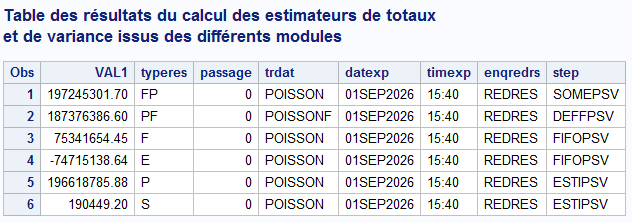
\includegraphics[width=0.9\linewidth]{figures/Poulpe_SRS_NR_CAL} \end{center}

\begin{table}[t]
\caption{\label{tab:unnamed-chunk-14}Variance elements for Poulpe calculated from gustave} 
\fontsize{12.0pt}{14.0pt}\selectfont
\begin{tabular*}{\linewidth}{@{\extracolsep{\fill}}lllr}
\toprule
Component & typeres & gustave & value \\ 
\midrule\addlinespace[2.5pt]
Point estimate & S & est & 190449.2 \\ 
Sampling variance & P & `var\_srs()` component & 196618785.9 \\ 
F-Non-response component & F &  & 75341654.5 \\ 
E-Non-response component & E &  & -74715138.6 \\ 
Non-response variance & E+F & `var\_pois()` component & 626515.8 \\ 
? & PF & ? & NA \\ 
Total variance & FP & var & 197245301.7 \\ 
\bottomrule
\end{tabular*}
\end{table}

\section{Case 4: Two-Stage Sampling}\label{case-4-two-stage-sampling}

\subsection{Context}\label{context-3}

In many dwelling surveys at Statbel (such as LFS), the sampling design
involves two stages. First, a random sample of municipalities is drawn
from the population. Then a stratified random sample of dwellings is
drawn. Some of them do not respond, and answers are at dwelling level.
At last, weights are corrected through reweighting.

\subsection{Variance decomposition}\label{variance-decomposition-3}

This two-stage design introduces an additional source of variability
compared to the previous cases. The total variance now decomposes into
three additive components:

\[V(\hat{Y})=V_{PSU}+V_{HH}+V_{NR}\]

The first component captures the uncertainty from drawing PSUs from the
population. The second captures the uncertainty from drawing dwellings
from the selected PSU. The last component accounts for the random nature
of dwelling non-response.

Let us define the following quantities. At the PSU level: \(N_P\) is the
total number of PSUs in the population, \(n_P\) is the number of sampled
PSUs, and \(\pi_{\text{psu}}\) is the first-order inclusion probability
of a PSU. At the dwelling level: \(N_{h|j}\) is the number of dwellings
in PSU \(j\) for the strata \(h\), \(n_{h|j}\) is the number of sampled
dwellings in PSU \(j\) for the strata \(h\), and \(\pi_{h|j}\) is the
conditional inclusion probability of dwelling \(h\) given that PSU \(j\)
and strata \(h\) has been selected. The overall inclusion probability of
a dwelling is
\(\pi_h = \pi_{\text{psu}(h)} \cdot \pi_{h|\text{psu}(h)}\). Finally,
\(p_h\) denotes the estimated response probability for dwelling \(h\).

Non-response is modeled as a Poisson sampling phase. For each responding
dwelling, the contribution to the non-response variance depends on its
response probability and its fully expanded value. The formula is:

\[V_{\text{NR}} = \sum_{i\in \text{resp}}{ \frac{1}{\pi_i} (1-p_i) \left(\frac{y_i}{p_i}\right)^2}\]

Within each selected PSU, a simple random sample of dwellings is drawn.
The sub-sampling variance is the sum, across all sampled PSUs, of the
within-PSU SRS variance, each weighted by the inverse of the PSU
inclusion probability to account for the fact that only a fraction of
the PSUs are observed:

\[V_{HH} = \sum_{j=1}^{n_P}{\frac{1}{\pi_{\text{psu},j}} \left[ \sum_{h=1}^{H} N_{h|j}^2 \left(1 - \frac{n_{h|j}}{N_{h|j}}\right) \frac{s_{h|j}^2}{n_{h|j}} \right]}\]

where \(s_{h|j}^2\) is the sample variance of the non-response-corrected
variable \(y_h / p_h\) within PSU \(j\). In the R code, this is
implemented by looping over PSUs and calling \texttt{var\_srs()} on each
subset, then multiplying by \(1/\pi_{\text{psu}}\).

Before computing the PSU-level variance, the dwelling-level variable
must be aggregated to PSU totals. For each PSU \(j\), the estimated PSU
total is obtained by expanding the non-response-corrected dwelling
values using the within-PSU Horvitz-Thompson estimator:

\[\hat Y_{j} = \sum_{h\in j} \frac{1}{\pi_{h|j}}\frac{y_{h}}{p_h}\]

In \texttt{gustave}, this aggregation is performed by \texttt{sum\_by()}
with the weight argument set to \(1/{\pi_{h|j}}\).

Once the PSU-level totals \(\hat Y_{j}\) are available, the PSU sampling
variance follows the standard stratified SRS formula:

\[V_{PSU} = N_{P}^2 \left( 1 - \frac{n_{P}}{N_{P}} \right)\frac{s^2_{P}}{n_{P}}\]

Where \(s^2_{P}\) is the sample variance of the \(\hat Y_{j}\) values.
In \texttt{gustave}, this is a single call to \texttt{var\_srs()}.

This case cannot be handled by \texttt{qvar()}, which is limited to
single-stage designs. It is precisely the kind of situation where
\texttt{define\_variance\_wrapper()} becomes essential: we need to write
a custom variance function that chains the three components in the
correct order --- from the innermost stage (dwelling sub-sampling) back
to the outermost stage (PSU sampling), applying \texttt{add\_zero()} at
each transition to reintroduce the units lost at the previous step.

We explain step by step the \texttt{define\_variance\_wrapper()}
writing, then we introduce a custom \texttt{qvar\_ms()} function, to
estimate variance for multi-levels stratified simple random sampling.

For this case, we use the two datasets \texttt{lfs\_samp\_area} and
\texttt{lfs\_samp\_dwel}.

\subsection{\texorpdfstring{Using
\texttt{define\_variance\_wrapper()}}{Using define\_variance\_wrapper()}}\label{using-define_variance_wrapper-3}

\subsubsection{Variance function}\label{variance-function-3}

\begin{Shaded}
\begin{Highlighting}[]
\NormalTok{diag\_env }\OtherTok{\textless{}{-}} \FunctionTok{new.env}\NormalTok{(}\AttributeTok{parent =} \FunctionTok{emptyenv}\NormalTok{())}
\NormalTok{var\_sample\_two }\OtherTok{\textless{}{-}} \ControlFlowTok{function}\NormalTok{(y, lfs\_samp\_area, lfs\_samp\_dwel) \{}
  
\NormalTok{  variance }\OtherTok{\textless{}{-}} \FunctionTok{list}\NormalTok{()}

  \CommentTok{\# Step 0: Prepare the respondents datasets}
\NormalTok{  resp\_dwel }\OtherTok{\textless{}{-}}\NormalTok{ lfs\_samp\_dwel }\SpecialCharTok{\%\textgreater{}\%} \FunctionTok{filter}\NormalTok{(rep }\SpecialCharTok{==} \DecValTok{1}\NormalTok{)}
  
  \CommentTok{\# Step 1: Prepare the calibration matrix (individual level)}
\NormalTok{  cal\_form }\OtherTok{\textless{}{-}} \FunctionTok{as.formula}\NormalTok{(}\StringTok{"\textasciitilde{}id\_area"}\NormalTok{)}
\NormalTok{  x\_cal }\OtherTok{\textless{}{-}} \FunctionTok{model.matrix}\NormalTok{(cal\_form, }\AttributeTok{data =}\NormalTok{ resp\_dwel)}

  \CommentTok{\# Step 2: Replace y with calibration residuals}
\NormalTok{  y[resp\_dwel}\SpecialCharTok{$}\NormalTok{id\_dwel, ] }\OtherTok{\textless{}{-}} \FunctionTok{res\_cal}\NormalTok{(}
\NormalTok{    y[resp\_dwel}\SpecialCharTok{$}\NormalTok{id\_dwel,],}
    \AttributeTok{x =}\NormalTok{ x\_cal,}
    \AttributeTok{w =}\NormalTok{ resp\_dwel}\SpecialCharTok{$}\NormalTok{w\_final\_nrc}
\NormalTok{  )}
  
  \CommentTok{\# Step 3: Non{-}response variance (Poisson, individuals respondents only)}
\NormalTok{  variance[[}\StringTok{"nr"}\NormalTok{]] }\OtherTok{\textless{}{-}} \FunctionTok{var\_pois}\NormalTok{(}
\NormalTok{    y[resp\_dwel}\SpecialCharTok{$}\NormalTok{id\_dwel, ,}\AttributeTok{drop =} \ConstantTok{FALSE}\NormalTok{],}
    \AttributeTok{pik =}\NormalTok{ resp\_dwel}\SpecialCharTok{$}\NormalTok{prep,}
    \AttributeTok{w =}\NormalTok{ resp\_dwel}\SpecialCharTok{$}\NormalTok{w\_final}
\NormalTok{  )}
  
\NormalTok{  poulpe\_F }\OtherTok{\textless{}{-}} \FunctionTok{var\_pois}\NormalTok{(}
\NormalTok{    y[resp\_dwel}\SpecialCharTok{$}\NormalTok{id\_dwel, ,}\AttributeTok{drop =} \ConstantTok{FALSE}\NormalTok{] }\SpecialCharTok{*}\NormalTok{ resp\_dwel}\SpecialCharTok{$}\NormalTok{w\_final,}
    \AttributeTok{pik =}\NormalTok{ resp\_dwel}\SpecialCharTok{$}\NormalTok{prep}
\NormalTok{  )}
  
  \CommentTok{\# Step 4: Reintroduce dwellings non{-}respondents with zeros}
\NormalTok{  y }\OtherTok{\textless{}{-}} \FunctionTok{add\_zero}\NormalTok{(y, }\AttributeTok{rownames =}\NormalTok{ lfs\_samp\_dwel}\SpecialCharTok{$}\NormalTok{id\_dwel)}
  
  \CommentTok{\# Step 5: One variance per PSU, weighted by PSU size}
\NormalTok{  variance[[}\StringTok{"srs{-}dwel"}\NormalTok{]] }\OtherTok{\textless{}{-}} \FunctionTok{unique}\NormalTok{(lfs\_samp\_dwel}\SpecialCharTok{$}\NormalTok{id\_area) }\SpecialCharTok{\%\textgreater{}\%} \FunctionTok{map}\NormalTok{(}\SpecialCharTok{\textasciitilde{}}\NormalTok{\{}
\NormalTok{    sub }\OtherTok{\textless{}{-}}\NormalTok{ lfs\_samp\_dwel }\SpecialCharTok{\%\textgreater{}\%} \FunctionTok{filter}\NormalTok{(id\_area }\SpecialCharTok{==}\NormalTok{ .x)}
\NormalTok{    pik\_area }\OtherTok{\textless{}{-}} \DecValTok{1} \SpecialCharTok{/} \FunctionTok{unique}\NormalTok{(sub}\SpecialCharTok{$}\NormalTok{w\_area)}
    \FunctionTok{var\_srs}\NormalTok{(}
\NormalTok{      y[sub}\SpecialCharTok{$}\NormalTok{id\_dwel, ,}\AttributeTok{drop =} \ConstantTok{FALSE}\NormalTok{] }\SpecialCharTok{/}\NormalTok{ sub}\SpecialCharTok{$}\NormalTok{prep,}
      \AttributeTok{pik    =} \DecValTok{1} \SpecialCharTok{/}\NormalTok{ sub}\SpecialCharTok{$}\NormalTok{w\_dwel}
\NormalTok{    ) }\SpecialCharTok{*} \DecValTok{1}\SpecialCharTok{/}\NormalTok{pik\_area}
\NormalTok{  \}) }\SpecialCharTok{\%\textgreater{}\%}\NormalTok{ unlist }\SpecialCharTok{\%\textgreater{}\%}\NormalTok{ sum}
  
  \CommentTok{\# {-}{-}{-} Transition: aggregate to area level {-}{-}{-}}
\NormalTok{  y\_area }\OtherTok{\textless{}{-}} \FunctionTok{sum\_by}\NormalTok{(y }\SpecialCharTok{/}\NormalTok{ lfs\_samp\_dwel}\SpecialCharTok{$}\NormalTok{prep, }
                   \AttributeTok{by =}\NormalTok{ lfs\_samp\_dwel}\SpecialCharTok{$}\NormalTok{id\_area, }
                   \AttributeTok{w =}\NormalTok{ lfs\_samp\_dwel}\SpecialCharTok{$}\NormalTok{w\_dwel)}
  
  \CommentTok{\# Step 6: area sampling variance}
\NormalTok{  variance[[}\StringTok{"srs{-}area"}\NormalTok{]] }\OtherTok{\textless{}{-}} \FunctionTok{var\_srs}\NormalTok{(}
\NormalTok{    y\_area[lfs\_samp\_area}\SpecialCharTok{$}\NormalTok{id\_area, , }\AttributeTok{drop =} \ConstantTok{FALSE}\NormalTok{],}
    \AttributeTok{pik    =} \DecValTok{1} \SpecialCharTok{/}\NormalTok{ lfs\_samp\_area}\SpecialCharTok{$}\NormalTok{w\_area}
\NormalTok{  )}
  
\NormalTok{  diag\_env}\SpecialCharTok{$}\NormalTok{components }\OtherTok{\textless{}{-}}\NormalTok{ variance}
\NormalTok{  diag\_env}\SpecialCharTok{$}\NormalTok{poulpe }\OtherTok{\textless{}{-}} \FunctionTok{tibble}\NormalTok{(}\AttributeTok{typeres=}\StringTok{"FP"}\NormalTok{,}\AttributeTok{value=}\FunctionTok{Reduce}\NormalTok{(}\StringTok{\textasciigrave{}}\AttributeTok{+}\StringTok{\textasciigrave{}}\NormalTok{, variance)) }\SpecialCharTok{\%\textgreater{}\%}
    \FunctionTok{add\_row}\NormalTok{(}\AttributeTok{typeres=}\StringTok{"PF"}\NormalTok{,}\AttributeTok{value=}\ConstantTok{NA}\NormalTok{) }\SpecialCharTok{\%\textgreater{}\%} 
    \FunctionTok{add\_row}\NormalTok{(}\AttributeTok{typeres=}\StringTok{"F"}\NormalTok{,}\AttributeTok{value=}\NormalTok{poulpe\_F) }\SpecialCharTok{\%\textgreater{}\%} 
    \FunctionTok{add\_row}\NormalTok{(}\AttributeTok{typeres=}\StringTok{"E"}\NormalTok{,}\AttributeTok{value=}\NormalTok{variance[[}\StringTok{"nr"}\NormalTok{]] }\SpecialCharTok{{-}}\NormalTok{ poulpe\_F) }\SpecialCharTok{\%\textgreater{}\%} 
    \FunctionTok{add\_row}\NormalTok{(}\AttributeTok{typeres=}\StringTok{"P"}\NormalTok{,}\AttributeTok{value=}\NormalTok{variance[[}\StringTok{"srs{-}dwel"}\NormalTok{]] }\SpecialCharTok{+}\NormalTok{ variance[[}\StringTok{"srs{-}area"}\NormalTok{]]) }\SpecialCharTok{\%\textgreater{}\%} 
    \FunctionTok{add\_row}\NormalTok{(}\AttributeTok{typeres=}\StringTok{"S"}\NormalTok{,}\AttributeTok{value=}\ConstantTok{NA}\NormalTok{)}
  
  \FunctionTok{Reduce}\NormalTok{(}\StringTok{\textasciigrave{}}\AttributeTok{+}\StringTok{\textasciigrave{}}\NormalTok{, variance)}
\NormalTok{\}}
\end{Highlighting}
\end{Shaded}

The key addition is two aggregations, one at dwelling then at area
level. The calibration is done at individual level. There are two
\texttt{var\_srs()} steps, the key step here is to estimate variance of
dwelling within each area, and then to divide by the selection
probability of each area After that, we aggregate from dwelling to area
with the non-response correction and finally calculate the variance due
to the area sampling.

\subsubsection{Technical data and
Wrapper}\label{technical-data-and-wrapper}

\begin{Shaded}
\begin{Highlighting}[]
\NormalTok{technical\_data\_two }\OtherTok{\textless{}{-}} \FunctionTok{list}\NormalTok{()}
\NormalTok{technical\_data\_two}\SpecialCharTok{$}\NormalTok{lfs\_samp\_area }\OtherTok{\textless{}{-}}\NormalTok{ lfs\_samp\_area}
\NormalTok{technical\_data\_two}\SpecialCharTok{$}\NormalTok{lfs\_samp\_dwel  }\OtherTok{\textless{}{-}}\NormalTok{ lfs\_samp\_dwel}

\NormalTok{precision\_two }\OtherTok{\textless{}{-}} \FunctionTok{define\_variance\_wrapper}\NormalTok{(}
  \AttributeTok{variance\_function =}\NormalTok{ var\_sample\_two,}
  \AttributeTok{technical\_data    =}\NormalTok{ technical\_data\_two,}
  \AttributeTok{reference\_id      =}\NormalTok{ technical\_data\_two}\SpecialCharTok{$}\NormalTok{lfs\_samp\_dwel}\SpecialCharTok{$}\NormalTok{id\_dwel,}
  \AttributeTok{reference\_weight  =}\NormalTok{ technical\_data\_two}\SpecialCharTok{$}\NormalTok{lfs\_samp\_dwel}\SpecialCharTok{$}\NormalTok{w\_final\_nrc,}
  \AttributeTok{default\_id        =} \StringTok{"id\_dwel"}
\NormalTok{)}
\end{Highlighting}
\end{Shaded}

\subsubsection{Using the Wrapper}\label{using-the-wrapper-3}

\begin{Shaded}
\begin{Highlighting}[]
\NormalTok{(results }\OtherTok{\textless{}{-}} \FunctionTok{precision\_two}\NormalTok{(lfs\_samp\_dwel }\SpecialCharTok{\%\textgreater{}\%} \FunctionTok{filter}\NormalTok{(rep }\SpecialCharTok{==} \DecValTok{1}\NormalTok{), }\FunctionTok{total}\NormalTok{(income)))}
\CommentTok{\#\textgreater{} Warning: Some observations from the survey appear to be missing. The variance estimation function may produce unexpected results.}
\CommentTok{\#\textgreater{} Warning: The inputted id variable (id argument) appears not to match the reference id variable provided when the variance wrapper was defined: it is reordered and everything should be fine. Issues may nonetheless arise if part of the call is to be evaluated outside of the inputted data.frame (data argument).}
\CommentTok{\#\textgreater{}                call  n      est variance      std       cv    lower    upper}
\CommentTok{\#\textgreater{} 1 total(y = income) 48 190449.2  8933292 2988.861 1.569375 184591.1 196307.2}
\end{Highlighting}
\end{Shaded}

\subsection{\texorpdfstring{Using
\texttt{qvar\_ms()}}{Using qvar\_ms()}}\label{using-qvar_ms}

\texttt{qvar\_ms()} extends \texttt{qvar()} to multistage sampling
designs, that is: stratified simple random sampling at each stage (units
of stage k being drawn within the units of stage k - 1) ; non-response
correction (if any) through reweighting, possibly at each stage ;
calibration (if any) at one given stage.

To use \texttt{qvar\_ms()}, you need, at each stage of sampling, the
conditional sampling weight, the probability of response (if any) and
the calibration weight (if any). Parameters are quite identical as
\texttt{qvar()}, except you need list to declare argument for each
stage.

\begin{Shaded}
\begin{Highlighting}[]
\NormalTok{precision2\_two }\OtherTok{\textless{}{-}} \FunctionTok{qvar\_ms}\NormalTok{(}
  
  \CommentTok{\# One file per stage, from the highest to the lowest}
  \AttributeTok{data =} \FunctionTok{list}\NormalTok{(lfs\_samp\_area, lfs\_samp\_dwel),}
  \AttributeTok{sampling\_stages =} \DecValTok{2}\NormalTok{,}
  \AttributeTok{id =} \FunctionTok{c}\NormalTok{(}\StringTok{"id\_area"}\NormalTok{, }\StringTok{"id\_dwel"}\NormalTok{),}
  \AttributeTok{parent\_id =} \StringTok{"id\_area"}\NormalTok{,}
  
  \CommentTok{\# Dissemination and scope (last stage only)}
  \AttributeTok{dissemination\_dummy =} \StringTok{"rep"}\NormalTok{,}
  \AttributeTok{dissemination\_weight =} \StringTok{"w\_final\_nrc"}\NormalTok{,}
  
  \CommentTok{\# Sampling design (conditional weights)}
  \AttributeTok{sampling\_weight =} \FunctionTok{c}\NormalTok{(}\StringTok{"w\_area"}\NormalTok{, }\StringTok{"w\_dwel"}\NormalTok{),}
  
  \CommentTok{\# Non{-}response correction (last stage by default)}
  \AttributeTok{response\_prob =} \StringTok{"prep"}\NormalTok{,}
  \AttributeTok{response\_dummy =} \StringTok{"rep"}\NormalTok{,}

  \CommentTok{\# Calibration (last stage by default, cumulated weight)}
  \AttributeTok{calibration\_weight =} \StringTok{"w\_final\_nrc"}\NormalTok{,}
  \AttributeTok{calibration\_var =} \StringTok{"id\_area"}\NormalTok{,}
  
  \AttributeTok{define =} \ConstantTok{TRUE}
\NormalTok{)}
\CommentTok{\#\textgreater{} Note: The response\_prob argument is of length 1: it is assumed to refer to the last sampling stage (stage 2).}
\CommentTok{\#\textgreater{} Note: The response\_dummy argument is of length 1: it is assumed to refer to the last sampling stage (stage 2).}
\CommentTok{\#\textgreater{} Survey variance estimation with the gustave package}
\CommentTok{\#\textgreater{} }
\CommentTok{\#\textgreater{} The following features are taken into account:}
\CommentTok{\#\textgreater{}   {-} 2{-}stage sampling design}
\CommentTok{\#\textgreater{}   {-} stage 1: simple random sampling WITHOUT stratification}
\CommentTok{\#\textgreater{}   {-} stage 2: simple random sampling WITHOUT stratification (within the units of the stage above), with non{-}response correction through reweighting}
\CommentTok{\#\textgreater{}   {-} calibration on margins at stage 2}
\CommentTok{\#\textgreater{} Note: The following calibration variables are qualitative (factor, character): id\_area. They will be automatically discretized.}
\CommentTok{\#\textgreater{} Note: At stage 2, units are drawn within the units of the stage above: the effective strata used for variance estimation are the crossing of the parent unit (id\_area).}
\CommentTok{\#\textgreater{} Note: As define = TRUE, a ready{-}to{-}use variance wrapper is (invisibly) returned.}

\FunctionTok{precision2\_two}\NormalTok{(lfs\_samp\_dwel,}\FunctionTok{total}\NormalTok{(income))}
\CommentTok{\#\textgreater{} Warning: 32 observations do not match any responding units of the survey. They are discarded.}
\CommentTok{\#\textgreater{}                call  n      est variance      std       cv    lower    upper}
\CommentTok{\#\textgreater{} 1 total(y = income) 48 190449.2  8933292 2988.861 1.569375 184591.1 196307.2}
\end{Highlighting}
\end{Shaded}

\subsection{\texorpdfstring{Comparison with
\texttt{Poulpe}}{Comparison with Poulpe}}\label{comparison-with-poulpe-2}

Here is the variance calculated by \texttt{Poulpe} :

\begin{center}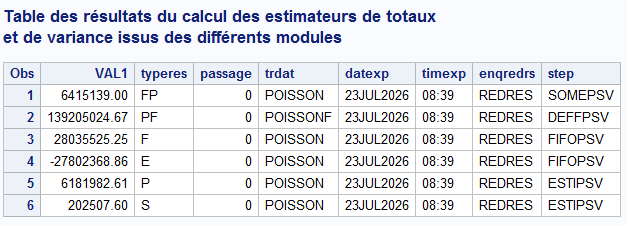
\includegraphics[width=0.9\linewidth]{figures/Poulpe_SRS_NR_CAL_TWO} \end{center}

\begin{table}[t]
\caption{\label{tab:unnamed-chunk-19}Variance elements for Poulpe calculated from gustave} 
\fontsize{12.0pt}{14.0pt}\selectfont
\begin{tabular*}{\linewidth}{@{\extracolsep{\fill}}lllr}
\toprule
Component & typeres & gustave & value \\ 
\midrule\addlinespace[2.5pt]
Point estimate & S & est & 190449.2 \\ 
Sampling variance & P & `var\_srs()` component & 8306775.9 \\ 
F-Non-response component & F &  & 75341654.5 \\ 
E-Non-response component & E &  & -74715138.6 \\ 
Non-response variance & E+F & `var\_pois()` component & 626515.8 \\ 
? & PF & ? & NA \\ 
Total variance & FP & var & 8933291.8 \\ 
\bottomrule
\end{tabular*}
\end{table}

\section{Case 5: Adding individuals
answers}\label{case-5-adding-individuals-answers}

\subsection{Context}\label{context-4}

Case 4 assumed that the variable of interest was measured at the
dwelling level. In practice, however, most survey statistics are
produced at the individual level --- for instance, unemployment rates or
average income per person. In this case, the sampling design remains a
two-stage draw (area sampling, then dwelling SRS within areas), followed
by an exhaustive collection of all individuals within responding
dwellings. The third sampling stage is exhaustive : once a dwelling
responds, all its members are observed.

Once again, \texttt{qvar()} cannot estimate variance for a three-stage
sampling design. We need to develop a variance wrapper by ourself.
\texttt{qvar\_ms()} integrate natively this case. As we see in this
section, the introduction of the individual ask some questions about
which stage the non-response and the calibration occur. We explain the
consequences of each choice, present the choice made by \texttt{Poulpe}
and how to use \texttt{qvar\_ms()} here.

\subsection{Variance decomposition}\label{variance-decomposition-4}

The total variance still decomposes into the same three additive
components as in Case 4:

\[V(\hat{Y})=V_{PSU}+V_{HH}+V_{NR}\]

The formulas are identical to those presented in Case 4. The only
difference is operational: the variable of interest \(y_i\) is now
defined at the individual level and must be aggregated to the dwelling
level (by summing within dwellings) before computing the dwelling and
area variance components. This aggregation step occurs naturally through
\texttt{sum\_by()}.

\subsubsection{Non-response level: dwelling or
individual?}\label{non-response-level-dwelling-or-individual}

A subtle but important question arises: at which level should
non-response be modeled? In reality, non-response occurs at the dwelling
level --- when a dwelling refuses to participate, all its members are
lost simultaneously. However, in the \texttt{Poulpe} methodology,
non-response is always treated as the last phase of the sampling design,
which means it is applied at the level of the analysis unit --- here,
the individual.

These two approaches lead to different variance estimates because they
imply different models for the non-response mechanism. When non-response
is modeled at the dwelling level, the response probability \(p_h\) is
the same for all members of dwelling \(h\), and the non-response
variance is computed on dwelling-level aggregates. When non-response is
modeled at the individual level, each individual carries the response
probability of their dwelling, but the Poisson variance formula is
applied to individual-level values --- which implicitly treats each
individual as an independent response unit.

We implement both approaches below. The first version
(\texttt{var\_sample\_three\_1()}) models non-response at the individual
level, consistent with the \texttt{Poulpe} convention. The second
version (\texttt{var\_sample\_three\_2()}) models non-response at the
dwelling level, which better reflects the actual data-generating
process. Comparing the two helps assess the sensitivity of the variance
estimate to this modelling choice and validates the R implementation
against \texttt{Poulpe} reference values.

\subsubsection{Calibration level}\label{calibration-level}

The level at which calibration residuals are computed depends on the
non-response modelling choice.

In the \texttt{Poulpe}-consistent approach (version 1), calibration is
applied at the individual level before any aggregation. The calibration
matrix contains individual-level variables alongside dwelling-level
variables that are simply repeated for each dwelling member. This is
consistent with \texttt{Poulpe}'s convention of applying a single
\texttt{res\_cal()} at the analysis unit level.

In the dwelling-level approach (version 2), the individual variable of
interest is first aggregated to the dwelling level. Calibration is then
applied at the dwelling level. If the actual calibration used both
dwelling margins and individual margins, the individual calibration
variables must be aggregated to the dwelling level --- typically by
summing the dummy indicators within each dwelling --- before being
included in the \texttt{res\_cal()} calibration matrix. This produces a
dwelling-level residual that accounts for both types of margins
simultaneously.

For this case, we use the three datasets \texttt{lfs\_samp\_area},
\texttt{lfs\_samp\_dwel} and \texttt{lfs\_samp\_ind}. We need to make
some changes to the datasets before using them. In particular, we copy
the \texttt{pik\_dwel} into the individual dataset.

\begin{Shaded}
\begin{Highlighting}[]
\NormalTok{lfs\_samp\_ind }\OtherTok{\textless{}{-}}\NormalTok{ lfs\_samp\_ind }\SpecialCharTok{\%\textgreater{}\%} 
  \FunctionTok{select}\NormalTok{(}\SpecialCharTok{{-}}\FunctionTok{any\_of}\NormalTok{(}\FunctionTok{c}\NormalTok{(}\StringTok{"pik\_area"}\NormalTok{,}\StringTok{"w\_area"}\NormalTok{,}\StringTok{"w\_final\_nrc"}\NormalTok{,}\StringTok{"w\_dwel"}\NormalTok{,}
                   \StringTok{"prep"}\NormalTok{,}\StringTok{"rep"}\NormalTok{,}\StringTok{"id\_area"}\NormalTok{))) }\SpecialCharTok{\%\textgreater{}\%} 
  \FunctionTok{left\_join}\NormalTok{(lfs\_samp\_dwel }\SpecialCharTok{\%\textgreater{}\%} 
              \FunctionTok{select}\NormalTok{(id\_dwel,id\_area,rep,prep,w\_final\_nrc,}
\NormalTok{                     w\_dwel),}\AttributeTok{by =} \StringTok{"id\_dwel"}\NormalTok{) }\SpecialCharTok{\%\textgreater{}\%} 
  \FunctionTok{left\_join}\NormalTok{(lfs\_samp\_area }\SpecialCharTok{\%\textgreater{}\%} 
              \FunctionTok{select}\NormalTok{(id\_area,pik\_area,w\_area),}\AttributeTok{by =} \StringTok{"id\_area"}\NormalTok{)}
\end{Highlighting}
\end{Shaded}

\subsection{\texorpdfstring{Using
\texttt{define\_variance\_wrapper()}}{Using define\_variance\_wrapper()}}\label{using-define_variance_wrapper-4}

\subsubsection{Variance function}\label{variance-function-4}

In \texttt{var\_sample\_three\_1()}, \texttt{res\_cal()} and
\texttt{var\_pois()} are done before dwelling aggregation.

\begin{Shaded}
\begin{Highlighting}[]
\NormalTok{diag\_env\_1 }\OtherTok{\textless{}{-}} \FunctionTok{new.env}\NormalTok{(}\AttributeTok{parent =} \FunctionTok{emptyenv}\NormalTok{())}
\NormalTok{var\_sample\_three\_1 }\OtherTok{\textless{}{-}} \ControlFlowTok{function}\NormalTok{(y, lfs\_samp\_area, lfs\_samp\_dwel, lfs\_samp\_ind) \{}
  
\NormalTok{  variance }\OtherTok{\textless{}{-}} \FunctionTok{list}\NormalTok{()}
\NormalTok{  poulpe }\OtherTok{\textless{}{-}} \FunctionTok{list}\NormalTok{()}

  \CommentTok{\# Step 0: Prepare the respondents datasets}
\NormalTok{  resp\_ind  }\OtherTok{\textless{}{-}}\NormalTok{ lfs\_samp\_ind }\SpecialCharTok{\%\textgreater{}\%} \FunctionTok{filter}\NormalTok{(rep }\SpecialCharTok{==} \DecValTok{1}\NormalTok{)}
\NormalTok{  resp\_dwel }\OtherTok{\textless{}{-}}\NormalTok{ lfs\_samp\_dwel }\SpecialCharTok{\%\textgreater{}\%} \FunctionTok{filter}\NormalTok{(rep }\SpecialCharTok{==} \DecValTok{1}\NormalTok{)}
  
  \CommentTok{\# Step 1: Prepare the calibration matrix (individual level)}
\NormalTok{  cal\_form }\OtherTok{\textless{}{-}} \FunctionTok{as.formula}\NormalTok{(}\StringTok{"\textasciitilde{}id\_area"}\NormalTok{)}
\NormalTok{  x\_cal }\OtherTok{\textless{}{-}} \FunctionTok{model.matrix}\NormalTok{(cal\_form, }\AttributeTok{data =}\NormalTok{ resp\_ind)}

  \CommentTok{\# Step 2: Replace y with calibration residuals}
\NormalTok{  y[resp\_ind}\SpecialCharTok{$}\NormalTok{id\_ind, ] }\OtherTok{\textless{}{-}} \FunctionTok{res\_cal}\NormalTok{(}
\NormalTok{    y[resp\_ind}\SpecialCharTok{$}\NormalTok{id\_ind,],}
    \AttributeTok{x =}\NormalTok{ x\_cal,}
    \AttributeTok{w =}\NormalTok{ resp\_ind}\SpecialCharTok{$}\NormalTok{w\_final\_nrc}
\NormalTok{  )}
  
  \CommentTok{\# Step 3: Non{-}response variance (Poisson, individuals respondents only)}
\NormalTok{  variance[[}\StringTok{"nr"}\NormalTok{]] }\OtherTok{\textless{}{-}} \FunctionTok{var\_pois}\NormalTok{(}
\NormalTok{    y[resp\_ind}\SpecialCharTok{$}\NormalTok{id\_ind, ,}\AttributeTok{drop =} \ConstantTok{FALSE}\NormalTok{],}
    \AttributeTok{pik =}\NormalTok{ resp\_ind}\SpecialCharTok{$}\NormalTok{prep,}
    \AttributeTok{w =}\NormalTok{ resp\_ind}\SpecialCharTok{$}\NormalTok{w\_area }\SpecialCharTok{*}\NormalTok{ resp\_ind}\SpecialCharTok{$}\NormalTok{w\_final}
\NormalTok{  )}
  
\NormalTok{  poulpe\_F }\OtherTok{\textless{}{-}} \FunctionTok{var\_pois}\NormalTok{(}
\NormalTok{    y[resp\_ind}\SpecialCharTok{$}\NormalTok{id\_ind, ,}\AttributeTok{drop =} \ConstantTok{FALSE}\NormalTok{] }\SpecialCharTok{*}\NormalTok{ resp\_ind}\SpecialCharTok{$}\NormalTok{w\_area }\SpecialCharTok{*}\NormalTok{ resp\_ind}\SpecialCharTok{$}\NormalTok{w\_dwel,}
    \AttributeTok{pik =}\NormalTok{ resp\_ind}\SpecialCharTok{$}\NormalTok{prep}
\NormalTok{  )}
  
  \CommentTok{\# Step 4: Reintroduce indviduals non{-}respondents with zeros}
\NormalTok{  y }\OtherTok{\textless{}{-}} \FunctionTok{add\_zero}\NormalTok{(y, }\AttributeTok{rownames =}\NormalTok{ lfs\_samp\_ind}\SpecialCharTok{$}\NormalTok{id\_ind)}
  
  \CommentTok{\# {-}{-}{-} Transition: aggregate to dwelling level {-}{-}{-}}
\NormalTok{  y\_dwel }\OtherTok{\textless{}{-}} \FunctionTok{sum\_by}\NormalTok{(y }\SpecialCharTok{/}\NormalTok{ lfs\_samp\_ind}\SpecialCharTok{$}\NormalTok{prep, }\AttributeTok{by =}\NormalTok{ lfs\_samp\_ind}\SpecialCharTok{$}\NormalTok{id\_dwel)}
  
  \CommentTok{\# Step 5: Reintroduce dwellings non{-}respondents with zeros}
\NormalTok{  y\_dwel }\OtherTok{\textless{}{-}} \FunctionTok{add\_zero}\NormalTok{(y\_dwel, }\AttributeTok{rownames =}\NormalTok{ lfs\_samp\_dwel}\SpecialCharTok{$}\NormalTok{id\_dwel)}
  
  \CommentTok{\# Step 6: One variance per area, weighted by area size}
\NormalTok{  variance[[}\StringTok{"srs{-}dwel"}\NormalTok{]] }\OtherTok{\textless{}{-}} \FunctionTok{unique}\NormalTok{(lfs\_samp\_dwel}\SpecialCharTok{$}\NormalTok{id\_area) }\SpecialCharTok{\%\textgreater{}\%} \FunctionTok{map}\NormalTok{(}\SpecialCharTok{\textasciitilde{}}\NormalTok{\{}
\NormalTok{    sub }\OtherTok{\textless{}{-}}\NormalTok{ lfs\_samp\_dwel }\SpecialCharTok{\%\textgreater{}\%} \FunctionTok{filter}\NormalTok{(id\_area }\SpecialCharTok{==}\NormalTok{ .x)}
\NormalTok{    pik\_area }\OtherTok{\textless{}{-}} \DecValTok{1} \SpecialCharTok{/} \FunctionTok{unique}\NormalTok{(sub}\SpecialCharTok{$}\NormalTok{w\_area)}
    \FunctionTok{var\_srs}\NormalTok{(}
\NormalTok{      y\_dwel[sub}\SpecialCharTok{$}\NormalTok{id\_dwel, ,}\AttributeTok{drop =} \ConstantTok{FALSE}\NormalTok{],}
      \AttributeTok{pik =} \DecValTok{1} \SpecialCharTok{/}\NormalTok{ sub}\SpecialCharTok{$}\NormalTok{w\_dwel}
\NormalTok{    ) }\SpecialCharTok{*} \DecValTok{1}\SpecialCharTok{/}\NormalTok{pik\_area}
\NormalTok{  \}) }\SpecialCharTok{\%\textgreater{}\%}\NormalTok{ unlist }\SpecialCharTok{\%\textgreater{}\%}\NormalTok{ sum}
  
  \CommentTok{\# {-}{-}{-} Transition: aggregate to area level {-}{-}{-}}
\NormalTok{  y\_area }\OtherTok{\textless{}{-}} \FunctionTok{sum\_by}\NormalTok{(y\_dwel, }
                   \AttributeTok{by =}\NormalTok{ lfs\_samp\_dwel}\SpecialCharTok{$}\NormalTok{id\_area, }
                   \AttributeTok{w =}\NormalTok{ lfs\_samp\_dwel}\SpecialCharTok{$}\NormalTok{w\_dwel)}
  
  \CommentTok{\# Step 7: area sampling variance}
\NormalTok{  variance[[}\StringTok{"srs{-}area"}\NormalTok{]] }\OtherTok{\textless{}{-}} \FunctionTok{var\_srs}\NormalTok{(}
\NormalTok{    y\_area[lfs\_samp\_area}\SpecialCharTok{$}\NormalTok{id\_area, , }\AttributeTok{drop =} \ConstantTok{FALSE}\NormalTok{],}
    \AttributeTok{pik    =} \DecValTok{1} \SpecialCharTok{/}\NormalTok{ lfs\_samp\_area}\SpecialCharTok{$}\NormalTok{w\_area}
\NormalTok{  )}
  
\NormalTok{  diag\_env\_1}\SpecialCharTok{$}\NormalTok{components }\OtherTok{\textless{}{-}}\NormalTok{ variance}
\NormalTok{  diag\_env\_1}\SpecialCharTok{$}\NormalTok{poulpe }\OtherTok{\textless{}{-}} \FunctionTok{tibble}\NormalTok{(}\AttributeTok{typeres=}\StringTok{"FP"}\NormalTok{,}\AttributeTok{value=}\FunctionTok{Reduce}\NormalTok{(}\StringTok{\textasciigrave{}}\AttributeTok{+}\StringTok{\textasciigrave{}}\NormalTok{, variance)) }\SpecialCharTok{\%\textgreater{}\%}
    \FunctionTok{add\_row}\NormalTok{(}\AttributeTok{typeres=}\StringTok{"PF"}\NormalTok{,}\AttributeTok{value=}\ConstantTok{NA}\NormalTok{) }\SpecialCharTok{\%\textgreater{}\%} 
    \FunctionTok{add\_row}\NormalTok{(}\AttributeTok{typeres=}\StringTok{"F"}\NormalTok{,}\AttributeTok{value=}\NormalTok{poulpe\_F) }\SpecialCharTok{\%\textgreater{}\%} 
    \FunctionTok{add\_row}\NormalTok{(}\AttributeTok{typeres=}\StringTok{"E"}\NormalTok{,}\AttributeTok{value=}\NormalTok{variance[[}\StringTok{"nr"}\NormalTok{]] }\SpecialCharTok{{-}}\NormalTok{ poulpe\_F) }\SpecialCharTok{\%\textgreater{}\%} 
    \FunctionTok{add\_row}\NormalTok{(}\AttributeTok{typeres=}\StringTok{"P"}\NormalTok{,}\AttributeTok{value=}\NormalTok{variance[[}\StringTok{"srs{-}area"}\NormalTok{]] }\SpecialCharTok{+}\NormalTok{ variance[[}\StringTok{"srs{-}dwel"}\NormalTok{]]) }\SpecialCharTok{\%\textgreater{}\%} 
    \FunctionTok{add\_row}\NormalTok{(}\AttributeTok{typeres=}\StringTok{"S"}\NormalTok{,}\AttributeTok{value=}\ConstantTok{NA}\NormalTok{)}
  
  \FunctionTok{Reduce}\NormalTok{(}\StringTok{\textasciigrave{}}\AttributeTok{+}\StringTok{\textasciigrave{}}\NormalTok{, variance)}
\NormalTok{\}}
\end{Highlighting}
\end{Shaded}

In \texttt{var\_sample\_three\_2()}, \texttt{res\_cal()} and
\texttt{var\_pois()} are done after dwelling aggregation.

\begin{Shaded}
\begin{Highlighting}[]
\NormalTok{diag\_env\_2 }\OtherTok{\textless{}{-}} \FunctionTok{new.env}\NormalTok{(}\AttributeTok{parent =} \FunctionTok{emptyenv}\NormalTok{())}
\NormalTok{var\_sample\_three\_2 }\OtherTok{\textless{}{-}} \ControlFlowTok{function}\NormalTok{(y, lfs\_samp\_area, lfs\_samp\_dwel, lfs\_samp\_ind) \{}
  
\NormalTok{  variance }\OtherTok{\textless{}{-}} \FunctionTok{list}\NormalTok{()}
\NormalTok{  poulpe }\OtherTok{\textless{}{-}} \FunctionTok{list}\NormalTok{()}

  \CommentTok{\# Step 0: Prepare the respondents datasets}
\NormalTok{  resp\_ind  }\OtherTok{\textless{}{-}}\NormalTok{ lfs\_samp\_ind }\SpecialCharTok{\%\textgreater{}\%} \FunctionTok{filter}\NormalTok{(rep }\SpecialCharTok{==} \DecValTok{1}\NormalTok{)}
\NormalTok{  resp\_dwel }\OtherTok{\textless{}{-}}\NormalTok{ lfs\_samp\_dwel }\SpecialCharTok{\%\textgreater{}\%} \FunctionTok{filter}\NormalTok{(rep }\SpecialCharTok{==} \DecValTok{1}\NormalTok{)}
  
   \CommentTok{\# {-}{-}{-} Transition: aggregate to dwelling level {-}{-}{-}}
\NormalTok{  y\_dwel }\OtherTok{\textless{}{-}} \FunctionTok{sum\_by}\NormalTok{(y, }\AttributeTok{by =}\NormalTok{ lfs\_samp\_ind}\SpecialCharTok{$}\NormalTok{id\_dwel)}
  
  \CommentTok{\# Step 1: Prepare the calibration matrix (dwelling level)}
\NormalTok{  cal\_form }\OtherTok{\textless{}{-}} \FunctionTok{as.formula}\NormalTok{(}\StringTok{"\textasciitilde{}id\_area"}\NormalTok{)}
\NormalTok{  x\_cal }\OtherTok{\textless{}{-}} \FunctionTok{model.matrix}\NormalTok{(cal\_form, }\AttributeTok{data =}\NormalTok{ resp\_dwel)}
  
  \CommentTok{\# Step 2: Replace y with calibration residuals}
\NormalTok{  y\_dwel[resp\_dwel}\SpecialCharTok{$}\NormalTok{id\_dwel, ] }\OtherTok{\textless{}{-}} \FunctionTok{res\_cal}\NormalTok{(}
\NormalTok{    y\_dwel[resp\_dwel}\SpecialCharTok{$}\NormalTok{id\_dwel,],}
    \AttributeTok{x =}\NormalTok{ x\_cal,}
    \AttributeTok{w =}\NormalTok{ resp\_dwel}\SpecialCharTok{$}\NormalTok{w\_final\_nrc}
\NormalTok{  )}
  
  \CommentTok{\# Step 3: Non{-}response variance (Poisson, dwelling respondents)}
\NormalTok{  variance[[}\StringTok{"nr"}\NormalTok{]] }\OtherTok{\textless{}{-}} \FunctionTok{var\_pois}\NormalTok{(}
\NormalTok{    y\_dwel[resp\_dwel}\SpecialCharTok{$}\NormalTok{id\_dwel, ,}\AttributeTok{drop =} \ConstantTok{FALSE}\NormalTok{],}
    \AttributeTok{pik =}\NormalTok{ resp\_dwel}\SpecialCharTok{$}\NormalTok{prep,}
    \AttributeTok{w =}\NormalTok{ resp\_dwel}\SpecialCharTok{$}\NormalTok{w\_final}
\NormalTok{  )}
  
\NormalTok{  poulpe\_F }\OtherTok{\textless{}{-}} \FunctionTok{var\_pois}\NormalTok{(}
\NormalTok{    y\_dwel[resp\_dwel}\SpecialCharTok{$}\NormalTok{id\_dwel, ,}\AttributeTok{drop =} \ConstantTok{FALSE}\NormalTok{] }\SpecialCharTok{*}\NormalTok{ resp\_dwel}\SpecialCharTok{$}\NormalTok{w\_final,}
    \AttributeTok{pik =}\NormalTok{ resp\_dwel}\SpecialCharTok{$}\NormalTok{prep}
\NormalTok{  )}
  
  \CommentTok{\# Step 4: Reintroduce dwellings non{-}respondents with zeros}
\NormalTok{  y\_dwel }\OtherTok{\textless{}{-}} \FunctionTok{add\_zero}\NormalTok{(y\_dwel, }\AttributeTok{rownames =}\NormalTok{ lfs\_samp\_dwel}\SpecialCharTok{$}\NormalTok{id\_dwel)}
  
  \CommentTok{\# Step 5: One variance per area, weighted by area size}
\NormalTok{  variance[[}\StringTok{"srs{-}dwel"}\NormalTok{]] }\OtherTok{\textless{}{-}} \FunctionTok{unique}\NormalTok{(lfs\_samp\_dwel}\SpecialCharTok{$}\NormalTok{id\_area) }\SpecialCharTok{\%\textgreater{}\%} \FunctionTok{map}\NormalTok{(}\SpecialCharTok{\textasciitilde{}}\NormalTok{\{}
\NormalTok{    sub }\OtherTok{\textless{}{-}}\NormalTok{ lfs\_samp\_dwel }\SpecialCharTok{\%\textgreater{}\%} \FunctionTok{filter}\NormalTok{(id\_area }\SpecialCharTok{==}\NormalTok{ .x)}
\NormalTok{    pik\_area }\OtherTok{\textless{}{-}} \DecValTok{1} \SpecialCharTok{/} \FunctionTok{unique}\NormalTok{(sub}\SpecialCharTok{$}\NormalTok{w\_area)}
    \FunctionTok{var\_srs}\NormalTok{(}
\NormalTok{      y\_dwel[sub}\SpecialCharTok{$}\NormalTok{id\_dwel, ,}\AttributeTok{drop =} \ConstantTok{FALSE}\NormalTok{] }\SpecialCharTok{/}\NormalTok{ sub}\SpecialCharTok{$}\NormalTok{prep,}
      \AttributeTok{pik =} \DecValTok{1} \SpecialCharTok{/}\NormalTok{ sub}\SpecialCharTok{$}\NormalTok{w\_dwel}
\NormalTok{    ) }\SpecialCharTok{*} \DecValTok{1}\SpecialCharTok{/}\NormalTok{pik\_area}
\NormalTok{  \}) }\SpecialCharTok{\%\textgreater{}\%}\NormalTok{ unlist }\SpecialCharTok{\%\textgreater{}\%}\NormalTok{ sum}
  
  \CommentTok{\# {-}{-}{-} Transition: aggregate to PSU level {-}{-}{-}}
\NormalTok{  y\_area }\OtherTok{\textless{}{-}} \FunctionTok{sum\_by}\NormalTok{(y\_dwel }\SpecialCharTok{/}\NormalTok{ lfs\_samp\_dwel}\SpecialCharTok{$}\NormalTok{prep, }
                   \AttributeTok{by =}\NormalTok{ lfs\_samp\_dwel}\SpecialCharTok{$}\NormalTok{id\_area, }
                   \AttributeTok{w =}\NormalTok{ lfs\_samp\_dwel}\SpecialCharTok{$}\NormalTok{w\_final)}
  
  \CommentTok{\# Step 6: area sampling variance}
\NormalTok{  variance[[}\StringTok{"srs{-}area"}\NormalTok{]] }\OtherTok{\textless{}{-}} \FunctionTok{var\_srs}\NormalTok{(}
\NormalTok{    y\_area[lfs\_samp\_area}\SpecialCharTok{$}\NormalTok{id\_area, , }\AttributeTok{drop =} \ConstantTok{FALSE}\NormalTok{],}
    \AttributeTok{pik    =} \DecValTok{1} \SpecialCharTok{/}\NormalTok{ lfs\_samp\_area}\SpecialCharTok{$}\NormalTok{w\_area}
\NormalTok{  )}
  
\NormalTok{  diag\_env\_2}\SpecialCharTok{$}\NormalTok{components }\OtherTok{\textless{}{-}}\NormalTok{ variance}
\NormalTok{  diag\_env\_2}\SpecialCharTok{$}\NormalTok{poulpe }\OtherTok{\textless{}{-}} \FunctionTok{tibble}\NormalTok{(}\AttributeTok{typeres=}\StringTok{"FP"}\NormalTok{,}\AttributeTok{value=}\FunctionTok{Reduce}\NormalTok{(}\StringTok{\textasciigrave{}}\AttributeTok{+}\StringTok{\textasciigrave{}}\NormalTok{, variance)) }\SpecialCharTok{\%\textgreater{}\%}
    \FunctionTok{add\_row}\NormalTok{(}\AttributeTok{typeres=}\StringTok{"PF"}\NormalTok{,}\AttributeTok{value=}\ConstantTok{NA}\NormalTok{) }\SpecialCharTok{\%\textgreater{}\%} 
    \FunctionTok{add\_row}\NormalTok{(}\AttributeTok{typeres=}\StringTok{"F"}\NormalTok{,}\AttributeTok{value=}\NormalTok{poulpe\_F) }\SpecialCharTok{\%\textgreater{}\%} 
    \FunctionTok{add\_row}\NormalTok{(}\AttributeTok{typeres=}\StringTok{"E"}\NormalTok{,}\AttributeTok{value=}\NormalTok{variance[[}\StringTok{"nr"}\NormalTok{]] }\SpecialCharTok{{-}}\NormalTok{ poulpe\_F) }\SpecialCharTok{\%\textgreater{}\%} 
    \FunctionTok{add\_row}\NormalTok{(}\AttributeTok{typeres=}\StringTok{"P"}\NormalTok{,}\AttributeTok{value=}\NormalTok{variance[[}\StringTok{"srs{-}area"}\NormalTok{]] }\SpecialCharTok{+}\NormalTok{ variance[[}\StringTok{"srs{-}dwel"}\NormalTok{]]) }\SpecialCharTok{\%\textgreater{}\%} 
    \FunctionTok{add\_row}\NormalTok{(}\AttributeTok{typeres=}\StringTok{"S"}\NormalTok{,}\AttributeTok{value=}\ConstantTok{NA}\NormalTok{) }
  
  \FunctionTok{Reduce}\NormalTok{(}\StringTok{\textasciigrave{}}\AttributeTok{+}\StringTok{\textasciigrave{}}\NormalTok{, variance)}
\NormalTok{\}}
\end{Highlighting}
\end{Shaded}

\subsubsection{Technical data and
Wrapper}\label{technical-data-and-wrapper-1}

\begin{Shaded}
\begin{Highlighting}[]
\NormalTok{technical\_data\_three }\OtherTok{\textless{}{-}} \FunctionTok{list}\NormalTok{()}
\NormalTok{technical\_data\_three}\SpecialCharTok{$}\NormalTok{lfs\_samp\_area }\OtherTok{\textless{}{-}}\NormalTok{ lfs\_samp\_area}
\NormalTok{technical\_data\_three}\SpecialCharTok{$}\NormalTok{lfs\_samp\_dwel }\OtherTok{\textless{}{-}}\NormalTok{ lfs\_samp\_dwel}
\NormalTok{technical\_data\_three}\SpecialCharTok{$}\NormalTok{lfs\_samp\_ind  }\OtherTok{\textless{}{-}}\NormalTok{ lfs\_samp\_ind}

\NormalTok{precision\_three\_1 }\OtherTok{\textless{}{-}} \FunctionTok{define\_variance\_wrapper}\NormalTok{(}
  \AttributeTok{variance\_function =}\NormalTok{ var\_sample\_three\_1,}
  \AttributeTok{technical\_data    =}\NormalTok{ technical\_data\_three,}
  \AttributeTok{reference\_id      =}\NormalTok{ technical\_data\_three}\SpecialCharTok{$}\NormalTok{lfs\_samp\_ind}\SpecialCharTok{$}\NormalTok{id\_ind,}
  \AttributeTok{reference\_weight  =}\NormalTok{ technical\_data\_three}\SpecialCharTok{$}\NormalTok{lfs\_samp\_ind}\SpecialCharTok{$}\NormalTok{w\_final\_nrc,}
  \AttributeTok{default\_id        =} \StringTok{"id\_ind"}
\NormalTok{)}

\NormalTok{precision\_three\_2 }\OtherTok{\textless{}{-}} \FunctionTok{define\_variance\_wrapper}\NormalTok{(}
  \AttributeTok{variance\_function =}\NormalTok{ var\_sample\_three\_2,}
  \AttributeTok{technical\_data    =}\NormalTok{ technical\_data\_three,}
  \AttributeTok{reference\_id      =}\NormalTok{ technical\_data\_three}\SpecialCharTok{$}\NormalTok{lfs\_samp\_ind}\SpecialCharTok{$}\NormalTok{id\_ind,}
  \AttributeTok{reference\_weight  =}\NormalTok{ technical\_data\_three}\SpecialCharTok{$}\NormalTok{lfs\_samp\_ind}\SpecialCharTok{$}\NormalTok{w\_final\_nrc,}
  \AttributeTok{default\_id        =} \StringTok{"id\_ind"}
\NormalTok{)}
\end{Highlighting}
\end{Shaded}

\subsubsection{Using the Wrapper}\label{using-the-wrapper-4}

\begin{Shaded}
\begin{Highlighting}[]
\NormalTok{(results\_1 }\OtherTok{\textless{}{-}} \FunctionTok{precision\_three\_1}\NormalTok{(lfs\_samp\_ind }\SpecialCharTok{\%\textgreater{}\%} \FunctionTok{filter}\NormalTok{(rep }\SpecialCharTok{==} \DecValTok{1}\NormalTok{), }\FunctionTok{total}\NormalTok{(income)))}
\CommentTok{\#\textgreater{} Warning: Some observations from the survey appear to be missing. The variance estimation function may produce unexpected results.}
\CommentTok{\#\textgreater{} Warning: The inputted id variable (id argument) appears not to match the reference id variable provided when the variance wrapper was defined: it is reordered and everything should be fine. Issues may nonetheless arise if part of the call is to be evaluated outside of the inputted data.frame (data argument).}
\CommentTok{\#\textgreater{}                call  n      est variance      std      cv    lower    upper}
\CommentTok{\#\textgreater{} 1 total(y = income) 68 190449.2 26513002 5149.078 2.70365 180357.1 200541.2}
\NormalTok{(results\_2 }\OtherTok{\textless{}{-}} \FunctionTok{precision\_three\_2}\NormalTok{(lfs\_samp\_ind }\SpecialCharTok{\%\textgreater{}\%} \FunctionTok{filter}\NormalTok{(rep }\SpecialCharTok{==} \DecValTok{1}\NormalTok{), }\FunctionTok{total}\NormalTok{(income)))}
\CommentTok{\#\textgreater{} Warning: Some observations from the survey appear to be missing. The variance estimation function may produce unexpected results.}
\CommentTok{\#\textgreater{} Warning: The inputted id variable (id argument) appears not to match the reference id variable provided when the variance wrapper was defined: it is reordered and everything should be fine. Issues may nonetheless arise if part of the call is to be evaluated outside of the inputted data.frame (data argument).}
\CommentTok{\#\textgreater{}                call  n      est variance      std       cv    lower    upper}
\CommentTok{\#\textgreater{} 1 total(y = income) 68 190449.2  8933292 2988.861 1.569375 184591.1 196307.2}
\end{Highlighting}
\end{Shaded}

\subsection{\texorpdfstring{Using
\texttt{qvar\_ms()}}{Using qvar\_ms()}}\label{using-qvar_ms-1}

The two variance functions above are about fifty lines each, and almost
all of that code is plumbing: selecting respondents, expanding by the
response probability, aggregating with \texttt{sum\_by()}, reintroducing
zeros with \texttt{add\_zero()}, looping over areas, reindexing before
each \texttt{var\_srs()}. Only two lines actually carry the
methodological choice --- where \texttt{res\_cal()} and
\texttt{var\_pois()} are placed relative to the dwelling aggregation.
Everything else is the same in both versions, and would be the same
again for any other three-stage design.

\texttt{qvar\_ms()} reverses this ratio. The design is declared once,
argument by argument, and the pipeline is built from the declaration.
The two models then differ by two arguments only: in model 1,
\texttt{response\_prob} and the calibration are declared at the last
(individual) stage; in model 2, they are declared at the dwelling stage,
through \texttt{response\_prob\ =\ list(NULL,\ "prep",\ NULL)} and
\texttt{calibration\_stage\ =\ 2}. Nothing else changes.

Two points deserve attention in the calls below. First, the individual
stage is exhaustive: all members of a responding dwelling are surveyed,
so \texttt{w\_ind\ =\ 1} and the third-stage sampling variance is zero.
The stage is still declared, because it is where the analysis units
live. Second, \texttt{sampling\_weight} expects conditional weights ---
the weight of a unit given that its parent was selected --- whereas
calibration\_weight expects the cumulated weight actually used in the
calibration equations. This is the most common source of error with
\texttt{qvar\_ms()}, and the dedicated vignette comes back to it at
length.

\begin{Shaded}
\begin{Highlighting}[]
\NormalTok{lfs\_samp\_ind}\SpecialCharTok{$}\NormalTok{w\_ind }\OtherTok{\textless{}{-}} \DecValTok{1}

\NormalTok{precision2\_three\_1 }\OtherTok{\textless{}{-}} \FunctionTok{qvar\_ms}\NormalTok{(}
  
  \CommentTok{\# One file per stage, from the highest to the lowest}
  \AttributeTok{data =} \FunctionTok{list}\NormalTok{(lfs\_samp\_area, lfs\_samp\_dwel, lfs\_samp\_ind),}
  \AttributeTok{sampling\_stages =} \DecValTok{3}\NormalTok{,}
  \AttributeTok{id =} \FunctionTok{c}\NormalTok{(}\StringTok{"id\_area"}\NormalTok{, }\StringTok{"id\_dwel"}\NormalTok{, }\StringTok{"id\_ind"}\NormalTok{),}
  \AttributeTok{parent\_id =} \FunctionTok{c}\NormalTok{(}\StringTok{"id\_area"}\NormalTok{, }\StringTok{"id\_dwel"}\NormalTok{),}
  
  \CommentTok{\# Dissemination and scope (last stage only)}
  \AttributeTok{dissemination\_dummy =} \StringTok{"rep"}\NormalTok{,}
  \AttributeTok{dissemination\_weight =} \StringTok{"w\_final\_nrc"}\NormalTok{,}
  
  \CommentTok{\# Sampling design (conditional weights)}
  \AttributeTok{sampling\_weight =} \FunctionTok{c}\NormalTok{(}\StringTok{"w\_area"}\NormalTok{, }\StringTok{"w\_dwel"}\NormalTok{,}\StringTok{"w\_ind"}\NormalTok{),}
  
  \CommentTok{\# Non{-}response correction (last stage by default)}
  \AttributeTok{response\_prob =} \StringTok{"prep"}\NormalTok{,}
  \AttributeTok{response\_dummy =} \StringTok{"rep"}\NormalTok{,}

  \CommentTok{\# Calibration (last stage by default, cumulated weight)}
  \AttributeTok{calibration\_weight =} \StringTok{"w\_final\_nrc"}\NormalTok{,}
  \AttributeTok{calibration\_var =} \StringTok{"id\_area"}\NormalTok{,}
  
  \AttributeTok{define =} \ConstantTok{TRUE}
\NormalTok{)}
\CommentTok{\#\textgreater{} Note: The response\_prob argument is of length 1: it is assumed to refer to the last sampling stage (stage 3).}
\CommentTok{\#\textgreater{} Note: The response\_dummy argument is of length 1: it is assumed to refer to the last sampling stage (stage 3).}
\CommentTok{\#\textgreater{} Survey variance estimation with the gustave package}
\CommentTok{\#\textgreater{} }
\CommentTok{\#\textgreater{} The following features are taken into account:}
\CommentTok{\#\textgreater{}   {-} 3{-}stage sampling design}
\CommentTok{\#\textgreater{}   {-} stage 1: simple random sampling WITHOUT stratification}
\CommentTok{\#\textgreater{}   {-} stage 2: simple random sampling WITHOUT stratification (within the units of the stage above)}
\CommentTok{\#\textgreater{}   {-} stage 3: simple random sampling WITHOUT stratification (within the units of the stage above), with non{-}response correction through reweighting}
\CommentTok{\#\textgreater{}   {-} calibration on margins at stage 3}
\CommentTok{\#\textgreater{} Note: The following calibration variables are qualitative (factor, character): id\_area. They will be automatically discretized.}
\CommentTok{\#\textgreater{} Note: At stage 2, units are drawn within the units of the stage above: the effective strata used for variance estimation are the crossing of the parent unit (id\_area).}
\CommentTok{\#\textgreater{} Note: At stage 3, units are drawn within the units of the stage above: the effective strata used for variance estimation are the crossing of the parent unit (id\_dwel).}
\CommentTok{\#\textgreater{} Warning: The following strata at stage 3 contain less than two sampled units: D00165:1, D00174:1, D00238:1, D00281:1, D00387:1, D00630:1, D00637:1, D00784:1, D01391:1, D01784:1 and 37 more. They are excluded from the stratified SRS variance estimation (but kept for point estimates).}
\CommentTok{\#\textgreater{} Note: As define = TRUE, a ready{-}to{-}use variance wrapper is (invisibly) returned.}

\FunctionTok{precision2\_three\_1}\NormalTok{(lfs\_samp\_ind,}\FunctionTok{total}\NormalTok{(income))}
\CommentTok{\#\textgreater{} Warning: 48 observations do not match any responding units of the survey. They are discarded.}
\CommentTok{\#\textgreater{}                call  n      est variance      std       cv    lower    upper}
\CommentTok{\#\textgreater{} 1 total(y = income) 68 190449.2  7242261 2691.145 1.413052 185174.6 195723.7}
\end{Highlighting}
\end{Shaded}

\begin{Shaded}
\begin{Highlighting}[]
\NormalTok{lfs\_samp\_ind}\SpecialCharTok{$}\NormalTok{w\_ind }\OtherTok{\textless{}{-}} \DecValTok{1}

\NormalTok{precision2\_three\_2 }\OtherTok{\textless{}{-}} \FunctionTok{qvar\_ms}\NormalTok{(}
  
  \CommentTok{\# One file per stage, from the highest to the lowest}
  \AttributeTok{data =} \FunctionTok{list}\NormalTok{(lfs\_samp\_area, lfs\_samp\_dwel, }
\NormalTok{              lfs\_samp\_ind }\SpecialCharTok{\%\textgreater{}\%} \FunctionTok{filter}\NormalTok{(rep)),}
  \AttributeTok{sampling\_stages =} \DecValTok{3}\NormalTok{,}
  \AttributeTok{id =} \FunctionTok{c}\NormalTok{(}\StringTok{"id\_area"}\NormalTok{, }\StringTok{"id\_dwel"}\NormalTok{, }\StringTok{"id\_ind"}\NormalTok{),}
  \AttributeTok{parent\_id =} \FunctionTok{c}\NormalTok{(}\StringTok{"id\_area"}\NormalTok{, }\StringTok{"id\_dwel"}\NormalTok{),}
  
  \CommentTok{\# Dissemination and scope (last stage only)}
  \AttributeTok{dissemination\_dummy =} \StringTok{"rep"}\NormalTok{,}
  \AttributeTok{dissemination\_weight =} \StringTok{"w\_final\_nrc"}\NormalTok{,}
  
  \CommentTok{\# Sampling design (conditional weights)}
  \AttributeTok{sampling\_weight =} \FunctionTok{c}\NormalTok{(}\StringTok{"w\_area"}\NormalTok{, }\StringTok{"w\_dwel"}\NormalTok{,}\StringTok{"w\_ind"}\NormalTok{),}
  
  \CommentTok{\# Non{-}response correction (last stage by default)}
  \AttributeTok{response\_prob =} \FunctionTok{list}\NormalTok{(}\ConstantTok{NULL}\NormalTok{,}\StringTok{"prep"}\NormalTok{,}\ConstantTok{NULL}\NormalTok{),}
  \AttributeTok{response\_dummy =} \FunctionTok{list}\NormalTok{(}\ConstantTok{NULL}\NormalTok{,}\StringTok{"rep"}\NormalTok{,}\ConstantTok{NULL}\NormalTok{),}
  \CommentTok{\# nrc\_weight = "w\_dwel\_nrc",}

  \CommentTok{\# Calibration (last stage by default, cumulated weight)}
  \AttributeTok{calibration\_weight =} \StringTok{"w\_final\_nrc"}\NormalTok{,}
  \AttributeTok{calibration\_var =} \StringTok{"id\_area"}\NormalTok{,}
  \AttributeTok{calibration\_stage =} \DecValTok{2}\NormalTok{,}
  
  \AttributeTok{define =} \ConstantTok{TRUE}
\NormalTok{)}
\CommentTok{\#\textgreater{} Survey variance estimation with the gustave package}
\CommentTok{\#\textgreater{} }
\CommentTok{\#\textgreater{} The following features are taken into account:}
\CommentTok{\#\textgreater{}   {-} 3{-}stage sampling design}
\CommentTok{\#\textgreater{}   {-} stage 1: simple random sampling WITHOUT stratification}
\CommentTok{\#\textgreater{}   {-} stage 2: simple random sampling WITHOUT stratification (within the units of the stage above), with non{-}response correction through reweighting}
\CommentTok{\#\textgreater{}   {-} stage 3: simple random sampling WITHOUT stratification (within the units of the stage above)}
\CommentTok{\#\textgreater{}   {-} calibration on margins at stage 2}
\CommentTok{\#\textgreater{} Note: The following calibration variables are qualitative (factor, character): id\_area. They will be automatically discretized.}
\CommentTok{\#\textgreater{} Note: At stage 2, units are drawn within the units of the stage above: the effective strata used for variance estimation are the crossing of the parent unit (id\_area).}
\CommentTok{\#\textgreater{} Note: At stage 3, units are drawn within the units of the stage above: the effective strata used for variance estimation are the crossing of the parent unit (id\_dwel).}
\CommentTok{\#\textgreater{} Warning: The following strata at stage 3 contain less than two sampled units: D00165:1, D00281:1, D00387:1, D00637:1, D00784:1, D01391:1, D02523:1, D02574:1, D02653:1, D03338:1 and 18 more. They are excluded from the stratified SRS variance estimation (but kept for point estimates).}
\CommentTok{\#\textgreater{} Note: As define = TRUE, a ready{-}to{-}use variance wrapper is (invisibly) returned.}

\FunctionTok{precision2\_three\_2}\NormalTok{(lfs\_samp\_ind,}\FunctionTok{total}\NormalTok{(income))}
\CommentTok{\#\textgreater{} Warning: 48 observations do not match any responding units of the survey. They are discarded.}
\CommentTok{\#\textgreater{}                call  n      est variance      std       cv    lower    upper}
\CommentTok{\#\textgreater{} 1 total(y = income) 68 190449.2  8933292 2988.861 1.569375 184591.1 196307.2}
\end{Highlighting}
\end{Shaded}

\subsection{Comparing the two models}\label{comparing-the-two-models}

The point estimate is identical in both versions (\(190\,449.2\)), as it
must be: the two wrappers encode the same final weights, and only the
\emph{description} of how those weights were built differs ---
non-response and calibration declared at the individual stage (model 1)
or at the dwelling stage (model 2). Everything that follows is read
directly from the two \texttt{diagnostics\ =\ "comp"} printouts above
(see the dedicated section below for their general use).

\begin{Shaded}
\begin{Highlighting}[]
\FunctionTok{precision2\_three\_1}\NormalTok{(lfs\_samp\_ind,}\FunctionTok{total}\NormalTok{(income), }\AttributeTok{diagnostics =} \StringTok{"comp"}\NormalTok{)}
\CommentTok{\#\textgreater{} Warning: 48 observations do not match any responding units of the survey. They are discarded.}
\CommentTok{\#\textgreater{} }
\CommentTok{\#\textgreater{} {-}{-} Variance components: calibration effect {-}{-}}
\CommentTok{\#\textgreater{}                       with calib.     share                     without     effect}
\CommentTok{\#\textgreater{}   nr\_stage3             5.986e+05    8.3 \%  \#                2.436e+06     {-}75.4 \%}
\CommentTok{\#\textgreater{}   sampling\_stage3               0    0.0 \%                           0       NaN \%}
\CommentTok{\#\textgreater{}   sampling\_stage2       6.644e+06   91.7 \%  \#\#\#\#\#\#\#\#\#          2.2e+07     {-}69.8 \%}
\CommentTok{\#\textgreater{}   sampling\_stage1        3.68e{-}22    0.0 \%                   3.271e+08    {-}100.0 \%}
\CommentTok{\#\textgreater{}   TOTAL                 7.242e+06  100.0 \%  \#\#\#\#\#\#\#\#\#\#       3.515e+08     {-}97.9 \%}
\CommentTok{\#\textgreater{} }
\CommentTok{\#\textgreater{}   Calibration multiplies the variance by 0.021 (deft x 0.144).}
\CommentTok{\#\textgreater{}                call  n      est variance      std       cv    lower    upper}
\CommentTok{\#\textgreater{} 1 total(y = income) 68 190449.2  7242261 2691.145 1.413052 185174.6 195723.7}
\FunctionTok{precision2\_three\_2}\NormalTok{(lfs\_samp\_ind,}\FunctionTok{total}\NormalTok{(income), }\AttributeTok{diagnostics =} \StringTok{"comp"}\NormalTok{)}
\CommentTok{\#\textgreater{} Warning: 48 observations do not match any responding units of the survey. They are discarded.}
\CommentTok{\#\textgreater{} }
\CommentTok{\#\textgreater{} {-}{-} Variance components: calibration effect {-}{-}}
\CommentTok{\#\textgreater{}                       with calib.     share                     without     effect}
\CommentTok{\#\textgreater{}   sampling\_stage3               0    0.0 \%                           0       NaN \%}
\CommentTok{\#\textgreater{}   nr\_stage2             6.265e+05    7.0 \%  \#                3.213e+06     {-}80.5 \%}
\CommentTok{\#\textgreater{}   sampling\_stage2       8.307e+06   93.0 \%  \#\#\#\#\#\#\#\#\#          2.2e+07     {-}62.2 \%}
\CommentTok{\#\textgreater{}   sampling\_stage1       7.031e{-}23    0.0 \%                   3.271e+08    {-}100.0 \%}
\CommentTok{\#\textgreater{}   TOTAL                 8.933e+06  100.0 \%  \#\#\#\#\#\#\#\#\#\#       3.523e+08     {-}97.5 \%}
\CommentTok{\#\textgreater{} }
\CommentTok{\#\textgreater{}   Calibration multiplies the variance by 0.025 (deft x 0.159).}
\CommentTok{\#\textgreater{}                call  n      est variance      std       cv    lower    upper}
\CommentTok{\#\textgreater{} 1 total(y = income) 68 190449.2  8933292 2988.861 1.569375 184591.1 196307.2}
\end{Highlighting}
\end{Shaded}

\textbf{Start with the ``without calibration'' column: the two models
are practically equivalent} (\(5.515 \times 10^8\) vs
\(5.523 \times 10^8\)). Since the response probability is constant
within each dwelling, expanding the individual values by \(1/\hat p\)
and then aggregating to dwelling totals (model 1) gives the same totals
as aggregating first and expanding afterwards (model 2): the sampling
components of stages 1 and 2 are therefore identical by construction
(\(2.271 \times 10^8\) and \(2.2 \times 10^7\) in both printouts). Only
the non-response component itself differs: \(2.436 \times 10^6\) at the
individual stage versus \(3.213 \times 10^6\) at the dwelling stage
(\(+32\,\%\)). The dwelling-level Poisson term operates on aggregated
totals --- larger squared values --- summed over fewer units, which
reduces the averaging effect. But this component weighs less than
\(0.6\,\%\) of the uncalibrated total: for this design, \emph{where the
non-response correction is declared is almost immaterial to the
uncalibrated variance}.

\textbf{Calibration is the real lever --- and its position is what
separates the models.} The calibration variable is \texttt{id\_area}: a
post-stratification on the primary sampling units themselves. The
estimated area totals are thereby constrained to fixed margins, so their
sampling variability vanishes: the \texttt{sampling\_stage1} component
collapses to zero in both models. Since stage 2 carried \(97.7\,\%\) of
the uncalibrated variance, the overall effect is dramatic --- the
variance is decreased by \(97.9\,\%\) (model 1) and \(97.5\,\%\) (model
2). This is a deliberately extreme, didactic margin: calibrating on the
PSUs amounts to stratifying \emph{ex post} on them, and real-life
margins (socio-demographic totals) will reduce, not annihilate, the
first-stage component.

\textbf{The remaining \(24\,\%\) gap between the models
(\(7.242 \times 10^6\) vs \(8.933 \times 10^6\), CV \(1.41\,\%\) vs
\(1.57\,\%\)) is entirely a matter of \emph{where the residualization
occurs}.} In model 2, the dwelling totals are replaced by their
calibration residuals at stage 2, \emph{before} the stage-2 non-response
and sampling terms are computed: calibration then absorbs \(80.5\,\%\)
of the non-response component and \(62.2\,\%\) of the stage-2 sampling
component. In model 1, the residuals are taken at the individual stage
and only reach stage 2 through aggregation, absorbing less
(\(-75.4\,\%\) and \(-69.8\,\%\)). Residualizing at the stage where the
variance actually lives captures more of it --- a general lesson worth
remembering when a survey leaves the calibration stage open.

\textbf{In practice}, the declaration should follow the actual
mechanisms: in this survey, non-response occurs at the dwelling level
and the calibrated weights are dwelling-level weights, so model 2 is the
faithful description --- and, incidentally, the more efficient one.
Model 1 remains the right choice when the goal is to replicate an
existing \texttt{Poulpe} run specified at the individual level.

\subsection{\texorpdfstring{Comparison with
\texttt{Poulpe}}{Comparison with Poulpe}}\label{comparison-with-poulpe-3}

The comparison with \texttt{Poulpe} can be done only with the first
situation, with a correction at individual level. Two small differences
appear in the \texttt{Poulpe} output. First, the point estimate returned
under \texttt{typeres\ =\ "S"} (\(191258.50\)) is not the weighted total
of the variable of interest (\(190449.16\)), obtained directly from the
dissemination weights). Second, the total variance (\(7273036.7\)) is
slightly above the one estimated in R.

\begin{center}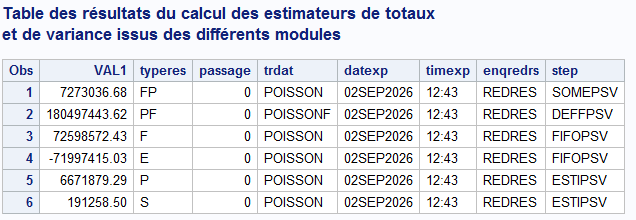
\includegraphics[width=0.9\linewidth]{figures/Poulpe_SRS_NR_CAL_THREE} \end{center}

Both come from the same source. \texttt{Poulpe} does not use the
dissemination weight to expand the sample: it rebuilds the design
weights from the auxiliary table that describes the sampling tree, in
which the population size of each stage is declared as a count. The
rounding makes the reconstructed area weight differ from the one used in
R by a factor of \(1.0042\) here, which propagates to the point
estimate. The same factor explains the variance. Applying it to the
Poulpe total gives \(7242263\), which is the R estimate.

The gap is below half a percent and has no practical consequence. It is
worth knowing only when comparing the two tools digit by digit: the
difference lies in how the population sizes are declared to
\texttt{Poulpe}, not in the variance estimator itself.

\begin{verbatim}
#> Joining with `by = join_by(typeres)`
\end{verbatim}

\begin{table}[t]
\caption{\label{tab:unnamed-chunk-28}Variance elements for Poulpe calculated from gustave} 
\fontsize{12.0pt}{14.0pt}\selectfont
\begin{tabular*}{\linewidth}{@{\extracolsep{\fill}}lllr}
\toprule
Component & typeres & gustave & value \\ 
\midrule\addlinespace[2.5pt]
Point estimate & S & est & 190449.2 \\ 
Sampling variance & P & `var\_srs()` component & 6643647.6 \\ 
F-Non-response component & F &  & 71985478.1 \\ 
E-Non-response component & E &  & -52116123.9 \\ 
Non-response variance & E+F & `var\_pois()` component & 19869354.3 \\ 
? & PF & ? & NA \\ 
Total variance & FP & var & 26513001.9 \\ 
\bottomrule
\end{tabular*}
\end{table}

\section{Practical Implementation}\label{practical-implementation}

\subsection{Overview}\label{overview}

In practice, a variance estimation wrapper must be created for each
survey wave that has been extrapolated. One wrapper is needed per level
of analysis (individuals, dwellings), since each level involves
different stages of the sampling design.

When the sampling design is simple --- a (possibly stratified) simple
random sample --- the \texttt{qvar()} function is fully sufficient to
create the wrapper. It natively handles stratification, non-response
correction and calibration, and its only limitation is that it supports
only a single sampling stage.

For multistage designs --- the common case for household surveys ---
\texttt{qvar\_ms()} extends the same declarative interface to an
arbitrary number of stages: stratified simple random sampling at each
stage, non-response correction at any subset of stages, calibration at a
chosen stage, and configurable treatments for single-unit strata. It
also preserves the intermediate information that quality reports and
methodological analysis require: variance components by stage, design
effects, non-response and domain diagnostics are available at estimation
time through the \texttt{diagnostics} parameter, and the wrapper itself
can be audited with \texttt{qvar\_notes()} and
\texttt{inspect\_wrapper()}. For most surveys, \texttt{qvar\_ms()} is
therefore the recommended entry point, and this section details all the
steps required to build a production-ready wrapper with it, from data
preparation through customisation and usage.

Beyond this scope --- unequal inclusion probabilities within strata,
balanced sampling, shared or integrated weights ---
\texttt{define\_variance\_wrapper()} can, in principle, handle any
situation, and it is the foundation on which both \texttt{qvar()} and
\texttt{qvar\_ms()} are built. Writing a wrapper directly with it is,
however, demanding in terms of R programming: the calling conventions of
the variance function have subtle requirements, and the error messages
produced by \texttt{gustave} can be difficult to interpret. It should be
reserved for designs that \texttt{qvar\_ms()} cannot describe.

\subsection{Data Preparation}\label{data-preparation}

Before defining a variance wrapper, the input data must satisfy several
conditions. Failing to check these will produce either cryptic errors
or, worse, silently incorrect variance estimates. \texttt{qvar()} and
\texttt{qvar\_ms()} include a lot of data check to prevent a lot of
errors, while \texttt{define\_variance\_wrapper()} needs your own
quality checks.

\subsubsection{Missing values}\label{missing-values}

Every variable that enters the variance estimation --- inclusion
probabilities, weights, response indicators, calibration variables ---
must be checked for missing values. A common symptom of missing values
is that the wrapper returns nothing for the point estimate
(\texttt{est}). This happens when the \texttt{reference\_weight} vector
contains missing values: since the point estimate is computed as a
weighted sum using \texttt{reference\_weight}, a single \texttt{NA}
propagates to the output.

\begin{Shaded}
\begin{Highlighting}[]
\CommentTok{\# Check for NA in critical variables}
\NormalTok{check\_vars }\OtherTok{\textless{}{-}} \FunctionTok{c}\NormalTok{(}\StringTok{"pik\_area"}\NormalTok{, }\StringTok{"pik\_dwel"}\NormalTok{, }\StringTok{"w\_area"}\NormalTok{, }\StringTok{"w\_dwel"}\NormalTok{, }\StringTok{"prep"}\NormalTok{, }\StringTok{"rep"}\NormalTok{)}
\NormalTok{lfs\_samp\_dwel }\SpecialCharTok{\%\textgreater{}\%}
  \FunctionTok{summarise}\NormalTok{(}\FunctionTok{across}\NormalTok{(}\FunctionTok{all\_of}\NormalTok{(check\_vars), }\SpecialCharTok{\textasciitilde{}} \FunctionTok{sum}\NormalTok{(}\FunctionTok{is.na}\NormalTok{(.x)))) }\SpecialCharTok{\%\textgreater{}\%}
  \FunctionTok{pivot\_longer}\NormalTok{(}\FunctionTok{everything}\NormalTok{(), }\AttributeTok{names\_to =} \StringTok{"variable"}\NormalTok{, }\AttributeTok{values\_to =} \StringTok{"n\_missing"}\NormalTok{) }\SpecialCharTok{\%\textgreater{}\%}
  \FunctionTok{filter}\NormalTok{(n\_missing }\SpecialCharTok{\textgreater{}} \DecValTok{0}\NormalTok{)}

\CommentTok{\# Another possibility, using extrapolation specific function}
\NormalTok{lfs\_samp\_dwel }\SpecialCharTok{\%\textgreater{}\%} 
  \FunctionTok{select}\NormalTok{(}\FunctionTok{all\_of}\NormalTok{(check\_vars)) }\SpecialCharTok{\%\textgreater{}\%} 
  \FunctionTok{plot\_missings}\NormalTok{()}
\end{Highlighting}
\end{Shaded}

For non-response weights specifically when you use
\texttt{define\_variance\_wrapper()}, non-respondents must have a
\texttt{weight\ =\ 0}, not \texttt{NA}. This is because
\texttt{reference\_weight} is set to this weight when defining the
wrapper: non-respondents are given weight zero (meaning they are
excluded from dissemination), but the value must be present.

\begin{Shaded}
\begin{Highlighting}[]
\NormalTok{lfs\_samp\_dwel }\OtherTok{\textless{}{-}}\NormalTok{ lfs\_samp\_dwel }\SpecialCharTok{\%\textgreater{}\%}
  \FunctionTok{mutate}\NormalTok{(}\AttributeTok{w\_final\_nrc =} \FunctionTok{ifelse}\NormalTok{(}\FunctionTok{is.na}\NormalTok{(w\_final\_nrc), }\DecValTok{0}\NormalTok{, w\_final\_nrc))}
\end{Highlighting}
\end{Shaded}

\subsubsection{Identifier sorting}\label{identifier-sorting}

\texttt{gustave} requires that unit identifiers be character vectors,
and it issues a warning if they are not sorted. Internally, the variance
function receives \texttt{y} as a named matrix whose row names
correspond to the \texttt{reference\_id} vector. If the identifiers in
the analyst's data are in a different order, \texttt{gustave} re-aligns
them, but if they are not character vectors, the matching can fail
silently.

\begin{Shaded}
\begin{Highlighting}[]
\NormalTok{lfs\_samp\_area }\OtherTok{\textless{}{-}}\NormalTok{ lfs\_samp\_area }\SpecialCharTok{\%\textgreater{}\%}
  \FunctionTok{mutate}\NormalTok{(}\AttributeTok{id\_area =} \FunctionTok{as.character}\NormalTok{(id\_area)) }\SpecialCharTok{\%\textgreater{}\%}
  \FunctionTok{arrange}\NormalTok{(id\_area)}

\NormalTok{lfs\_samp\_dwel }\OtherTok{\textless{}{-}}\NormalTok{ lfs\_samp\_dwel }\SpecialCharTok{\%\textgreater{}\%}
  \FunctionTok{mutate}\NormalTok{(}\AttributeTok{id\_area =} \FunctionTok{as.character}\NormalTok{(id\_area),}
         \AttributeTok{id\_dwel  =} \FunctionTok{as.character}\NormalTok{(id\_dwel)) }\SpecialCharTok{\%\textgreater{}\%}
  \FunctionTok{arrange}\NormalTok{(id\_dwel)}

\NormalTok{lfs\_samp\_ind }\OtherTok{\textless{}{-}}\NormalTok{ lfs\_samp\_ind }\SpecialCharTok{\%\textgreater{}\%}
  \FunctionTok{mutate}\NormalTok{(}\AttributeTok{id\_area =} \FunctionTok{as.character}\NormalTok{(id\_area),}
         \AttributeTok{id\_dwel  =} \FunctionTok{as.character}\NormalTok{(id\_dwel),}
         \AttributeTok{id\_ind  =} \FunctionTok{as.character}\NormalTok{(id\_ind)) }\SpecialCharTok{\%\textgreater{}\%}
  \FunctionTok{arrange}\NormalTok{(id\_ind)}
\end{Highlighting}
\end{Shaded}

The \texttt{arrange()} step is not strictly mandatory but avoids
warnings and makes debugging easier when inspecting the \texttt{y}
matrix inside the variance function.

\subsubsection{Confidentiality of technical
data}\label{confidentiality-of-technical-data}

The technical data embedded in the wrapper contains the full sampling
information: inclusion probabilities, strata, response probabilities,
calibration variables, and unit identifiers. This information is
permanently stored inside the wrapper object. If the wrapper is saved as
an \texttt{.rds} file and shared with analysts, they gain access to all
of this information.

This has implications for data confidentiality. Two strategies can
mitigate the risk. First, the technical data can be limited to the
strict minimum --- only the variables actually needed by the variance
function. Second, if the wrapper must be shared externally, consider
whether the sampling parameters themselves are sensitive. In most cases,
the analyst only needs the wrapper function, not the underlying
technical data, but \texttt{gustave} does not currently offer a
mechanism to encrypt or hide the technical data.

\begin{Shaded}
\begin{Highlighting}[]
\CommentTok{\# Minimal technical data: only what the variance function needs}
\NormalTok{technical\_data }\OtherTok{\textless{}{-}} \FunctionTok{list}\NormalTok{()}
\NormalTok{technical\_data}\SpecialCharTok{$}\NormalTok{lfs\_samp\_area }\OtherTok{\textless{}{-}}\NormalTok{ lfs\_samp\_area }\SpecialCharTok{\%\textgreater{}\%}
  \FunctionTok{select}\NormalTok{(id\_area, pik\_area, w\_area)}
\NormalTok{technical\_data}\SpecialCharTok{$}\NormalTok{lfs\_samp\_dwel }\OtherTok{\textless{}{-}}\NormalTok{ lfs\_samp\_dwel }\SpecialCharTok{\%\textgreater{}\%}
  \FunctionTok{select}\NormalTok{(id\_dwel, id\_area, pik, w\_area, w\_dwel, w\_final, prep, rep)}
\end{Highlighting}
\end{Shaded}

\subsection{Customising the variance
estimation}\label{customising-the-variance-estimation}

\subsubsection{Customising the Wrapper}\label{customising-the-wrapper}

The \texttt{define\_variance\_wrapper()} function accepts three types of
arguments that are embedded differently in the wrapper.

\textbf{\texttt{technical\_data}} is a named list of data frames or
vectors that the variance function needs. Each element becomes an
argument of the variance function with the matching name. This data is
fixed at wrapper creation time and cannot be changed by the analyst. Use
this for everything that is determined by the survey design: sampling
weights, inclusion probabilities, strata, response indicators, and
calibration variables. For example, all the names of the parameters and
the calibration variables can be set in technical\_data. This allows the
variance function to be reused for another case.

\begin{Shaded}
\begin{Highlighting}[]
\NormalTok{var\_sample\_flex }\OtherTok{\textless{}{-}} \ControlFlowTok{function}\NormalTok{(y, lfs\_samp\_dwel, cal\_vars, id\_dwel, stratum, }
\NormalTok{                            wSmp, prep, wCal) \{}
  
\NormalTok{  variance }\OtherTok{\textless{}{-}} \FunctionTok{list}\NormalTok{()}
  
\NormalTok{  resp }\OtherTok{\textless{}{-}}\NormalTok{ lfs\_samp\_dwel }\SpecialCharTok{\%\textgreater{}\%} \FunctionTok{filter}\NormalTok{(rep }\SpecialCharTok{==} \DecValTok{1}\NormalTok{)}
  
  \CommentTok{\# Use the cal\_vars argument instead of extracting variables from lfs\_samp\_dwel}
\NormalTok{  cal\_form }\OtherTok{\textless{}{-}} \FunctionTok{as.formula}\NormalTok{(}\FunctionTok{paste}\NormalTok{(}\StringTok{"\textasciitilde{}"}\NormalTok{,}\FunctionTok{paste}\NormalTok{(cal\_vars,}\AttributeTok{collapse =} \StringTok{"+"}\NormalTok{)))}
\NormalTok{  x\_cal }\OtherTok{\textless{}{-}} \FunctionTok{model.matrix}\NormalTok{(cal\_form, }\AttributeTok{data =}\NormalTok{ resp)}
  
  \CommentTok{\# Step 1: Replace y with calibration residuals (respondents only)}
\NormalTok{  y[resp[[id\_dwel]], ] }\OtherTok{\textless{}{-}} \FunctionTok{res\_cal}\NormalTok{(}
\NormalTok{    y[resp[[id\_dwel]], ,}\AttributeTok{drop =} \ConstantTok{FALSE}\NormalTok{],}
    \AttributeTok{x =}\NormalTok{ x\_cal,}
    \AttributeTok{w =}\NormalTok{ resp[[wCal]]}
\NormalTok{  )}
  
  \CommentTok{\# Step 2: Non{-}response variance (Poisson, respondents only)}
\NormalTok{  variance[[}\StringTok{"nr"}\NormalTok{]] }\OtherTok{\textless{}{-}} \FunctionTok{var\_pois}\NormalTok{(}
\NormalTok{    y[resp[[id\_dwel]], ,}\AttributeTok{drop =} \ConstantTok{FALSE}\NormalTok{],}
    \AttributeTok{pik =}\NormalTok{ resp[[prep]],}
    \AttributeTok{w   =}\NormalTok{ resp[[wSmp]]}
\NormalTok{  )}
  
  \CommentTok{\# Step 3: Reintroduce non{-}respondents with zeros}
\NormalTok{  y }\OtherTok{\textless{}{-}} \FunctionTok{add\_zero}\NormalTok{(y, }\AttributeTok{rownames =}\NormalTok{ lfs\_samp\_dwel[[id\_dwel]])}
  
  \CommentTok{\# Step 4: Sampling variance (SRS, full sample)}
\NormalTok{  variance[[}\StringTok{"srs"}\NormalTok{]] }\OtherTok{\textless{}{-}} \FunctionTok{var\_srs}\NormalTok{(}
\NormalTok{    y }\SpecialCharTok{/}\NormalTok{ lfs\_samp\_dwel[[prep]],}
    \AttributeTok{pik    =} \DecValTok{1} \SpecialCharTok{/}\NormalTok{ lfs\_samp\_dwel[[wSmp]],}
    \AttributeTok{strata =}\NormalTok{ lfs\_samp\_dwel[[stratum]]}
\NormalTok{  )}
  
  \FunctionTok{Reduce}\NormalTok{(}\StringTok{\textasciigrave{}}\AttributeTok{+}\StringTok{\textasciigrave{}}\NormalTok{, variance)}
\NormalTok{\}}

\CommentTok{\# We need to include the same argument as the variance function}

\NormalTok{technical\_data\_flex }\OtherTok{\textless{}{-}} \FunctionTok{list}\NormalTok{()}
\NormalTok{technical\_data\_flex}\SpecialCharTok{$}\NormalTok{lfs\_samp\_dwel   }\OtherTok{\textless{}{-}}\NormalTok{ lfs\_samp\_dwel}
\NormalTok{technical\_data\_flex}\SpecialCharTok{$}\NormalTok{cal\_vars }\OtherTok{\textless{}{-}} \StringTok{"id\_area"}
\NormalTok{technical\_data\_flex}\SpecialCharTok{$}\NormalTok{id\_dwel  }\OtherTok{\textless{}{-}} \StringTok{"id\_dwel"}
\NormalTok{technical\_data\_flex}\SpecialCharTok{$}\NormalTok{wSmp     }\OtherTok{\textless{}{-}} \StringTok{"w\_final"}
\NormalTok{technical\_data\_flex}\SpecialCharTok{$}\NormalTok{prep     }\OtherTok{\textless{}{-}} \StringTok{"prep"}
\NormalTok{technical\_data\_flex}\SpecialCharTok{$}\NormalTok{wCal     }\OtherTok{\textless{}{-}} \StringTok{"w\_final\_nrc"}
\NormalTok{technical\_data\_flex}\SpecialCharTok{$}\NormalTok{stratum  }\OtherTok{\textless{}{-}} \StringTok{"id\_area"}

\NormalTok{precision\_flex }\OtherTok{\textless{}{-}} \FunctionTok{define\_variance\_wrapper}\NormalTok{(}
  \AttributeTok{variance\_function =}\NormalTok{ var\_sample\_flex,}
  \AttributeTok{technical\_data    =}\NormalTok{ technical\_data\_flex,}
  \AttributeTok{reference\_id      =}\NormalTok{ technical\_data\_flex}\SpecialCharTok{$}\NormalTok{lfs\_samp\_dwel}\SpecialCharTok{$}\NormalTok{id\_dwel,}
  \AttributeTok{reference\_weight  =}\NormalTok{ technical\_data\_flex}\SpecialCharTok{$}\NormalTok{lfs\_samp\_dwel}\SpecialCharTok{$}\NormalTok{w\_final\_nrc,}
  \AttributeTok{default\_id        =} \StringTok{"id\_dwel"}
\NormalTok{)}

\FunctionTok{precision\_flex}\NormalTok{(lfs\_samp\_dwel, }\FunctionTok{total}\NormalTok{(income))}
\CommentTok{\#\textgreater{}                call  n      est  variance     std       cv    lower    upper}
\CommentTok{\#\textgreater{} 1 total(y = income) 80 190449.2 197245302 14044.4 7.374359 162922.6 217975.7}
\end{Highlighting}
\end{Shaded}

\textbf{\texttt{technical\_param}} is a named list of parameters that
control methodological choices. Like \texttt{technical\_data}, each
element becomes an argument of the variance function. The key difference
is that \texttt{technical\_param} values can be overridden by the
analyst at call time, making them ideal for switches such as ``with or
without calibration'' or ``alternative non-response model''.

\begin{Shaded}
\begin{Highlighting}[]
\NormalTok{var\_sample\_flex }\OtherTok{\textless{}{-}} \ControlFlowTok{function}\NormalTok{(y, lfs\_samp\_dwel, cal\_vars, id\_dwel, stratum, }
\NormalTok{                            wSmp, prep, wCal, }\AttributeTok{use\_calibration =} \ConstantTok{TRUE}\NormalTok{) \{}
  
\NormalTok{  variance }\OtherTok{\textless{}{-}} \FunctionTok{list}\NormalTok{()}
  
\NormalTok{  resp }\OtherTok{\textless{}{-}}\NormalTok{ lfs\_samp\_dwel }\SpecialCharTok{\%\textgreater{}\%} \FunctionTok{filter}\NormalTok{(rep }\SpecialCharTok{==} \DecValTok{1}\NormalTok{)}
  
  \ControlFlowTok{if}\NormalTok{ (use\_calibration)\{}
    \CommentTok{\# Use the cal\_vars argument instead of extracting variables from lfs\_samp\_dwel}
\NormalTok{    cal\_form }\OtherTok{\textless{}{-}} \FunctionTok{as.formula}\NormalTok{(}\FunctionTok{paste}\NormalTok{(}\StringTok{"\textasciitilde{}"}\NormalTok{,}\FunctionTok{paste}\NormalTok{(cal\_vars,}\AttributeTok{collapse =} \StringTok{"+"}\NormalTok{)))}
\NormalTok{    x\_cal }\OtherTok{\textless{}{-}} \FunctionTok{model.matrix}\NormalTok{(cal\_form, }\AttributeTok{data =}\NormalTok{ resp)}
    
    \CommentTok{\# Step 1: Replace y with calibration residuals (respondents only)}
\NormalTok{    y[resp[[id\_dwel]], ] }\OtherTok{\textless{}{-}} \FunctionTok{res\_cal}\NormalTok{(}
\NormalTok{      y[resp[[id\_dwel]], ,}\AttributeTok{drop =} \ConstantTok{FALSE}\NormalTok{],}
      \AttributeTok{x =}\NormalTok{ x\_cal,}
      \AttributeTok{w =}\NormalTok{ resp[[wCal]]}
\NormalTok{    )}
\NormalTok{  \}}
  
  \CommentTok{\# Step 2: Non{-}response variance (Poisson, respondents only)}
\NormalTok{  variance[[}\StringTok{"nr"}\NormalTok{]] }\OtherTok{\textless{}{-}} \FunctionTok{var\_pois}\NormalTok{(}
\NormalTok{    y[resp[[id\_dwel]], ,}\AttributeTok{drop =} \ConstantTok{FALSE}\NormalTok{],}
    \AttributeTok{pik =}\NormalTok{ resp[[prep]],}
    \AttributeTok{w   =}\NormalTok{ resp[[wSmp]]}
\NormalTok{  )}
  
  \CommentTok{\# Step 3: Reintroduce non{-}respondents with zeros}
\NormalTok{  y }\OtherTok{\textless{}{-}} \FunctionTok{add\_zero}\NormalTok{(y, }\AttributeTok{rownames =}\NormalTok{ lfs\_samp\_dwel[[id\_dwel]])}
  
  \CommentTok{\# Step 4: Sampling variance (SRS, full sample)}
\NormalTok{  variance[[}\StringTok{"srs"}\NormalTok{]] }\OtherTok{\textless{}{-}} \FunctionTok{var\_srs}\NormalTok{(}
\NormalTok{    y }\SpecialCharTok{/}\NormalTok{ lfs\_samp\_dwel[[prep]],}
    \AttributeTok{pik    =} \DecValTok{1} \SpecialCharTok{/}\NormalTok{ lfs\_samp\_dwel[[wSmp]],}
    \AttributeTok{strata =}\NormalTok{ lfs\_samp\_dwel[[stratum]]}
\NormalTok{  )}
  
  \FunctionTok{Reduce}\NormalTok{(}\StringTok{\textasciigrave{}}\AttributeTok{+}\StringTok{\textasciigrave{}}\NormalTok{, variance)}
\NormalTok{\}}

\NormalTok{technical\_data\_flex }\OtherTok{\textless{}{-}} \FunctionTok{list}\NormalTok{()}
\NormalTok{technical\_data\_flex}\SpecialCharTok{$}\NormalTok{lfs\_samp\_dwel   }\OtherTok{\textless{}{-}}\NormalTok{ lfs\_samp\_dwel}
\NormalTok{technical\_data\_flex}\SpecialCharTok{$}\NormalTok{cal\_vars }\OtherTok{\textless{}{-}} \StringTok{"id\_area"}
\NormalTok{technical\_data\_flex}\SpecialCharTok{$}\NormalTok{id\_dwel  }\OtherTok{\textless{}{-}} \StringTok{"id\_dwel"}
\NormalTok{technical\_data\_flex}\SpecialCharTok{$}\NormalTok{wSmp     }\OtherTok{\textless{}{-}} \StringTok{"w\_final"}
\NormalTok{technical\_data\_flex}\SpecialCharTok{$}\NormalTok{prep     }\OtherTok{\textless{}{-}} \StringTok{"prep"}
\NormalTok{technical\_data\_flex}\SpecialCharTok{$}\NormalTok{wCal     }\OtherTok{\textless{}{-}} \StringTok{"w\_final\_nrc"}
\NormalTok{technical\_data\_flex}\SpecialCharTok{$}\NormalTok{stratum  }\OtherTok{\textless{}{-}} \StringTok{"id\_area"}

\CommentTok{\# We need to create another list for technical parameters.}
\NormalTok{technical\_param\_flex }\OtherTok{\textless{}{-}} \FunctionTok{list}\NormalTok{()}
\NormalTok{technical\_param\_flex}\SpecialCharTok{$}\NormalTok{use\_calibration }\OtherTok{\textless{}{-}} \ConstantTok{TRUE}

\NormalTok{precision\_flex }\OtherTok{\textless{}{-}} \FunctionTok{define\_variance\_wrapper}\NormalTok{(}
  \AttributeTok{variance\_function =}\NormalTok{ var\_sample\_flex,}
  \AttributeTok{technical\_data    =}\NormalTok{ technical\_data\_flex,}
  \AttributeTok{technical\_param   =}\NormalTok{ technical\_param\_flex,}
  \AttributeTok{reference\_id      =}\NormalTok{ technical\_data\_flex}\SpecialCharTok{$}\NormalTok{lfs\_samp\_dwel}\SpecialCharTok{$}\NormalTok{id\_dwel,}
  \AttributeTok{reference\_weight  =}\NormalTok{ technical\_data\_flex}\SpecialCharTok{$}\NormalTok{lfs\_samp\_dwel}\SpecialCharTok{$}\NormalTok{w\_final\_nrc,}
  \AttributeTok{default\_id        =} \StringTok{"id\_dwel"}
\NormalTok{)}

\CommentTok{\# Analyst can override:}
\FunctionTok{precision\_flex}\NormalTok{(lfs\_samp\_dwel, }\FunctionTok{total}\NormalTok{(income)) }\CommentTok{\# with calibration (default)}
\CommentTok{\#\textgreater{}                call  n      est  variance     std       cv    lower    upper}
\CommentTok{\#\textgreater{} 1 total(y = income) 80 190449.2 197245302 14044.4 7.374359 162922.6 217975.7}
\FunctionTok{precision\_flex}\NormalTok{(lfs\_samp\_dwel, }\FunctionTok{total}\NormalTok{(income), }\AttributeTok{use\_calibration =} \ConstantTok{FALSE}\NormalTok{) }\CommentTok{\# without calibration}
\CommentTok{\#\textgreater{}                call  n      est  variance      std       cv    lower  upper}
\CommentTok{\#\textgreater{} 1 total(y = income) 80 190449.2 524074026 22892.66 12.02035 145580.4 235318}
\end{Highlighting}
\end{Shaded}

\textbf{\texttt{objects\_to\_include}} is a character vector naming R
objects in the current environment that should be included in the
wrapper. This is for advanced use cases --- for instance, including a
custom helper function that the variance function calls internally. In
most situations, \texttt{technical\_data} and \texttt{technical\_param}
are sufficient.

\subsubsection{Customising the variance
function}\label{customising-the-variance-function}

The variance function is where the methodological work happens. Its
interface must follow a strict pattern: it receives exactly one unnamed
``data'' argument (\texttt{y}, the matrix of variables of interest) and
any number of named arguments matching the elements of
\texttt{technical\_data} and \texttt{technical\_param}.

\textbf{Input}. y is a numeric matrix with one column per variable of
interest and row names corresponding to the unit identifiers (matching
\texttt{reference\_id}). When the analyst calls
\texttt{precision(data,\ total(income))}, the total statistic wrapper
extracts the income column, and passes the result as \texttt{y}. This
means that \texttt{y} does not already contain the weighted values.

\textbf{Output}. By default, the function must return the estimated
variance for the corresponding variable of interest. If the function
returns anything else, \texttt{gustave} will raise an error. A
customisation of the statistic wrappers allows more options.

\textbf{Diagnostic output}. Within the variance function,
\texttt{print()} can be used to display intermediate results. These
messages appear in the console when the wrapper is called and can be
useful for debugging. However, they cannot be captured programmatically
by the analyst.

For production use, a better approach is to store diagnostic information
in a separate environment that persists across calls:

\begin{Shaded}
\begin{Highlighting}[]
\CommentTok{\# Create a persistent environment for diagnostics}
\NormalTok{diag\_env }\OtherTok{\textless{}{-}} \FunctionTok{new.env}\NormalTok{(}\AttributeTok{parent =} \FunctionTok{emptyenv}\NormalTok{())}

\NormalTok{var\_sample\_diag }\OtherTok{\textless{}{-}} \ControlFlowTok{function}\NormalTok{(y, lfs\_samp\_area, lfs\_samp\_dwel, lfs\_samp\_ind) \{}
\NormalTok{  variance }\OtherTok{\textless{}{-}} \FunctionTok{list}\NormalTok{()}
  
  \CommentTok{\# ... compute variance components ...}
  
\NormalTok{  poulpe\_F          }\OtherTok{\textless{}{-}} \DecValTok{0}
\NormalTok{  variance[[}\StringTok{"nr"}\NormalTok{]]  }\OtherTok{\textless{}{-}} \DecValTok{1000}
\NormalTok{  variance[[}\StringTok{"srs"}\NormalTok{]] }\OtherTok{\textless{}{-}} \DecValTok{1000}

  \CommentTok{\# Store diagnostics}
\NormalTok{  diag\_env}\SpecialCharTok{$}\NormalTok{components }\OtherTok{\textless{}{-}}\NormalTok{ variance}
\NormalTok{  diag\_env}\SpecialCharTok{$}\NormalTok{poulpe }\OtherTok{\textless{}{-}} \FunctionTok{tibble}\NormalTok{(}
    \AttributeTok{typeres =} \FunctionTok{c}\NormalTok{(}\StringTok{"FP"}\NormalTok{, }\StringTok{"F"}\NormalTok{, }\StringTok{"E"}\NormalTok{, }\StringTok{"P"}\NormalTok{),}
    \AttributeTok{value   =} \FunctionTok{c}\NormalTok{(}\FunctionTok{Reduce}\NormalTok{(}\StringTok{\textasciigrave{}}\AttributeTok{+}\StringTok{\textasciigrave{}}\NormalTok{, variance),}
\NormalTok{                poulpe\_F,}
\NormalTok{                variance[[}\StringTok{"nr"}\NormalTok{]] }\SpecialCharTok{{-}}\NormalTok{ poulpe\_F,}
\NormalTok{                variance[[}\StringTok{"srs"}\NormalTok{]])}
\NormalTok{  )}
  
  \FunctionTok{Reduce}\NormalTok{(}\StringTok{\textasciigrave{}}\AttributeTok{+}\StringTok{\textasciigrave{}}\NormalTok{, variance)}
\NormalTok{\}}

\NormalTok{technical\_data }\OtherTok{\textless{}{-}} \FunctionTok{list}\NormalTok{()}
\NormalTok{technical\_data}\SpecialCharTok{$}\NormalTok{lfs\_samp\_area }\OtherTok{\textless{}{-}}\NormalTok{ lfs\_samp\_area}
\NormalTok{technical\_data}\SpecialCharTok{$}\NormalTok{lfs\_samp\_dwel }\OtherTok{\textless{}{-}}\NormalTok{ lfs\_samp\_dwel}
\NormalTok{technical\_data}\SpecialCharTok{$}\NormalTok{lfs\_samp\_ind  }\OtherTok{\textless{}{-}}\NormalTok{ lfs\_samp\_ind}

\NormalTok{precision }\OtherTok{\textless{}{-}} \FunctionTok{define\_variance\_wrapper}\NormalTok{(}
  \AttributeTok{variance\_function  =}\NormalTok{ var\_sample\_diag,}
  \AttributeTok{technical\_data     =}\NormalTok{ technical\_data,}
  \AttributeTok{objects\_to\_include =} \StringTok{"diag\_env"}\NormalTok{,}
  \AttributeTok{reference\_id       =}\NormalTok{ technical\_data}\SpecialCharTok{$}\NormalTok{lfs\_samp\_ind}\SpecialCharTok{$}\NormalTok{id\_ind,}
  \AttributeTok{reference\_weight   =}\NormalTok{ technical\_data}\SpecialCharTok{$}\NormalTok{lfs\_samp\_ind}\SpecialCharTok{$}\NormalTok{w\_final\_nrc,}
  \AttributeTok{default\_id         =} \StringTok{"id\_ind"}
\NormalTok{)}

\CommentTok{\# After calling the wrapper, diagnostics are available:}
\FunctionTok{precision}\NormalTok{(lfs\_samp\_ind, }\FunctionTok{total}\NormalTok{(income))}
\CommentTok{\#\textgreater{}                call   n      est variance      std         cv    lower    upper}
\CommentTok{\#\textgreater{} 1 total(y = income) 116 190449.2     2000 44.72136 0.02348205 190361.5 190536.8}
\NormalTok{diag\_env}\SpecialCharTok{$}\NormalTok{components}
\CommentTok{\#\textgreater{} $nr}
\CommentTok{\#\textgreater{} [1] 1000}
\CommentTok{\#\textgreater{} }
\CommentTok{\#\textgreater{} $srs}
\CommentTok{\#\textgreater{} [1] 1000}
\NormalTok{diag\_env}\SpecialCharTok{$}\NormalTok{poulpe}
\CommentTok{\#\textgreater{} \# A tibble: 4 x 2}
\CommentTok{\#\textgreater{}   typeres value}
\CommentTok{\#\textgreater{}   \textless{}chr\textgreater{}   \textless{}dbl\textgreater{}}
\CommentTok{\#\textgreater{} 1 FP       2000}
\CommentTok{\#\textgreater{} 2 F           0}
\CommentTok{\#\textgreater{} 3 E        1000}
\CommentTok{\#\textgreater{} 4 P        1000}
\end{Highlighting}
\end{Shaded}

Note that this approach has a limitation: since \texttt{gustave} may
call the variance function multiple times (e.g.~for domain estimation
with \texttt{by}), \texttt{diag\_env} will contain only the results from
the last call. For domain estimation, consider accumulating results
rather than overwriting.

\texttt{qvar\_ms()} includes a technical parameter called
\texttt{diagnostics}. With it, you can obtain Variance components
(\texttt{"components"}), Design effect (\texttt{"deff"}), Degrees of
freedom (\texttt{"dof"}), Non-response diagnostics (\texttt{"nr"}) or
Domain sample sizes (\texttt{"domains"}). See the \texttt{qvar\_ms()}
dedicated vignette for diagnostic explanation.

\subsubsection{Customising the statistic
wrappers}\label{customising-the-statistic-wrappers}

\texttt{gustave} ships with standard statistic wrappers:
\texttt{total()}, \texttt{mean()}, \texttt{ratio()}, and
\texttt{diff\_of\_means()}. These handle the linearisation step
automatically. For instance, \texttt{mean()} computes the ratio
estimator and its linearised variable, then passes the linearised
variable to the variance function.

Additional statistic wrappers can be defined using
\texttt{define\_statistic\_wrapper()}. This is useful when the survey
requires a non-standard estimator (e.g., a Gini coefficient, a quantile,
or a rate with a specific denominator).

\begin{Shaded}
\begin{Highlighting}[]
\CommentTok{\# Example: a rate estimator (proportion of population in a subgroup)}
\NormalTok{rate }\OtherTok{\textless{}{-}} \FunctionTok{define\_statistic\_wrapper}\NormalTok{(}
  \AttributeTok{statistic\_function =} \ControlFlowTok{function}\NormalTok{(y, weight) \{}
\NormalTok{    point }\OtherTok{\textless{}{-}} \FunctionTok{sum}\NormalTok{(y }\SpecialCharTok{*}\NormalTok{ weight) }\SpecialCharTok{/} \FunctionTok{sum}\NormalTok{(weight)}
\NormalTok{    lin   }\OtherTok{\textless{}{-}}\NormalTok{ (y }\SpecialCharTok{{-}}\NormalTok{ point) }\SpecialCharTok{/} \FunctionTok{sum}\NormalTok{(weight)}
    \FunctionTok{list}\NormalTok{(}\AttributeTok{point =}\NormalTok{ point, }\AttributeTok{lin =}\NormalTok{ lin)}
\NormalTok{  \},}
  \AttributeTok{arg\_type =} \FunctionTok{list}\NormalTok{(}\AttributeTok{data =} \StringTok{"y"}\NormalTok{, }\AttributeTok{weight =} \StringTok{"weight"}\NormalTok{)}
\NormalTok{)}
\end{Highlighting}
\end{Shaded}

The \texttt{statistic\_function} must return a list with two elements:
\texttt{point} (the point estimate) and \texttt{lin} (the linearised
variable). An optional metadata element can carry additional information
(e.g.~sample size) to the display function.

Custom statistic wrappers are made available inside the variance wrapper
through the \texttt{objects\_to\_include} argument:

\begin{Shaded}
\begin{Highlighting}[]
\NormalTok{precision }\OtherTok{\textless{}{-}} \FunctionTok{define\_variance\_wrapper}\NormalTok{(}
  \AttributeTok{variance\_function  =}\NormalTok{ var\_sample,}
  \AttributeTok{technical\_data     =}\NormalTok{ technical\_data,}
  \AttributeTok{objects\_to\_include =} \StringTok{"rate"}\NormalTok{,}
  \AttributeTok{reference\_id       =}\NormalTok{ technical\_data}\SpecialCharTok{$}\NormalTok{lfs\_samp\_ind}\SpecialCharTok{$}\NormalTok{id\_ind,}
  \AttributeTok{reference\_weight   =}\NormalTok{ technical\_data}\SpecialCharTok{$}\NormalTok{lfs\_samp\_ind}\SpecialCharTok{$}\NormalTok{w\_final\_nrc,}
  \AttributeTok{default\_id         =} \StringTok{"id\_ind"}
\NormalTok{)}

\CommentTok{\# Now the analyst can use:}
\FunctionTok{precision}\NormalTok{(data\_mb, }\FunctionTok{rate}\NormalTok{(unemployed))}
\end{Highlighting}
\end{Shaded}

\subsubsection{Customising the display
function}\label{customising-the-display-function}

By default, \texttt{gustave} displays results using
\texttt{standard\_display()}, which shows the estimate, variance,
standard error, coefficient of variation, and confidence interval
bounds. This default can be replaced when defining a custom statistic
wrapper, by passing a \texttt{display\_function} argument.

A custom display function receives the point estimate, the variance, and
any metadata returned by the statistic function. It should return a
named vector or a one-row data frame. You can add information that comes
from the full estimation pipeline: variance components,
\texttt{Poulpe}-equivalent decompositions, sample sizes, or warning
flags.

\subsection{\texorpdfstring{Multistage variance estimation with
\texttt{qvar\_ms()}}{Multistage variance estimation with qvar\_ms()}}\label{multistage-variance-estimation-with-qvar_ms}

The \texttt{qvar()} function performs analytical variance estimation in
the most common single-stage case: stratified simple random sampling,
non-response correction through reweighting, calibration on margins.
\texttt{qvar\_ms()} extends this logic to \textbf{multistage designs}:
units of stage 2 are drawn within the units of stage 1, units of stage 3
within the units of stage 2, and so on, with non-response correction
possibly occurring at each stage and calibration at one given stage.

The variance is estimated as the sum of the conditional variances of
each stage, following the Rao (1975) formula as implemented in the SAS
Poulpe macros (Caron, 1998) and natively supported by the variance
functions of the gustave package: at each stage, the variance
contributions (\texttt{var\_srs()}, \texttt{var\_pois()}) are
\emph{linearly} weighted by the cumulated corrected weight of the stages
above, through their \texttt{w} argument, and the first-stage variance
is computed on the estimated totals per primary sampling unit.

A dedicated vignette \emph{Multistage variance estimation with qvar\_ms}
walks through \textbf{nine cases of increasing complexity}, using the
same datasets, to explain how to use \texttt{qvar\_ms()}.

With \texttt{qvar\_ms()}, a lot a sampling designs is now covered with a
lot of integrity data check and methodological notes. For the most
complex or unusual designs (atypical sampling schemes, non-standard
non-response models, or experimental weighting procedures) there is
little value in building a generic function. In those cases, it is more
efficient to work directly with \texttt{define\_variance\_wrapper()} and
a custom variance function tailored to the specific situation.

\subsection{Inspecting a variance
wrapper}\label{inspecting-a-variance-wrapper}

Once a variance wrapper has been defined through \texttt{qvar()},
\texttt{qvar\_ms()} or \texttt{define\_variance\_wrapper()}, it can be
useful to verify its internal structure before use it in production. The
\texttt{inspect\_wrapper()} function performs this diagnostic by
extracting the reference population, the technical data inventory, and
the variance estimation pipeline directly from the wrapper object.

This is particularly valuable for documentation and quality reporting:
it provides a visual confirmation that the wrapper implements the
intended sampling design, with the correct sequence of calibration,
non-response correction, aggregation, and variance computation steps. To
attach to a quality report or to share with a colleague,
\texttt{inspect\_wrapper()} can generate a self-contained HTML file.
Here is an example for the variance function with SRS, non-response and
calibration at dwelling level.

\texttt{inspect\_wrapper()} can also inspect a \texttt{qvar\_ms()}
object. Because of the structure of the \texttt{qvar\_ms()} object (in
list for each stage of sampling), \texttt{inspect\_wrapper()} call an
intern function \texttt{inspect\_wrapper\_ms()} with more information
about the wrapper.

\begin{Shaded}
\begin{Highlighting}[]
\FunctionTok{inspect\_wrapper}\NormalTok{(precision\_cal, }\AttributeTok{file =} \StringTok{"inspect\_precision\_cal.html"}\NormalTok{)}
\end{Highlighting}
\end{Shaded}

\begin{center}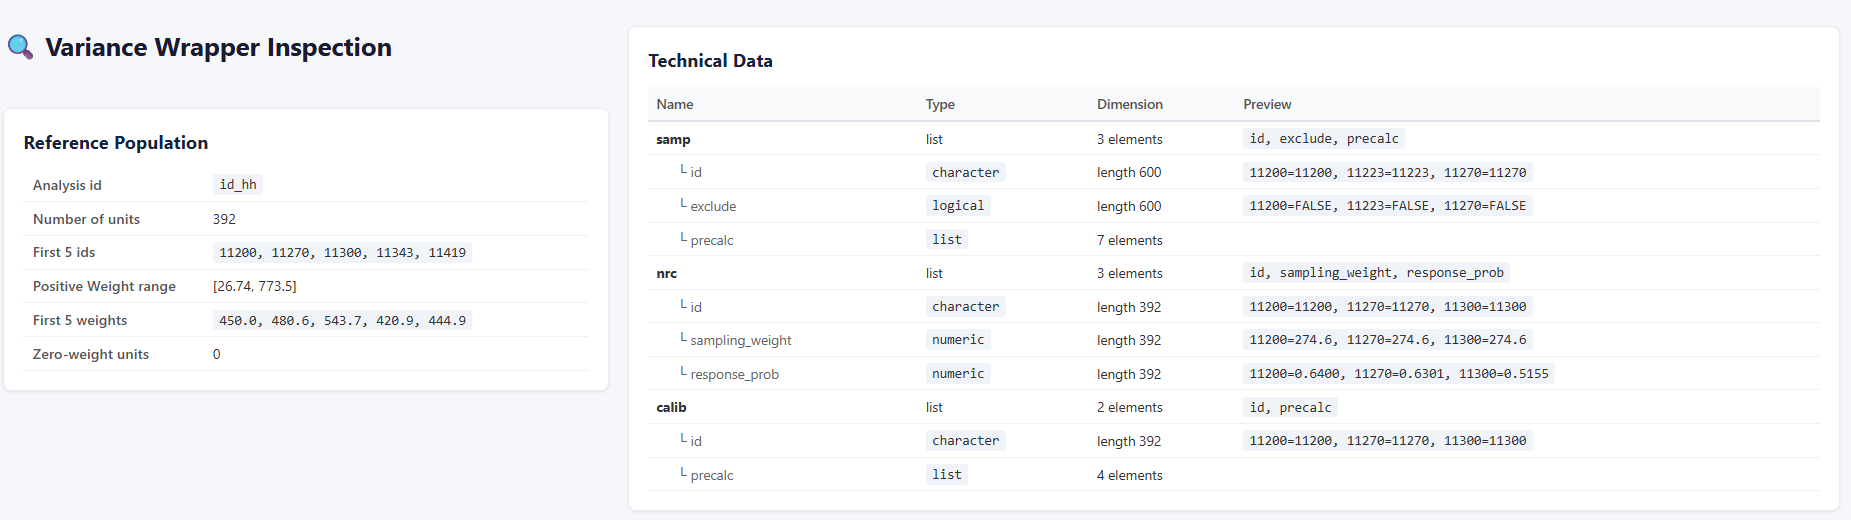
\includegraphics[width=1\linewidth]{figures/inspect_infos} \end{center}

\begin{center}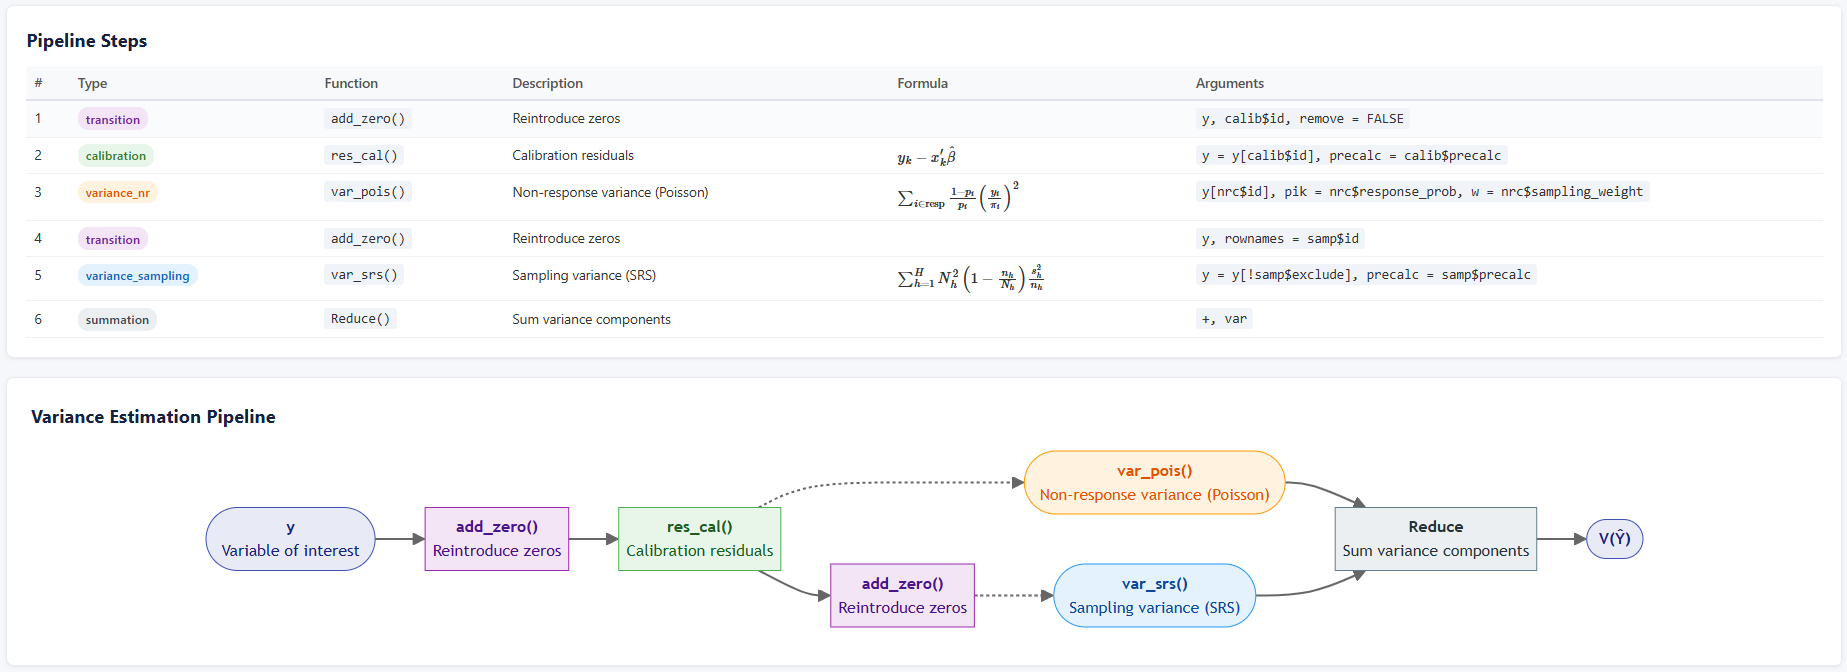
\includegraphics[width=1\linewidth]{figures/inspect_pipeline1} \end{center}

\subsection{Using the Variance
Wrapper}\label{using-the-variance-wrapper}

Everything in this section applies equally to wrappers created with
\texttt{qvar()}, \texttt{qvar\_ms()} and with
\texttt{define\_variance\_wrapper()}. Once defined, a wrapper is simply
a function that takes a data frame and one or more statistic
expressions.

\subsubsection{Basic usage}\label{basic-usage}

\begin{Shaded}
\begin{Highlighting}[]
\CommentTok{\# Single statistic}
\FunctionTok{precision\_cal}\NormalTok{(data\_hh, }\FunctionTok{total}\NormalTok{(income))}

\CommentTok{\# Multiple statistics with labels}
\FunctionTok{precision\_cal}\NormalTok{(data\_hh,}
  \StringTok{"Total income"}      \OtherTok{=} \FunctionTok{total}\NormalTok{(income),}
  \StringTok{"Mean income"}       \OtherTok{=} \FunctionTok{mean}\NormalTok{(income),}
  \StringTok{"Unemployment rate"} \OtherTok{=} \FunctionTok{ratio}\NormalTok{(unemployed, active)}
\NormalTok{)}
\end{Highlighting}
\end{Shaded}

\subsubsection{\texorpdfstring{Domain estimation with \texttt{where} and
\texttt{by}}{Domain estimation with where and by}}\label{domain-estimation-with-where-and-by}

The \texttt{where} argument restricts estimation to a subpopulation
(domain). The \texttt{by} argument repeats the estimation for each level
of a grouping variable. Both can be combined.

\begin{Shaded}
\begin{Highlighting}[]
\CommentTok{\# Domain estimation}
\FunctionTok{precision\_cal}\NormalTok{(data\_hh, }\FunctionTok{mean}\NormalTok{(income), }\AttributeTok{where =}\NormalTok{ region }\SpecialCharTok{==} \StringTok{"Flanders"}\NormalTok{)}

\CommentTok{\# Estimation by group}
\FunctionTok{precision\_cal}\NormalTok{(data\_hh, }\FunctionTok{mean}\NormalTok{(income), }\AttributeTok{by =}\NormalTok{ region)}

\CommentTok{\# Combined}
\FunctionTok{precision\_cal}\NormalTok{(data\_hh, }\FunctionTok{mean}\NormalTok{(income), }\AttributeTok{by =}\NormalTok{ sex, }\AttributeTok{where =}\NormalTok{ age\_cat }\SpecialCharTok{==} \StringTok{"25{-}49"}\NormalTok{)}
\end{Highlighting}
\end{Shaded}

\subsubsection{Integration with tidyverse
workflows}\label{integration-with-tidyverse-workflows}

The output of a variance wrapper is a data frame, which makes it
straightforward to integrate into tidyverse pipelines. However, because
\texttt{gustave} wrappers rely on non-standard evaluation (the statistic
expression is passed unquoted, e.g.~\texttt{total(income)} rather than
\texttt{"total(income)"}), calling them programmatically --- in a loop
over multiple variables or breakdowns --- requires some care.

A practical approach is to build the wrapper call as a string and
evaluate it with \texttt{eval(parse(text\ =\ ...))}. While this is not
idiomatic tidyverse style, it is the most reliable way to interact with
\texttt{gustave}'s non-standard evaluation from within a loop. Two
helper functions make this manageable.

\texttt{call\_gustave()} handles a single call to the wrapper for one
indicator and an optional set of grouping variables. When multiple
grouping variables are specified (e.g.~estimating by region and sex
simultaneously), it creates a temporary interaction variable, passes it
to the \texttt{by} argument, and splits the result back into separate
columns afterwards.

\begin{Shaded}
\begin{Highlighting}[]
\FunctionTok{call\_gustave}\NormalTok{(lfs\_samp\_dwel,}\StringTok{"income"}\NormalTok{,}\AttributeTok{wrapper =} \StringTok{"precision\_cal"}\NormalTok{,}\AttributeTok{fun\_name =} \StringTok{"total"}\NormalTok{)}
\CommentTok{\#\textgreater{} Warning: 32 observations do not match any responding units of the survey. They are discarded.}
\CommentTok{\#\textgreater{}                call  n      est  variance     std       cv    lower    upper}
\CommentTok{\#\textgreater{} 1 total(y = income) 48 190449.2 197245302 14044.4 7.374359 162922.6 217975.7}
\CommentTok{\#\textgreater{}    indic}
\CommentTok{\#\textgreater{} 1 income}
\end{Highlighting}
\end{Shaded}

\texttt{batch\_gustave()} orchestrates the full estimation process.
Given a wrapper, a statistic function name, a list of indicator
variables, and optional grouping and domain variables, it runs four
successive steps: overall estimates with no breakdown, marginal
estimates for each grouping or domain variable separately, crossed
estimates combining all grouping variables, and crossed group estimates
within each domain. The output is a single tidy data frame with a
human-readable pop column describing the subpopulation (e.g.~``region =
Flanders ; sex = M''), ready for export to quality reports.

\begin{Shaded}
\begin{Highlighting}[]
\CommentTok{\# Example: estimate total and mean for two variables,}
\CommentTok{\# by region and sex (crossed), with id\_area as a domain}
\FunctionTok{set.seed}\NormalTok{(}\DecValTok{123}\NormalTok{)}
\NormalTok{lfs\_samp\_ind}\SpecialCharTok{$}\NormalTok{sex }\OtherTok{\textless{}{-}} \FunctionTok{sample}\NormalTok{(}\FunctionTok{c}\NormalTok{(}\StringTok{"M"}\NormalTok{,}\StringTok{"F"}\NormalTok{),}\FunctionTok{nrow}\NormalTok{(lfs\_samp\_ind), }\AttributeTok{replace=}\NormalTok{T)}

\NormalTok{results }\OtherTok{\textless{}{-}} \FunctionTok{batch\_gustave}\NormalTok{(}
  \AttributeTok{df          =}\NormalTok{ lfs\_samp\_ind,}
  \AttributeTok{wrapper     =} \StringTok{"precision\_three\_2"}\NormalTok{,}
  \AttributeTok{fun\_name    =} \StringTok{"mean"}\NormalTok{,}
  \AttributeTok{vars\_indics =} \FunctionTok{c}\NormalTok{(}\StringTok{"income"}\NormalTok{,}\StringTok{"unemp"}\NormalTok{),}
  \AttributeTok{vars\_groups =} \StringTok{"sex"}\NormalTok{,}
  \AttributeTok{vars\_domain =} \StringTok{"id\_area"}
\NormalTok{)}

\CommentTok{\# The result is a tidy data frame:}
\NormalTok{results }\SpecialCharTok{\%\textgreater{}\%} 
  \FunctionTok{group\_by}\NormalTok{(indic) }\SpecialCharTok{\%\textgreater{}\%} 
  \FunctionTok{slice\_min}\NormalTok{(cv,}\AttributeTok{n =} \DecValTok{5}\NormalTok{) }\SpecialCharTok{\%\textgreater{}\%} 
  \FunctionTok{select}\NormalTok{(pop, indic, est, cv, lower, upper)}
\CommentTok{\#\textgreater{} \# A tibble: 10 x 6}
\CommentTok{\#\textgreater{} \# Groups:   indic [2]}
\CommentTok{\#\textgreater{}    pop                      indic      est    cv   lower  upper}
\CommentTok{\#\textgreater{}    \textless{}chr\textgreater{}                    \textless{}chr\textgreater{}    \textless{}dbl\textgreater{} \textless{}dbl\textgreater{}   \textless{}dbl\textgreater{}  \textless{}dbl\textgreater{}}
\CommentTok{\#\textgreater{}  1 id\_area = A005           income 11.4     46.7   0.951 21.8  }
\CommentTok{\#\textgreater{}  2 sex = M                  income 14.5     72.0  {-}5.98  35.1  }
\CommentTok{\#\textgreater{}  3 sex = M                  income 14.5     72.0  {-}5.98  35.1  }
\CommentTok{\#\textgreater{}  4 id\_area = A016 ; sex = M income 14.8     86.6 {-}10.3   39.8  }
\CommentTok{\#\textgreater{}  5 id\_area = A007           income 13.6     90.2 {-}10.4   37.7  }
\CommentTok{\#\textgreater{}  6 id\_area = A007           unemp   0.143  279.   {-}0.637  0.923}
\CommentTok{\#\textgreater{}  7 id\_area = A005           unemp   0.0455 536.   {-}0.432  0.523}
\CommentTok{\#\textgreater{}  8 sex = F                  unemp   0.0967 620.   {-}1.08   1.27 }
\CommentTok{\#\textgreater{}  9 sex = F                  unemp   0.0967 620.   {-}1.08   1.27 }
\CommentTok{\#\textgreater{} 10 ALL                      unemp   0.103  635.   {-}1.18   1.38}
\end{Highlighting}
\end{Shaded}

The distinction between \texttt{vars\_groups} and \texttt{vars\_domain}
is important. Group variables are crossed: if you specify region and
sex, you get estimates for every region × sex combination. Domain
variables are not crossed with each other: if you specify age\_cat as a
domain, you get estimates for each age category, and for each age
category × region × sex combination, but not for age categories crossed
with other domain variables. This mirrors the typical structure of
quality reports, where a few core breakdowns are fully crossed while
additional dimensions are reported separately.

A word of caution when using \texttt{batch\_gustave()}: since it calls
the wrapper repeatedly --- once per indicator, per breakdown, and per
step --- any \texttt{print()} or \texttt{message()} statement inside the
variance function will be executed at every single call. With a dozen
indicators and several grouping variables, this can produce hundreds of
lines of console output, making it difficult to spot genuine warnings.
It is therefore preferable to remove diagnostic \texttt{print()}
statements from the variance function before running a batch estimation.

The full source code of \texttt{call\_gustave()} and
\texttt{batch\_gustave()} is available in the package
\texttt{extrapolation}.

\section{Conclusion}\label{conclusion}

This vignette has demonstrated how the \texttt{gustave} package can
fully replace the SAS \texttt{Poulpe} macro for analytical variance
estimation in complex dwelling surveys. Starting from stratified simple
random sampling and progressively adding non-response correction,
calibration, and multi-stage sampling, we have shown that
\texttt{gustave} reproduces \texttt{Poulpe} results while offering a
more flexible and transparent framework.

The key advantage of \texttt{gustave} is its wrapper mechanism: once a
variance estimation methodology has been encoded by the methodologist,
analysts can compute precision measures on their own datasets without
needing to understand the underlying formulas. The wrapper is a
self-contained R object that can be saved, shared, and reused across
survey waves.

However, this flexibility comes at a cost. Unlike \texttt{Poulpe}, which
imposes a rigid but predictable structure through its tree-based
configuration, \texttt{gustave} requires the methodologist to have a
thorough understanding of the variance decomposition formulas and their
translation into R code. Errors in the variance function --- wrong
ordering of steps, incorrect inclusion probabilities, mishandled
non-response corrections --- can produce silently incorrect results.

AJOUT PARAGRAPHE SUR QVAR\_MS()

To mitigate this risk, we have presented several strategies. Second,
making variance functions configurable through \texttt{technical\_data}
and \texttt{technical\_param} reduces the need to modify source code
across survey waves. Third, the \texttt{inspect\_wrapper()} diagnostic
tool provides a visual verification of the pipeline before any
estimation is run.

Taken together, these tools support a clear division of labour:
methodologists prepare robust wrappers with the appropriate variance
decomposition, and thematic analysts use them as black-box functions
through \texttt{batch\_gustave()} to produce quality reports. This
collaborative workflow is further strengthened by the fact that
wrappers, as self-contained R functions, can be called from Python
through interfaces such as \texttt{rpy2}, allowing analysts to integrate
variance estimation into their existing pipelines without requiring
expertise in R.

Several topics have not been covered in this vignette. The sampling
designs considered here are all based on simple random sampling (with or
without stratification) at each stage. Designs involving unequal
inclusion probabilities (PPS sampling), balanced sampling (cube method),
or systematic sampling require different variance estimators --- notably
\texttt{varDT()} for the Deville-Tillé approximation or
\texttt{varSYG()} for the Sen-Yates-Grundy estimator --- which
\texttt{gustave} supports but which were outside the scope of this
document.

We have also not compared \texttt{gustave} with the R \texttt{survey}
package, which takes a fundamentally different approach: the analyst
declares the full survey design upfront, and the package handles
variance estimation internally. A systematic comparison --- particularly
regarding the impact of ignoring certain design features --- would be a
valuable complement to this work.

Finally, an important next step is the integration of the variance
estimation output with visualisation tools. Packages such as
\texttt{fonctionr} are specifically designed to produce
publication-quality graphics with properly computed confidence
intervals. Connecting \texttt{gustave} wrappers to such tools would
close the loop between estimation and dissemination, ensuring that the
uncertainty measures produced here are consistently reflected in the
final statistical outputs.

\section{References}\label{references}

\begin{itemize}
\item
  Caron N. (1998), ``Le logiciel Poulpe : aspects méthodologiques'',
  Actes des Journées de méthodologie statistique
  \url{http://jms-insee.fr/jms1998s03_1/} Deville, J.-C. (1993),
  Estimation de la variance pour les enquêtes en deux phases,
  Manuscript, INSEE, Paris.
\item
  Chevalier, Martin, Larbi, Khaled (2018), ``gustave: A User-Oriented
  Statistical Toolkit for Analytical Variance Estimation'', R package
\item
  Deville, J.-C., Tillé, Y. (2005), ``Variance approximation under
  balanced sampling'', Journal of Statistical Planning and Inference,
  128, issue 2 569-591
\item
  Rao, J.N.K (1975), ``Unbiased variance estimation for multistage
  designs'', Sankhya, C n°37
\end{itemize}

\section{Annexe}\label{annexe}

\subsection{Poulpe script to variance
estimation}\label{poulpe-script-to-variance-estimation}

The SAS results used as a benchmark throughout this vignette are
produced with \texttt{\%bouclepoulpe\_total}, an in-house Statbel macro.
\texttt{Poulpe} (Caron, 1998) is the reference SAS system for analytical
variance estimation developed at Insee. Its power comes at the cost of a
verbose interface: a single run requires the sequential invocation of
several steps (reading the sampling design tree, computing inclusion
probabilities, loading the variables of interest, estimating the
variance of totals or of functions of totals), each of which takes
several dozen parameters describing the design, the response phases and
the \texttt{Calmar} calibration. \texttt{\%bouclepoulpe\_total} is
nothing more than a convenience layer built on top of this machinery. It
performs no variance computation of its own: every estimate it returns
is produced by the standard \texttt{Poulpe} steps.

\subsubsection{Case 2: Adding
Non-Response}\label{case-2-adding-non-response-1}

\begin{Shaded}
\begin{Highlighting}[]
\NormalTok{data CALAG.lfs\_samp\_dwel; set R.lfs\_samp\_dwel;}
\NormalTok{NINFFIC = "CA";}
\NormalTok{respons = rep+1;}
\NormalTok{run;}

\NormalTok{DATA BURCE.TREE1;   }
\NormalTok{\%ARBREXXX;}
\NormalTok{infile cards delimiter = "," dsd missover;}
\NormalTok{input nsup ninf typtir ENTAG ENTI ;}
\NormalTok{cards;   }
\NormalTok{ZZ,AA,TOT, ,   }
\NormalTok{AA,BA,EXH,id\_area, id\_area}
\NormalTok{BA,CA,SAS,id\_area,}
\NormalTok{;}
\NormalTok{run;}

\NormalTok{proc sql;}
\NormalTok{create table BURCE.GEO as select distinct}
\NormalTok{    id\_area, (1) AS Auxniv, sum(w\_final) AS NNN}
\NormalTok{from R.lfs\_samp\_dwel group by id\_area;}
\NormalTok{quit;}

\NormalTok{\%let mywip = w\_dwel\_nrc;}
\NormalTok{\%let data\_source = CALAG.lfs\_samp\_dwel;}
\NormalTok{\%let var\_out = T1\_VARIANCE;}
\NormalTok{\%let myArbinp=  TREE1;}
\NormalTok{\%let myDataauxp= GEO;}
\NormalTok{\%let myNbphasp=  2;}
\NormalTok{\%let myPipoissp= PRep;}
\NormalTok{\%let myFormulep= POISSON;}
\NormalTok{\%let myEnqredp = ;}
\NormalTok{\%let myExplicp = ;}
\NormalTok{\%let myExpliqp = ;}

\NormalTok{\%let var1\_TST = 1 = 1;}
\NormalTok{\%let var2\_TST = 1 = 1;}
\NormalTok{\%let var3\_TST = income;}

\NormalTok{\%bouclepoulpe\_total(step1=FP,step2=S);}
\end{Highlighting}
\end{Shaded}

\subsubsection{Case 3: Adding
Calibration}\label{case-3-adding-calibration-1}

\begin{Shaded}
\begin{Highlighting}[]
\NormalTok{data CALAG.lfs\_samp\_dwel; set R.lfs\_samp\_dwel; }
\NormalTok{NINFFIC = "CA";}
\NormalTok{respons = rep+1;}
\NormalTok{run;}

\NormalTok{DATA BURCE.TREE1;   }
\NormalTok{\%ARBREXXX;}
\NormalTok{infile cards delimiter = "," dsd missover;}
\NormalTok{input nsup ninf typtir ENTAG ENTI ;}
\NormalTok{cards;   }
\NormalTok{ZZ,AA,TOT, ,   }
\NormalTok{AA,BA,EXH,id\_area, id\_area}
\NormalTok{BA,CA,SAS,id\_area,}
\NormalTok{;}
\NormalTok{run;}

\NormalTok{proc sql;}
\NormalTok{create table BURCE.GEO as select distinct}
\NormalTok{    id\_area, (1) AS Auxniv, sum(w\_final) AS NNN}
\NormalTok{from R.lfs\_samp\_dwel group by id\_area;}
\NormalTok{quit;}

\NormalTok{\%let mywip = w\_dwel\_nrc;}
\NormalTok{\%let data\_source = CALAG.lfs\_samp\_dwel;}
\NormalTok{\%let var\_out = T2\_VARIANCE;}
\NormalTok{\%let myArbinp=  TREE1;}
\NormalTok{\%let myDataauxp= GEO;}
\NormalTok{\%let myNbphasp=  2;}
\NormalTok{\%let myPipoissp= PRep;}
\NormalTok{\%let myFormulep= POISSON;}
\NormalTok{\%let myEnqredp = REDRES;}
\NormalTok{\%let myExplicp = id\_area;}
\NormalTok{\%let myExpliqp = ;}

\NormalTok{\%let var1\_TST = 1 = 1;}
\NormalTok{\%let var2\_TST = 1 = 1;}
\NormalTok{\%let var3\_TST = income;}

\NormalTok{\%bouclepoulpe\_total(step1=FP,step2=S);}
\end{Highlighting}
\end{Shaded}

\subsubsection{Case 4: Two-Stage
Sampling}\label{case-4-two-stage-sampling-1}

\begin{Shaded}
\begin{Highlighting}[]
\NormalTok{/*********** Paramètres ************/}

\NormalTok{data CALAG.lfs\_samp\_dwel; set R.lfs\_samp\_dwel; }
\NormalTok{strate\_fictive = 1;}
\NormalTok{respons = rep+1;}
\NormalTok{NINFFIC = "DA";}
\NormalTok{run;}

\NormalTok{proc sql; create table CALAG.lfs\_samp\_area as select}
\NormalTok{id\_area,mean(1/pik\_area) as w\_area,}
\NormalTok{1 as strate\_fictive}
\NormalTok{from R.lfs\_samp\_area;}
\NormalTok{quit;}

\NormalTok{DATA BURCE.TREE2;   }
\NormalTok{\%ARBREXXX;}
\NormalTok{infile cards delimiter = "," dsd missover;}
\NormalTok{input nsup ninf typtir ENTAG ENTI ;}
\NormalTok{cards;   }
\NormalTok{ZZ,AA,TOT, ,   }
\NormalTok{AA,BA,EXH,strate\_fictive, strate\_fictive}
\NormalTok{BA,CA,SAS,strate\_fictive, id\_area}
\NormalTok{CA,DA,SAS,strate\_fictive id\_area,}
\NormalTok{;}
\NormalTok{run;}

\NormalTok{proc sql;}
\NormalTok{create table BURCE.GEO2\_A as select distinct}
\NormalTok{    strate\_fictive, (1) AS Auxniv, sum(w\_area) AS NNN}
\NormalTok{from CALAG.lfs\_samp\_area;}

\NormalTok{create table BURCE.GEO2\_B as select distinct}
\NormalTok{    strate\_fictive, id\_area, (2) AS Auxniv, sum(w\_dwel) AS NNN}
\NormalTok{from CALAG.lfs\_samp\_dwel group by id\_area;}
\NormalTok{quit;}

\NormalTok{data BURCE.GEO2; set BURCE.GEO2\_A BURCE.GEO2\_B; run;}

\NormalTok{\%let mywip = w\_dwel\_nrc;}
\NormalTok{\%let data\_source = CALAG.lfs\_samp\_dwel;}
\NormalTok{\%let var\_out = T3\_VARIANCE;}
\NormalTok{\%let myArbinp=  TREE2;}
\NormalTok{\%let myDataauxp= GEO2;}
\NormalTok{\%let myNbphasp=  2;}
\NormalTok{\%let myPipoissp= PRep;}
\NormalTok{\%let myFormulep= POISSON;}
\NormalTok{\%let myEnqredp = REDRES;}
\NormalTok{\%let myExplicp = id\_area;}
\NormalTok{\%let myExpliqp = ;}

\NormalTok{\%let var1\_TST = 1 = 1;}
\NormalTok{\%let var2\_TST = 1 = 1;}
\NormalTok{\%let var3\_TST = income;}

\NormalTok{\%bouclepoulpe\_total(step1=FP,step2=S);}
\end{Highlighting}
\end{Shaded}

\subsubsection{Case 5: Adding individuals
answers}\label{case-5-adding-individuals-answers-1}

\begin{Shaded}
\begin{Highlighting}[]
\NormalTok{/*********** Paramètres ************/}

\NormalTok{/*********** Paramètres ************/}

\NormalTok{data CALAG.lfs\_samp\_ind; set R.lfs\_samp\_ind;}
\NormalTok{strate\_fictive = 1;}
\NormalTok{respons = rep+1;}
\NormalTok{NINFFIC = "EA";}
\NormalTok{run;}

\NormalTok{data CALAG.lfs\_samp\_dwel; set R.lfs\_samp\_dwel;  }
\NormalTok{strate\_fictive = 1;}
\NormalTok{run;}

\NormalTok{proc sql; create table CALAG.lfs\_samp\_area as select}
\NormalTok{id\_area,mean(1/pik\_area) as w\_area,}
\NormalTok{1 as strate\_fictive}
\NormalTok{from R.lfs\_samp\_area;}
\NormalTok{quit;}

\NormalTok{DATA BURCE.TREE3;   }
\NormalTok{\%ARBREXXX;}
\NormalTok{infile cards delimiter = "," dsd missover;}
\NormalTok{input nsup ninf typtir ENTAG ENTI ;}
\NormalTok{cards;   }
\NormalTok{ZZ,AA,TOT, ,   }
\NormalTok{AA,BA,EXH,strate\_fictive, strate\_fictive}
\NormalTok{BA,CA,SAS,strate\_fictive, id\_area}
\NormalTok{CA,DA,SAS,strate\_fictive id\_area, strate\_fictive id\_area id\_dwel}
\NormalTok{DA,EA,EXH,strate\_fictive id\_area id\_dwel, }
\NormalTok{;}
\NormalTok{run;}

\NormalTok{proc sql;}
\NormalTok{create table BURCE.GEO3\_A as select distinct}
\NormalTok{    strate\_fictive, (1) AS Auxniv, round(sum(w\_area)) AS NNN}
\NormalTok{from CALAG.lfs\_samp\_area;}

\NormalTok{create table BURCE.GEO3\_B as select distinct}
\NormalTok{    strate\_fictive, id\_area, (2) AS Auxniv, sum(w\_dwel) AS NNN}
\NormalTok{from CALAG.lfs\_samp\_dwel group by id\_area;}

\NormalTok{create table BURCE.GEO3\_C as select distinct}
\NormalTok{    strate\_fictive, id\_area, id\_dwel, (3) AS Auxniv, sum(w\_ind) AS NNN}
\NormalTok{from CALAG.lfs\_samp\_ind group by id\_dwel;}
\NormalTok{quit;}

\NormalTok{data BURCE.GEO3; set BURCE.GEO3\_A BURCE.GEO3\_B BURCE.GEO3\_C; run;}

\NormalTok{\%let mywip = w\_dwel\_nrc;}
\NormalTok{\%let data\_source = CALAG.lfs\_samp\_ind;}
\NormalTok{\%let var\_out = T4\_VARIANCE;}
\NormalTok{\%let myArbinp=  TREE3;}
\NormalTok{\%let myDataauxp= GEO3;}
\NormalTok{\%let myNbphasp=  2;}
\NormalTok{\%let myPipoissp= PRep;}
\NormalTok{\%let myFormulep= POISSON;}
\NormalTok{\%let myEnqredp = REDRES;}
\NormalTok{\%let myExplicp = id\_area;}
\NormalTok{\%let myExpliqp = ;}

\NormalTok{\%let var1\_TST = 1 = 1;}
\NormalTok{\%let var2\_TST = 1 = 1;}
\NormalTok{\%let var3\_TST = income;}

\NormalTok{\%bouclepoulpe\_total(step1=FP,step2=S);}
\end{Highlighting}
\end{Shaded}


\end{document}
